
\documentclass[a4paper]{article}
\usepackage{subfig}
\usepackage{comment}
\usepackage{caption}
\usepackage{siunitx}%$[\si{\ohm}]$
\usepackage{array}
\usepackage{tabu}
\usepackage{float}
\usepackage{fancyhdr}
\usepackage{amsfonts}
\usepackage{amssymb}
\usepackage{indentfirst}
\usepackage{multirow}
\usepackage{multicol}
\usepackage{enumitem}
\usepackage{float}
\usepackage{amsmath}
\usepackage{listings}
\usepackage{color}
\usepackage{physics}
\usepackage{indentfirst}
\usepackage{enumitem}
\usepackage{mathrsfs}
\usepackage{tikz}
\usepackage[european]{circuitikz}	
\definecolor{codegreen}{rgb}{0,0.6,0}
\definecolor{codegray}{rgb}{0.5,0.5,0.5}
\definecolor{codepurple}{rgb}{0.58,0,0.82}
\definecolor{backcolour}{rgb}{0.95,0.95,0.92}
\lstdefinestyle{mystyle}{
    backgroundcolor=\color{backcolour},   
    commentstyle=\color{codegreen},
    keywordstyle=\color{magenta},
    numberstyle=\tiny\color{codegray},
    stringstyle=\color{codepurple},
    basicstyle=\footnotesize,
    breakatwhitespace=false,         
    breaklines=true,                 
    captionpos=b,                    
    keepspaces=true,                 
    numbers=left,                    
    numbersep=5pt,                  
    showspaces=false,                
    showstringspaces=false,
    showtabs=false,                  
    tabsize=2
}

\lstset{style=mystyle} %Revisar al final
\captionsetup[table]{skip=10pt}

%% Language and font encodings
\usepackage[spanish, es-tabla]{babel}
\usepackage[utf8x]{inputenc}
\usepackage[T1]{fontenc}

%% Sets page size and margins
\usepackage[a4paper,top=3cm,bottom=2cm,left=3cm,right=3cm,marginparwidth=1.75cm]{geometry}

%% Useful packages
\usepackage{amsmath}
\usepackage{graphicx}
%\graphicspath{./images} %Path
\usepackage[colorinlistoftodos]{todonotes}
\usepackage[colorlinks=true, allcolors=blue]{hyperref}

% Informacion portada
\pagestyle{fancy}
\fancyhf{}
\rhead{Procesamiento Digital de Señales y Aplicaciones}
\lhead{ELO313}
\rfoot{\thepage}

%%%%%%%%%%%%%%%%%%%%%% INICIO DOCUMENTO %%%%%%%%%%%%%%%%%%%%%%%%%%%%%%%%%%%%%
\begin{document}
% Portada
\begin{titlepage}
	\centering
	{\scshape\LARGE [ELO313] Procesamiento Digital de Señales y Aplicaciones\par}
	\vspace{1cm}
	%{\scshape\Large Certamen $\#3$\par}
	\vspace{5cm}	
	{\huge\bfseries Certamen $\#3$ \par}
	\vspace{9cm}
	{\Large\Large Mauricio Aravena Cifuentes \\ 201503001-4}
	\vfill
	{\large \ \today \par}
\end{titlepage}
% Informe
\section{Filtrado de señales}
	\subsection{}
		Acerca del filtro se tiene la siguiente información:
		\begin{enumerate}
			\item Es un filtro pasa-alto y tiene un polo en cero
			\item El polo está ubicado a una distancia $r = 0.9$ del origen en el plano-z
			\item Las señales constantes no pasan por el sistema
		\end{enumerate}
		
		A partir de los datos, se puede deducir que se tiene un rechazo para DC, por lo que la ubicación del cero en el plano complejo debe cumplir:
		\begin{equation*}
			z - 1 = 0 \Longleftrightarrow z = 1
		\end{equation*}
		
		Sabiendo que $z = e^{j\omega}$, al evaluar en $\omega = 0$ se tendrá rechazo de la banda DC. Para la ubicación del polo, se sabe conviene que este esté lo más apegado al cero, de esta forma se tendrá un filtro con mayor selectividad, se comportara como un filtro \textit{notch} 	para DC. Por lo que podemos definir la ubicación del polo en $z_{p} = 0.9$. De esta forma la función de transferencia queda de la siguiente forma:
		\begin{equation}
		H(z) = \frac{z-1}{z-0.9}
		\label{eq:1_filter_transfer_function}
		\end{equation}
		
		Realizando el diagrama de polos y ceros:
		\begin{figure}[H]
			\center
			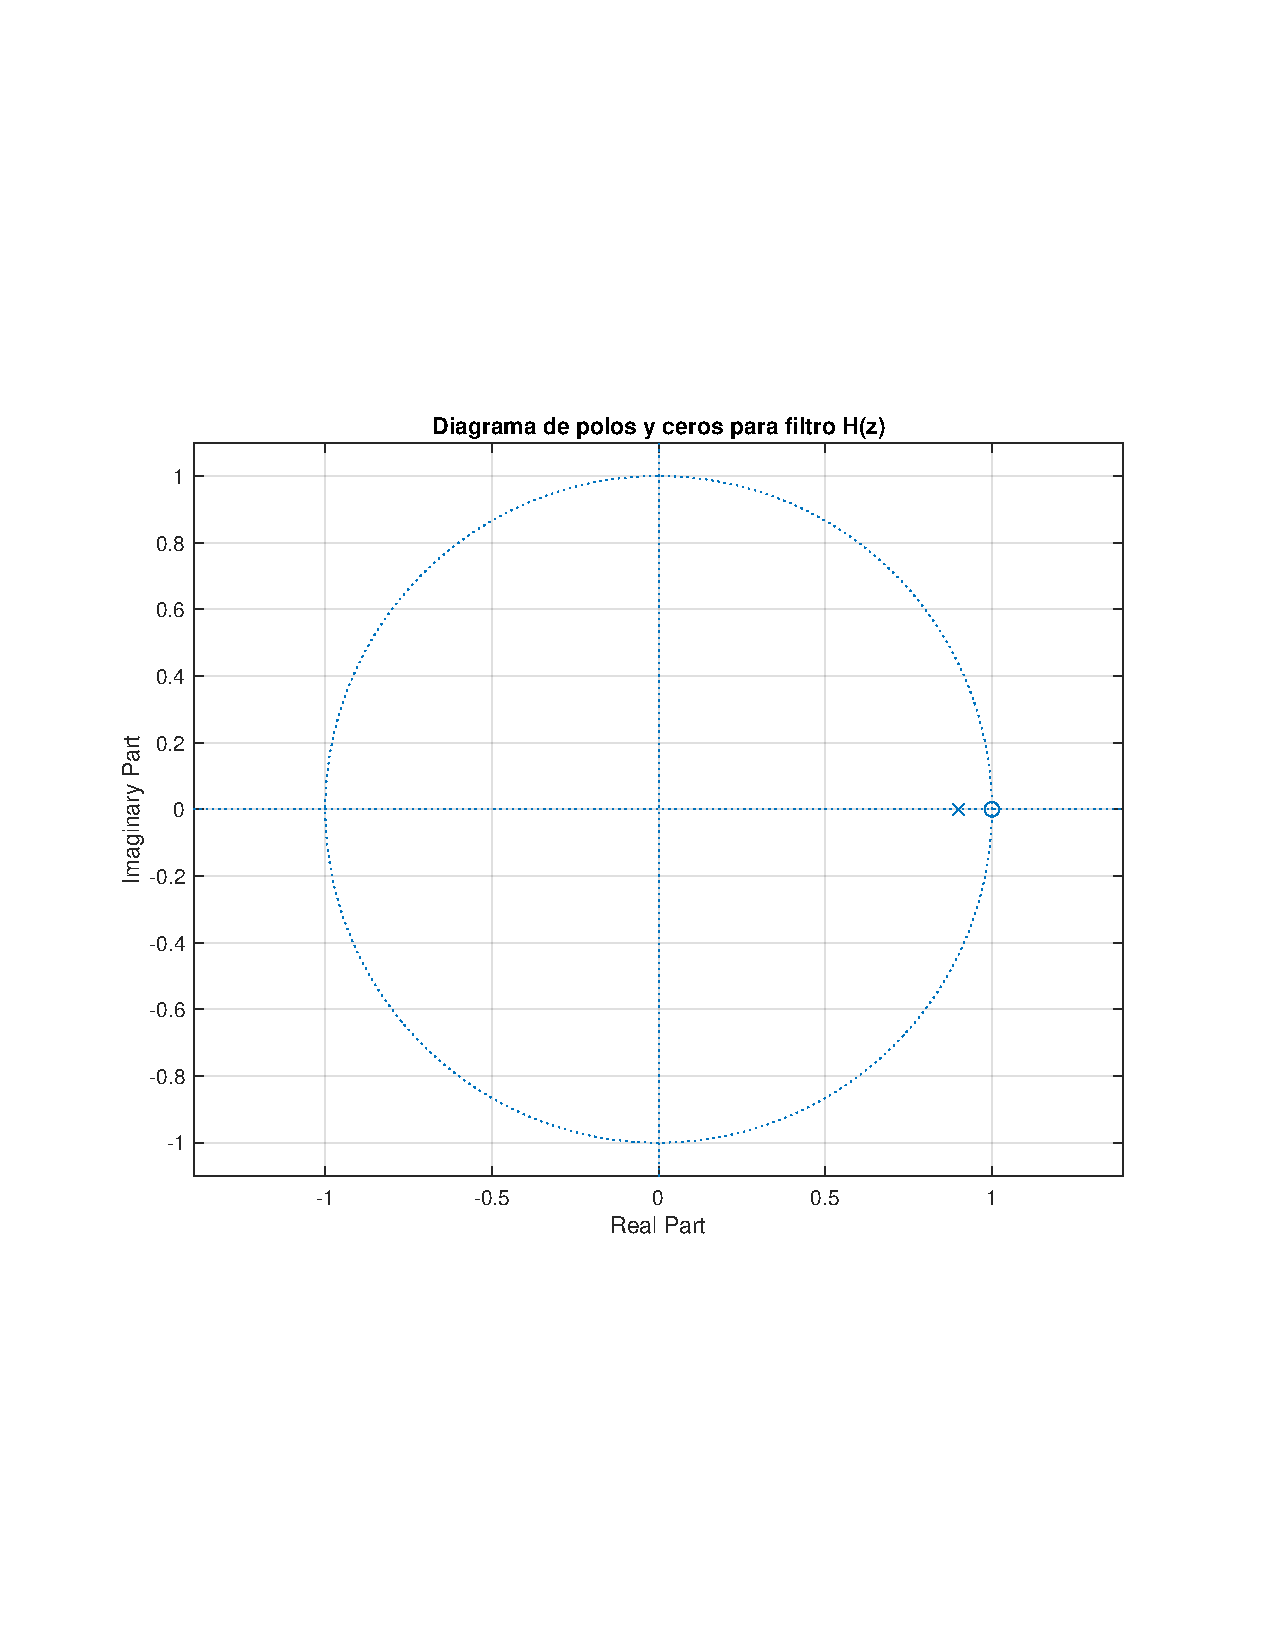
\includegraphics[width=0.6\textwidth,clip, trim = {1.9cm 6.8cm 2.3cm 7cm}]{../plots/1_zp_diag.pdf}
			\caption{Diagrama de polos y ceros para la función de transferencia \ref{eq:1_filter_transfer_function}}
			\label{fig:1_zero_pole_diagram}
		\end{figure}
		
		Analizando la respuesta en magnitud y fase del filtro:
		\begin{figure}[H]
			\center
			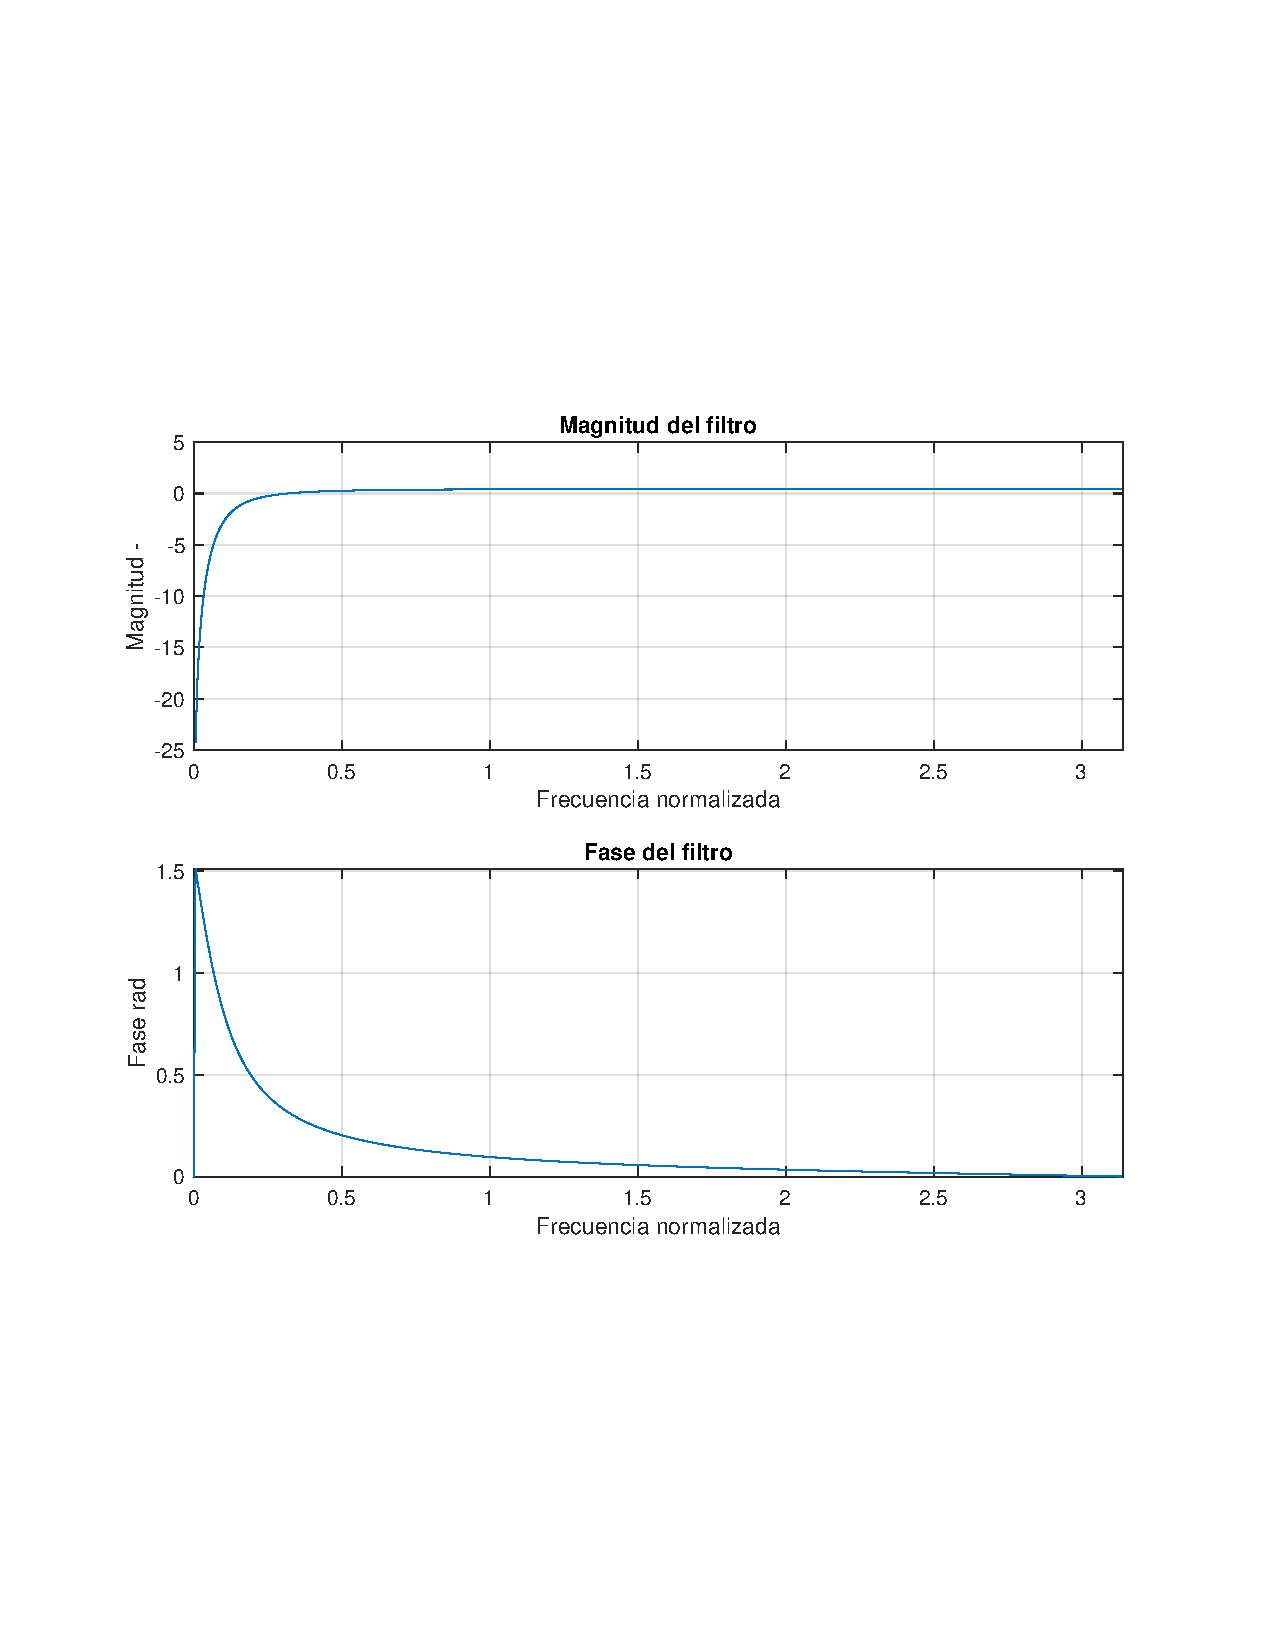
\includegraphics[width=0.6\textwidth,clip, trim = {1.9cm 6.8cm 2.3cm 7cm}]{../plots/1_mag_phase.pdf}
			\caption{Respuesta en magnitud y fase para el filtro}
		\end{figure}
		
		Se procede a evaluar la función \ref{eq:1_filter_transfer_function}, para $\omega = pi$:
		
		\begin{equation}
			H(\pi) = \frac{e^{j\pi} - 1}{e^{j\pi} - 0.9} = \frac{-2}{-1,9} \approx 1.0526
			\label{eq:1_filter_pi}
		\end{equation}
		
		Para normalizar la respuesta del filtro, para $\omega = \pi$, basta con hacer que para esta frecuencia el filtro tenga ganancia unitaria, por lo que se puede definir la ganancia de normalización:
		\begin{equation}
			G_{n} = \frac{1.9}{2} = 0.95
		\end{equation}
		
		Por lo que se puede reescribir la función de transferencia:
		\begin{equation}
			\hat{H}(z) = G_{n} \cdot H(z) = 0.95 \cdot \frac{z - 1}{z -0.9} 
			\label{eq:1_transfer_function_normal}
		\end{equation}
		
		Llevando la expresión a su forma de ecuación de diferencias:
		\begin{align}
			X(z) \cdot 0.95 ( 1 - z^{-1} ) = Y(z) \cdot (1 - 0.9 z^{-1}) \\
			y(z) = 0.9 \cdot y\left[ n - 1 \right] + 0.95 \left( x\left[ n - 1 \right] - x\left[n \right] \right)
		\end{align}
		
		\textcolor{red}{TERMINAR DEMOSTRACIONES - VERIFICAR}
		
		 Considere ahora, que se tiene como entrada del filtro definido en \ref{eq:1_transfer_function_normal}:
		 \begin{equation*}
		 	x[n] = 2 \cdot cos \left( \frac{\pi}{6}n + \frac{\pi}{4} \right)
		 \end{equation*}
		 
		Como se sabe, la expresión tiene una única frecuencia fundamental en $\pm \pi/6$. De esta forma, para el filtro diseñado en el punto anterior, basta evaluar únicamente el efecto de la atenuación y desfase para la frecuencia de la señal de entrada. De esta forma:
		\begin{align}
			|H(\pi/6)| = 0.95 \cdot \left| \frac{e^{j\pi/6} - 1}{e^{j\pi/6} - 0.9} \right| = 0.9812 \\
			\angle H(\pi/6) = arctan\left( 0.95 \cdot \frac{e^{j\pi/6} - 1}{e^{j\pi/6} - 0.9} \right) = 0.1940~\text{rad} 
		\end{align}
		
		De esta forma, se puede obtener la salida:
		\begin{equation}
			y[n] = \sqrt(2) \cdot 0.9812 \cdot cos \left( \frac{\pi n}{6} + \frac{\pi}{4} + 0.1940 \right)
		\end{equation}
		
	\subsection{Filtraje señal electrocardiograma}
		Se pide diseñar un filtro con dos ceros, para el filtraje de una señal ECG muestreada a 200~Hz, con ruido en la banda de 60~Hz. Analizando la señal:
		\begin{figure}[H]
			\center
			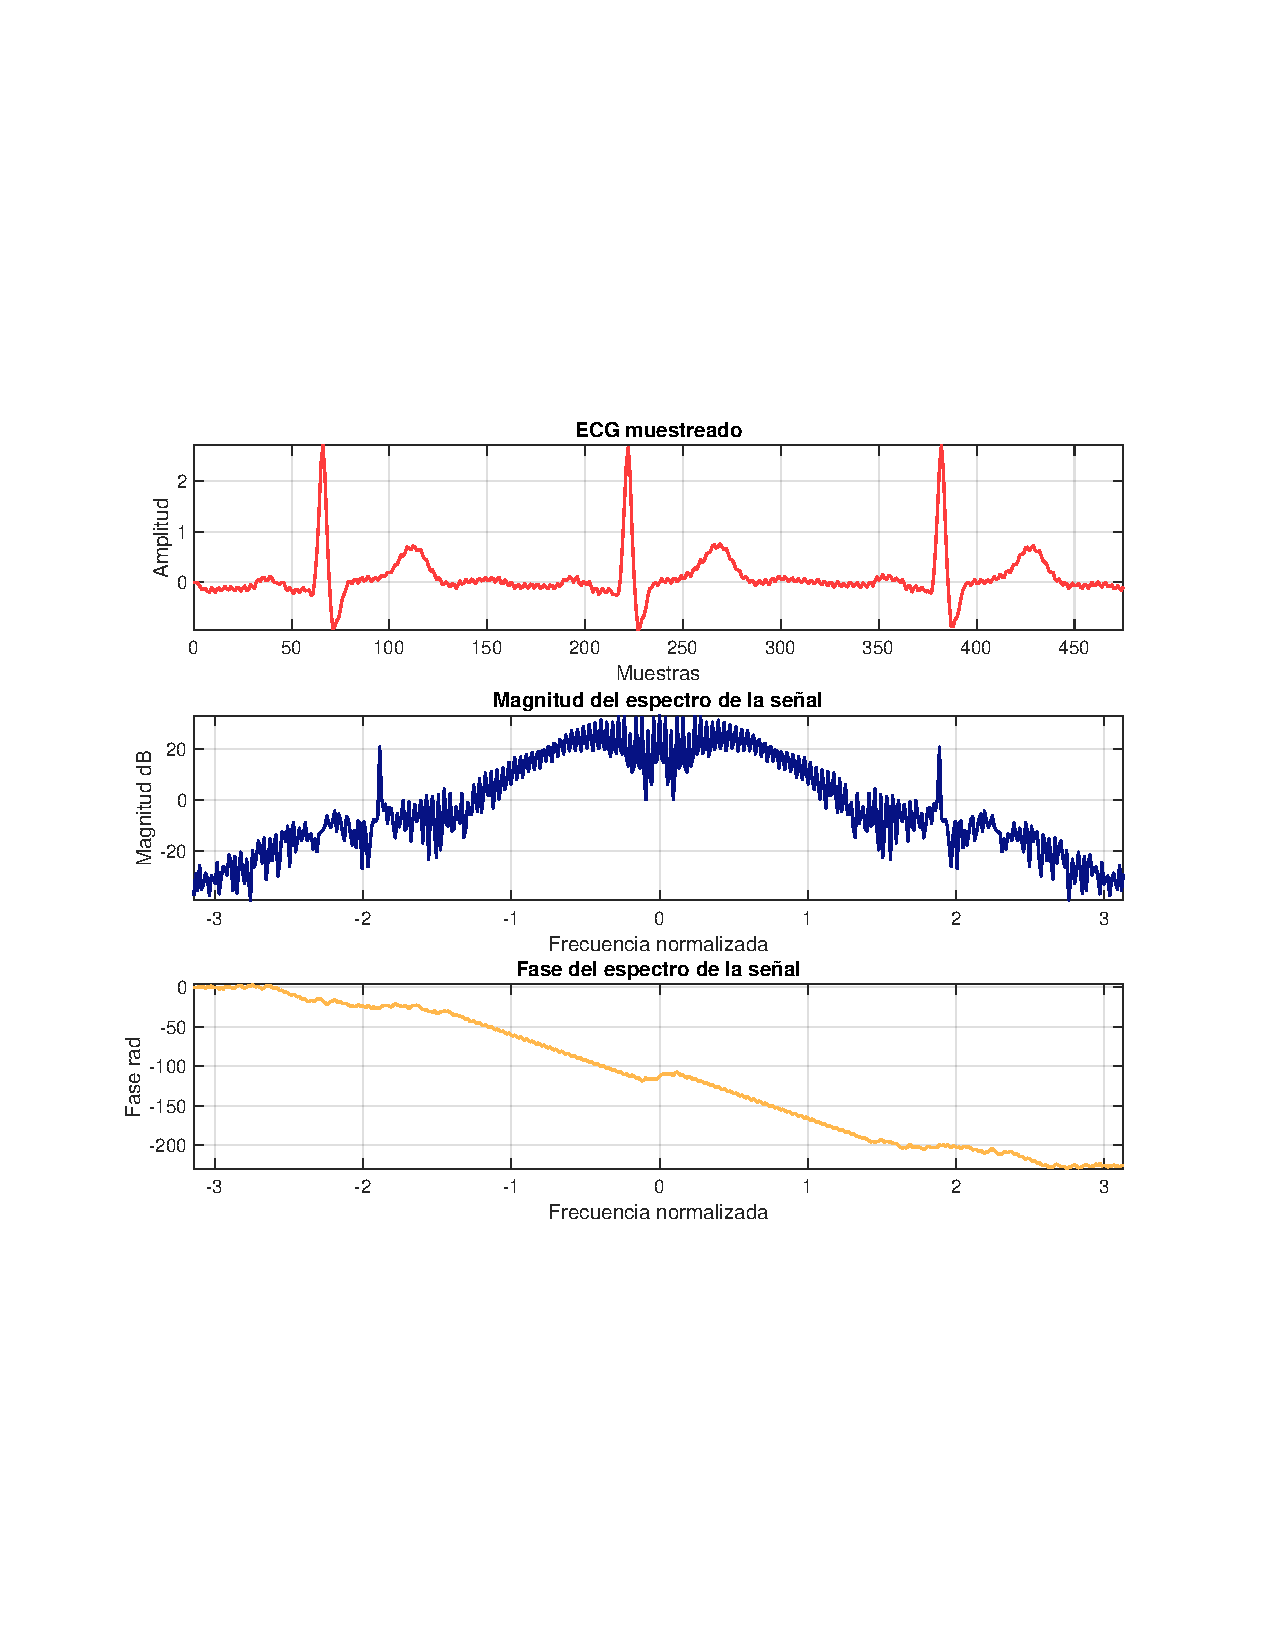
\includegraphics[width=0.6\textwidth,clip, trim = {1.9cm 6.8cm 2.3cm 7cm}]{../plots/ecg_time_freq.pdf}
			\caption{Señal muestreada, en el dominio temporal y de frecuencia}
			\label{fig:ecg_time_freq}
		\end{figure}		
				
		Se puede ver claramente, las bandas de ruido presentes. Se propone la siguiente estructura para el filtro:
		\begin{align}
			\omega_{r} = \frac{2\pi 60}{200} = 0.6\pi \\
			H(z) = \frac{(z-e^{j\omega_r})(z-e^{-j\omega_r})}{z^{2}} = \frac{z^{2} + 2cos(\omega_{r}) + 1}{z^{2}}
		\end{align}
		
		Realizando la implementación en \textsc{Matlab}, se puede obtener la magnitud y fase del filtro:
		\begin{figure}[H]
			\center
			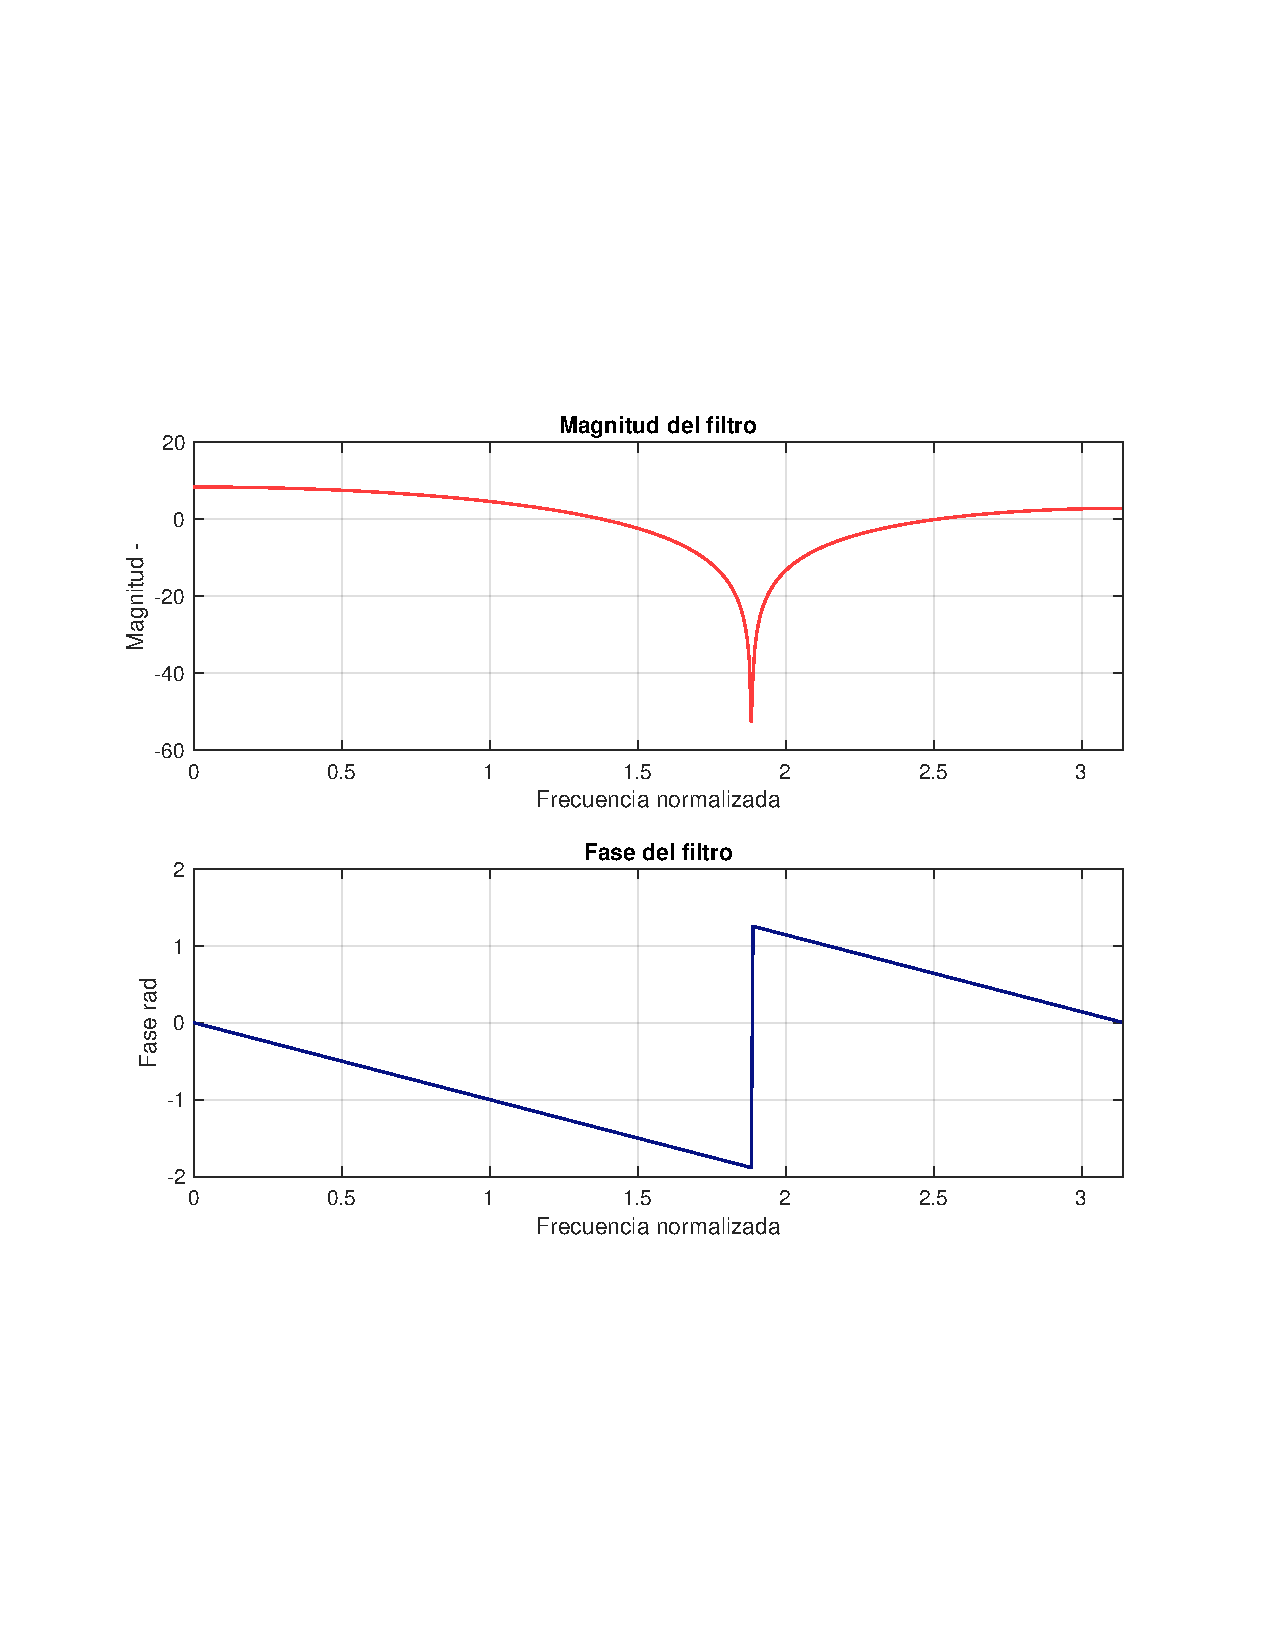
\includegraphics[width=0.6\textwidth,clip, trim = {1.9cm 6.8cm 2.3cm 7cm}]{../plots/ecg_poles_0.pdf}
			\caption{Respuesta en magnitud y fase para el filtro}
			\label{fig:mag_phase_p_0}
		\end{figure}
		
		A partir de las respuestas del filtro, se puede ver que en términos de magnitud, tiene un rechazo relativamente lento, con la banda de paso no plana. En términos de la fase, se puede ver que se tiene un desfase lineal deseable. Aplicando el filtro a la señal:
		
		\begin{figure}[H]
			\center
			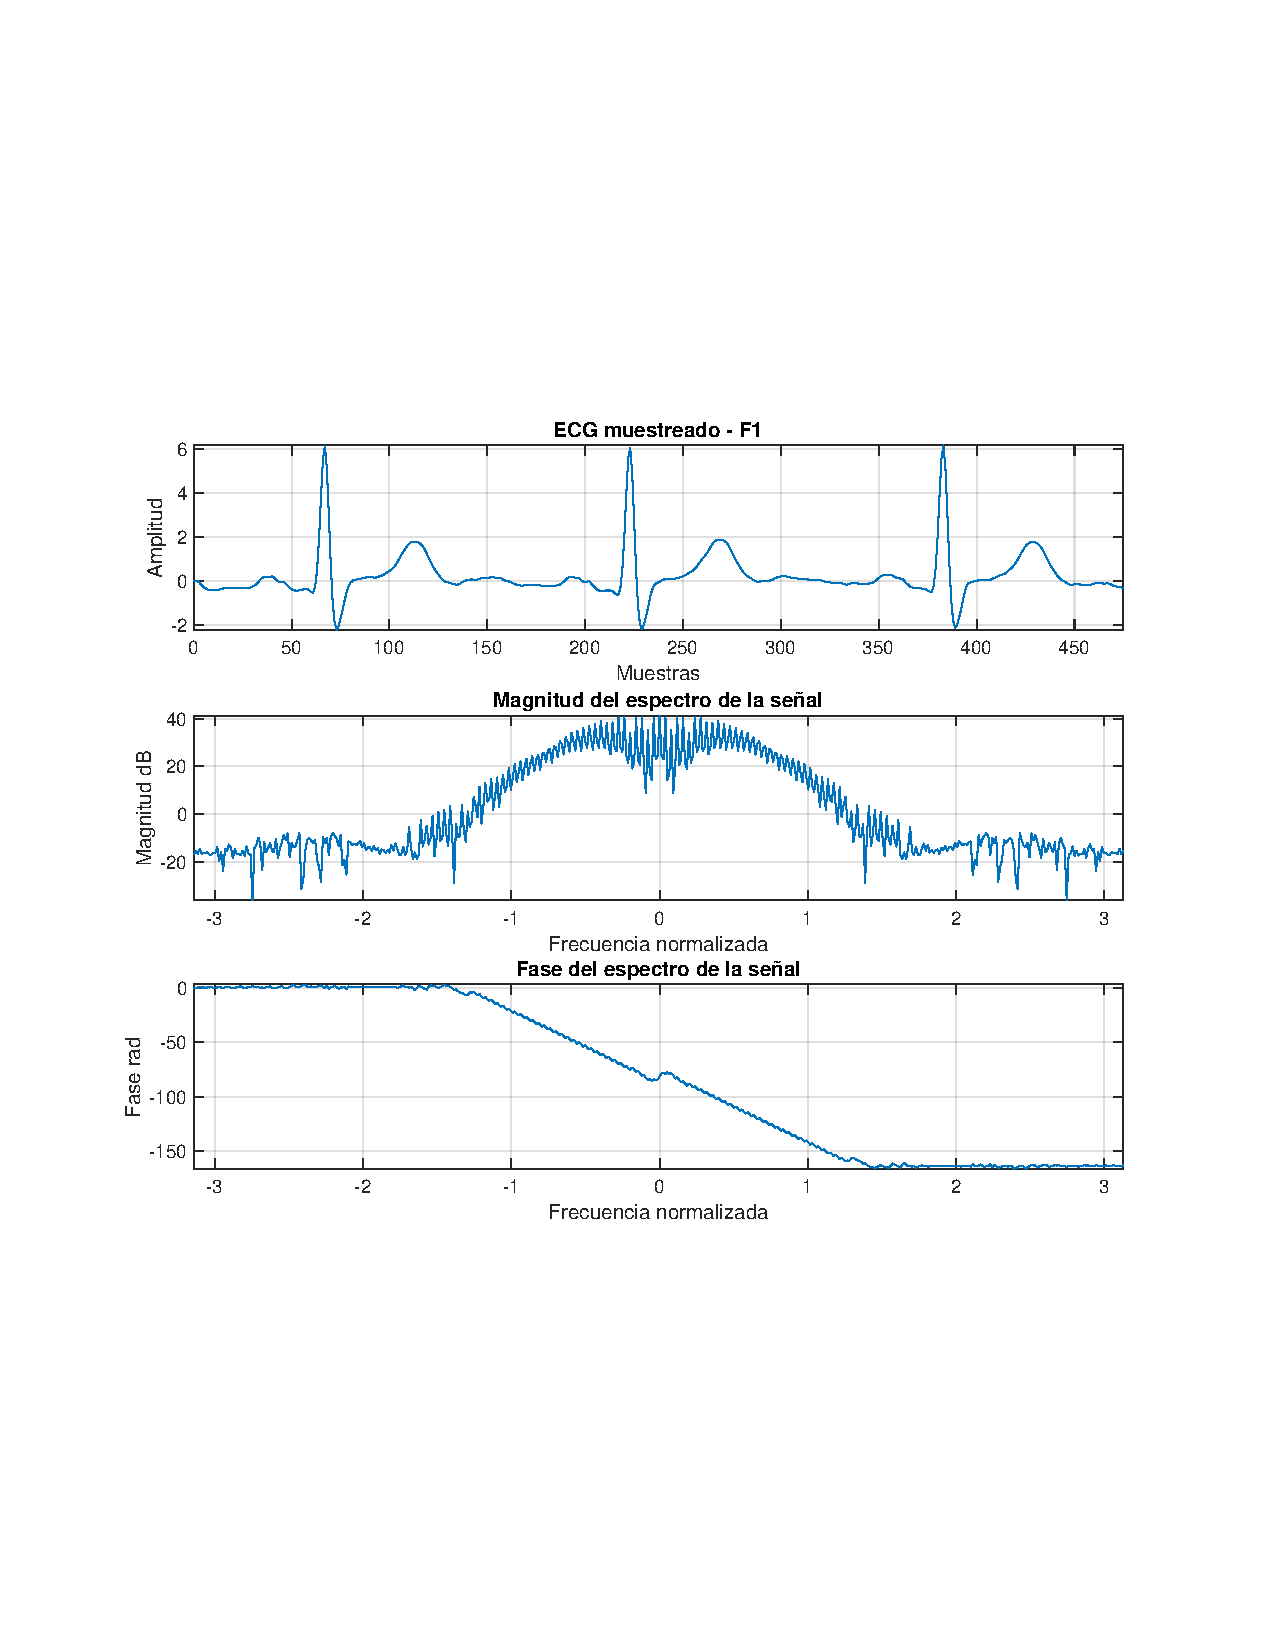
\includegraphics[width=0.6\textwidth,clip, trim = {1.9cm 6.8cm 2.3cm 7cm}]{../plots/ecg_poles_0_filtered.pdf}
			\caption{Resultado del filtraje de la señal}
			\label{fig:ecg_filtered_0}
		\end{figure}
		
		Se puede ver que el proceso de filtrado ha sido exitoso, permitiendo remover la banda con ruido de la señal. Se puede ver una cierta \textit{amplificación} de ciertas bandas, dada la forma no plana del filtro, el espectro se tendió a \textit{curvar}. En términos de fase, se puede ver que el efecto del filtro sobre ésta, es el esperado, dada la fase lineal del filtro. Realizando una comparación directa de ambas señales:
		\begin{figure}[H]
			\center
			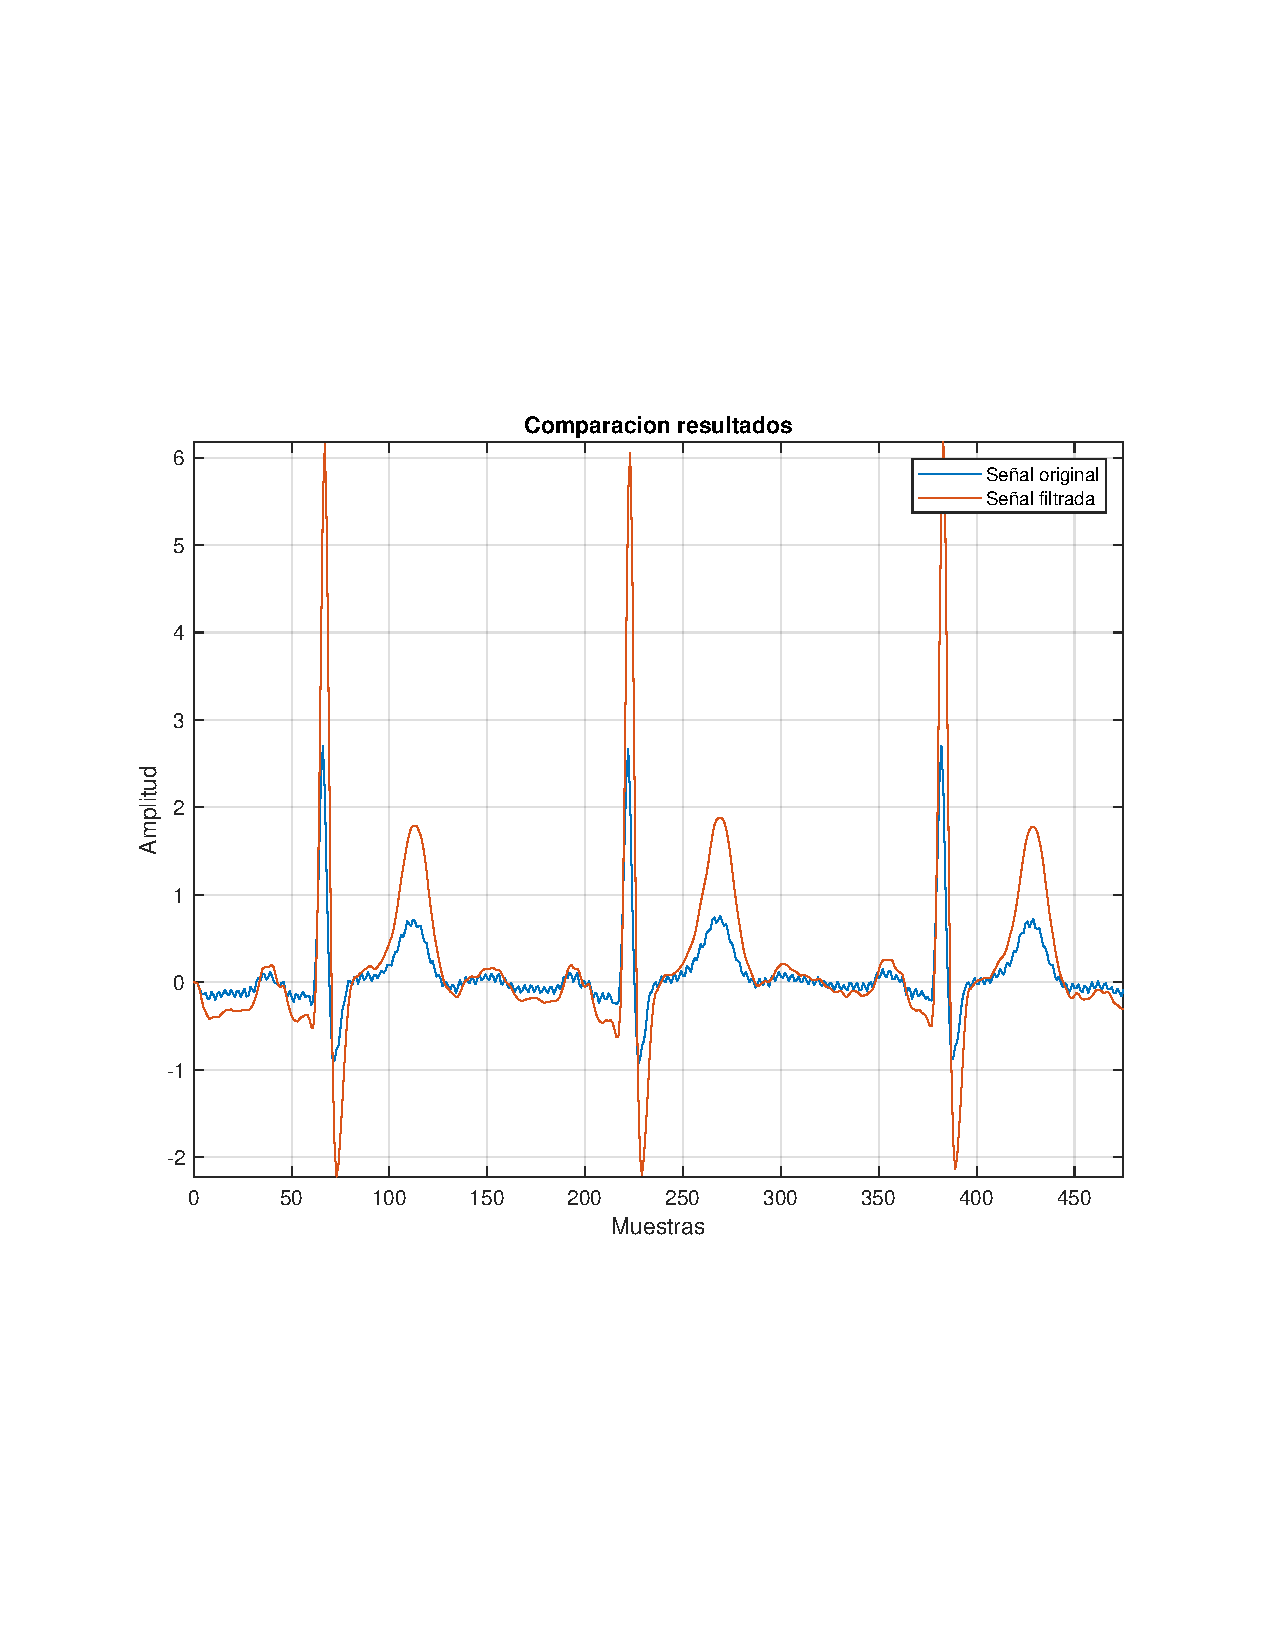
\includegraphics[width=0.6\textwidth,clip, trim = {1.9cm 6.8cm 2.3cm 7cm}]{../plots/egc_f_0_comparative.pdf}
			\caption{Comparación de las señales}
			\label{fig:ecg_filtered_0_comparative}
		\end{figure}
		
		Considere ahora, que se añaden dos polos a la frecuencia de rechazo, con un radio $r \in [0,8  - 0,99]$. A partir de esto, se escogen tres valores para $r = 0.8, r = 0.9, r = 0.99$. Implementando los filtros y comparando su respuesta en magnitud y frecuencia:
		\begin{figure}[H]
			\center
			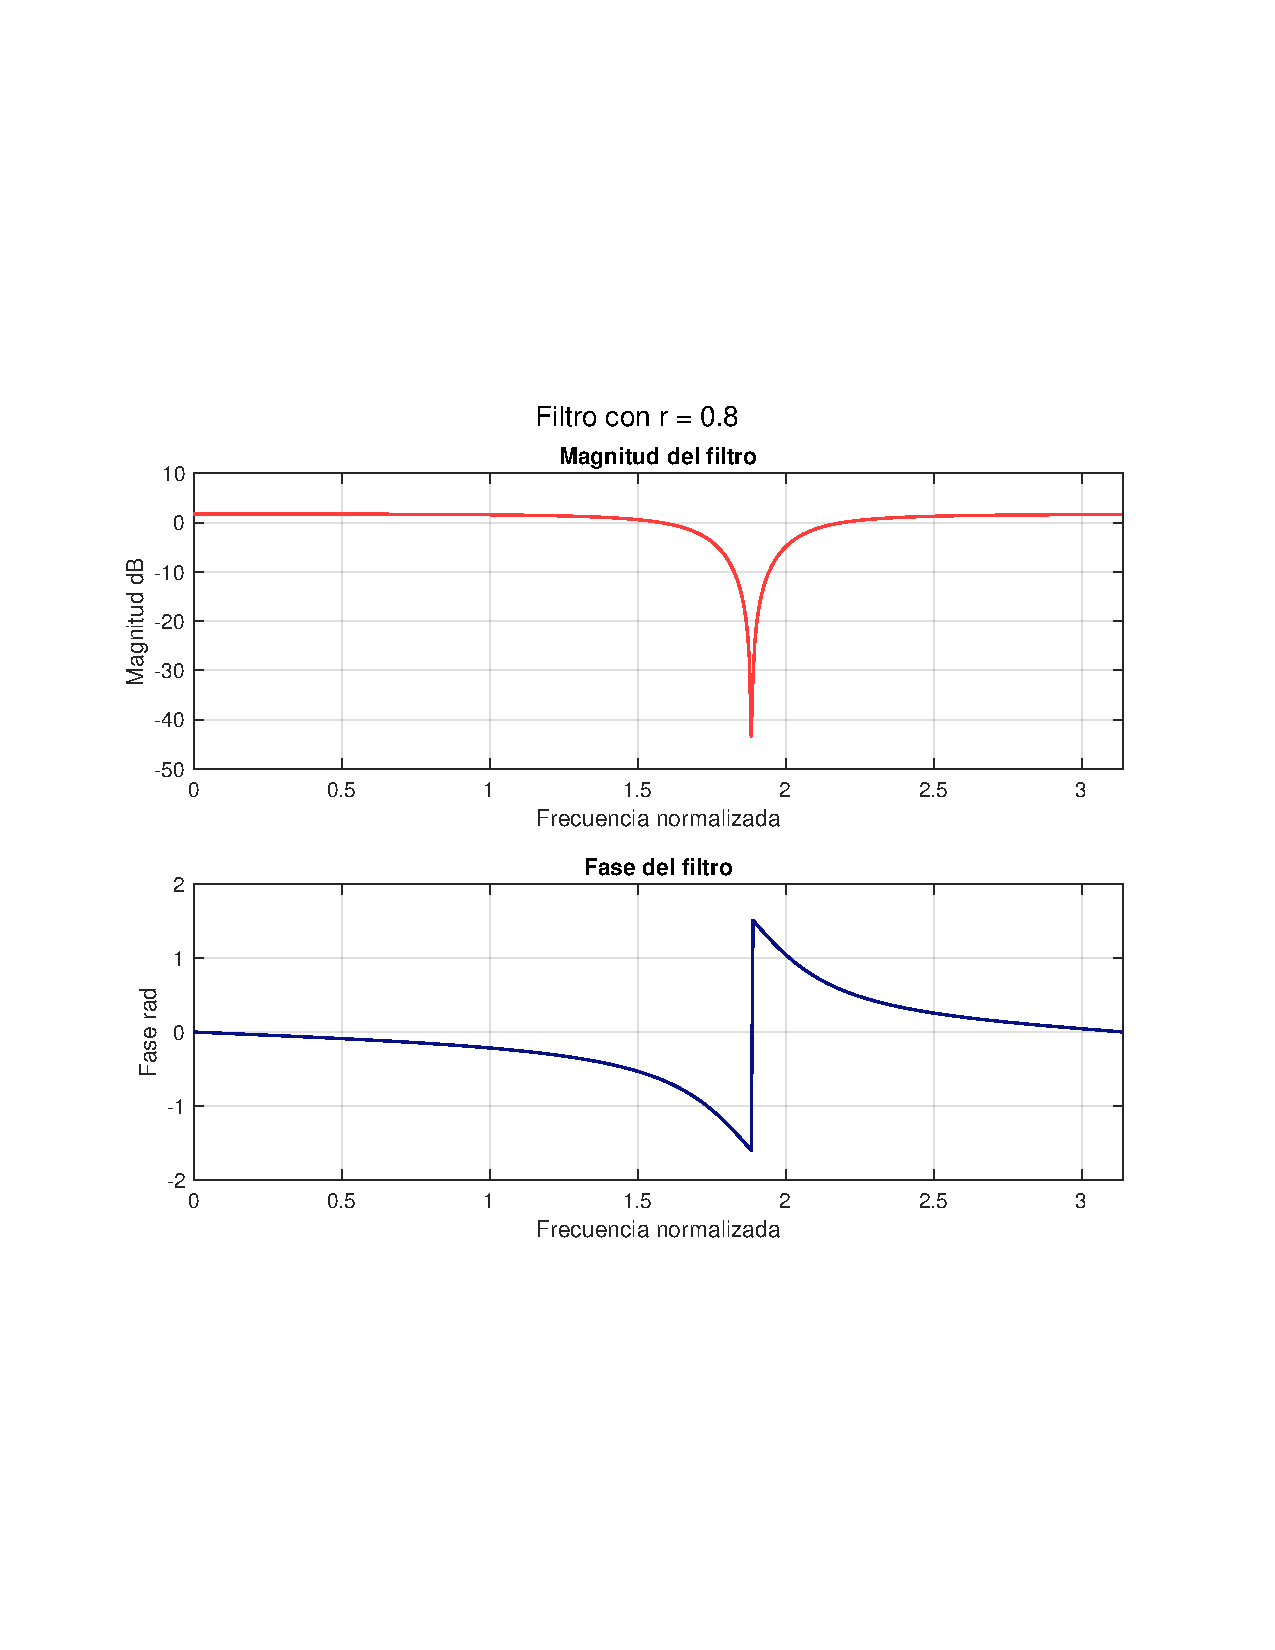
\includegraphics[width=0.6\textwidth,clip, trim = {1.9cm 6.8cm 2.3cm 7cm}]{../plots/ecg_poles_208.pdf}
			\caption{Respuesta del filtro, para r = 0.8}
			\label{fig:ecg_filter_r_08}
		\end{figure}

		\begin{figure}[H]
			\center
			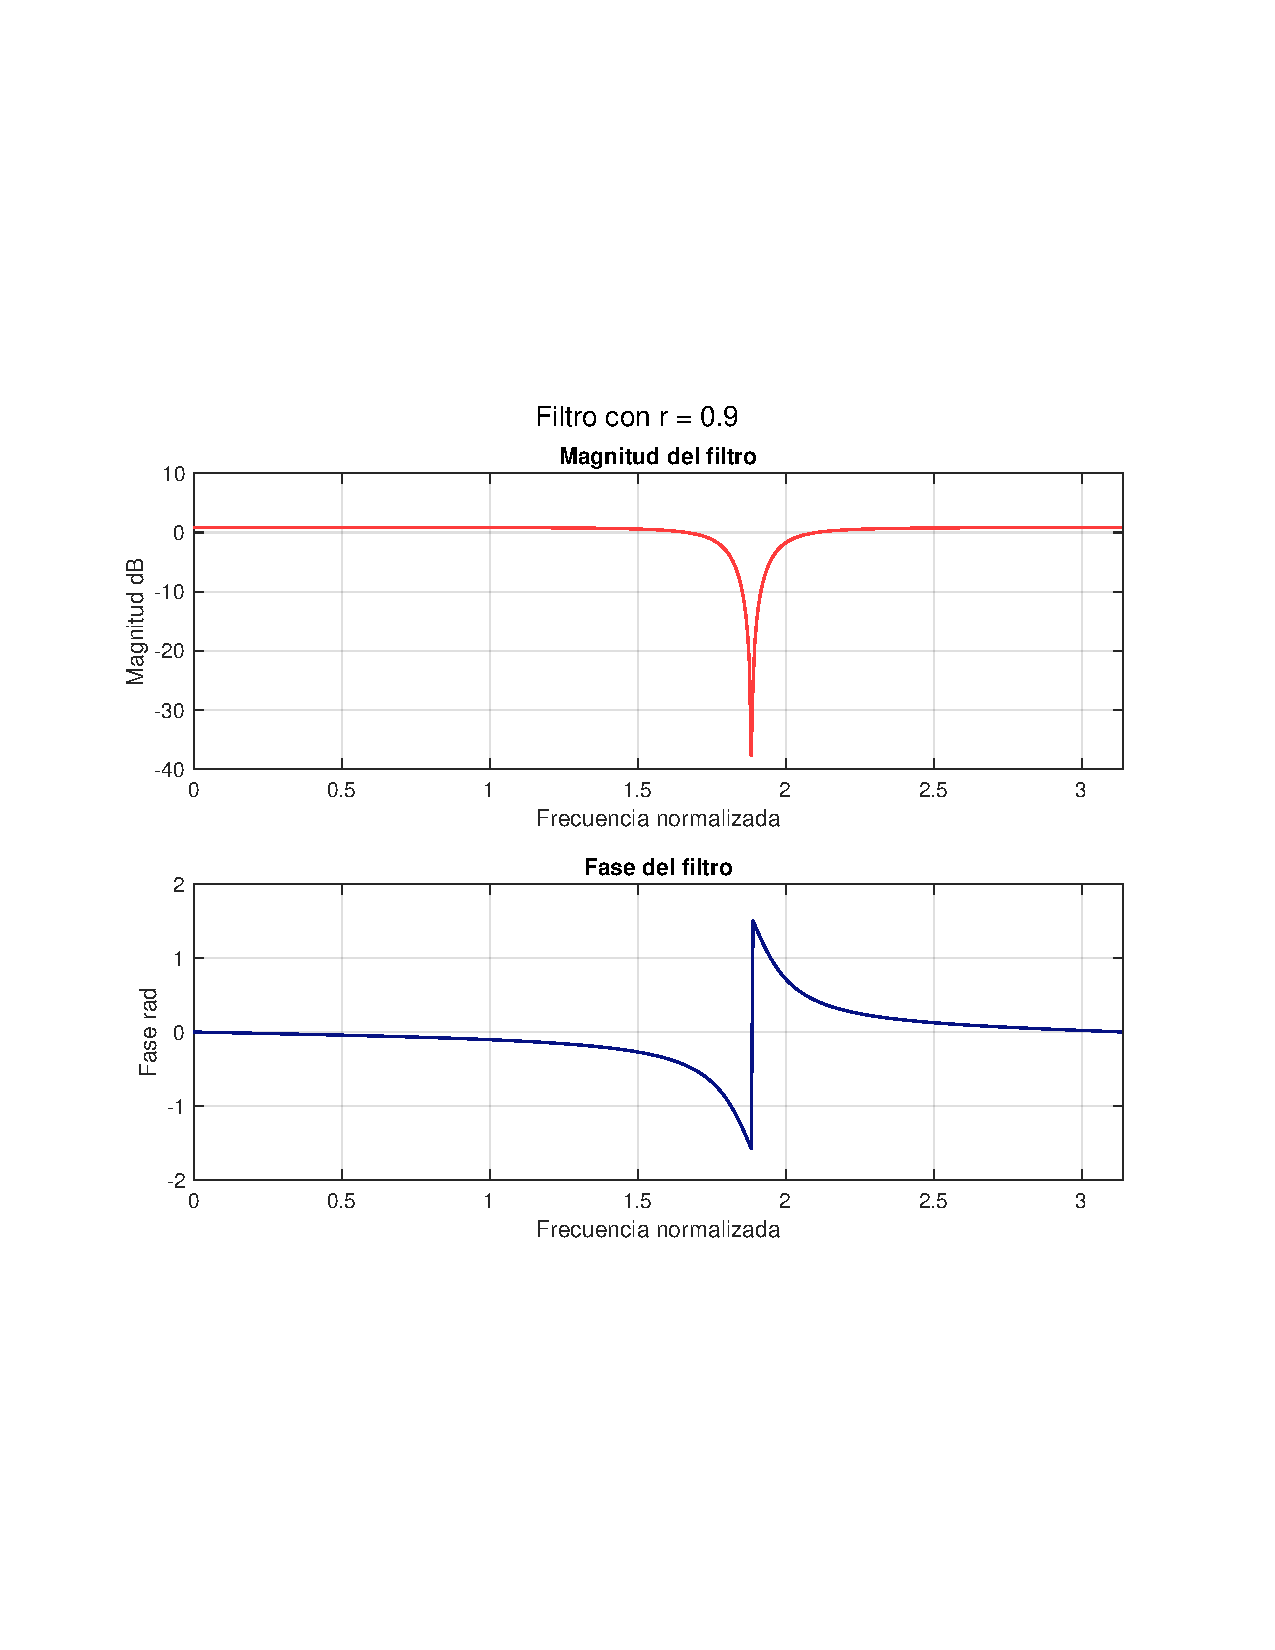
\includegraphics[width=0.6\textwidth,clip, trim = {1.9cm 6.8cm 2.3cm 7cm}]{../plots/ecg_poles_209.pdf}
			\caption{Respuesta del filtro, para r = 0.9}
			\label{fig:ecg_filter_r_09}
		\end{figure}		
		
		\begin{figure}[H]
			\center
			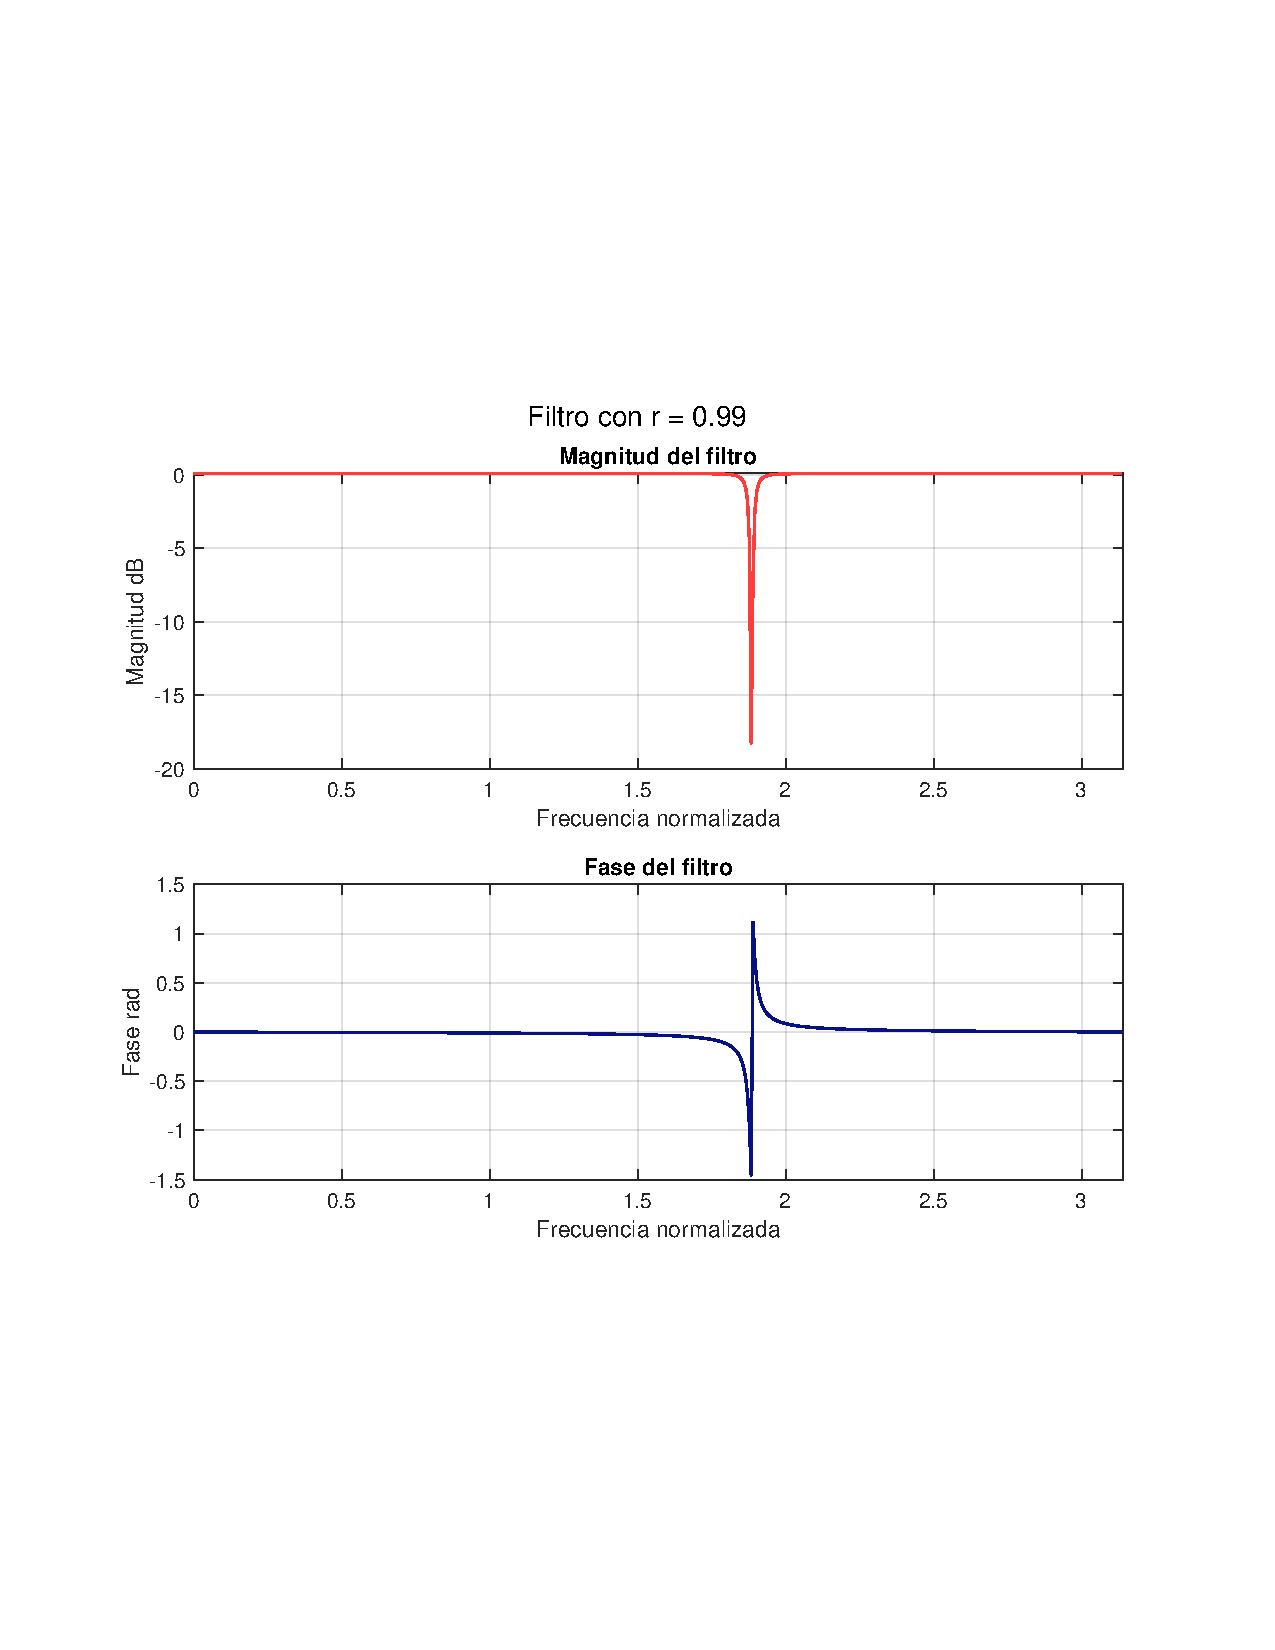
\includegraphics[width=0.6\textwidth,clip, trim = {1.9cm 6.8cm 2.3cm 7cm}]{../plots/ecg_poles_2099.pdf}
			\caption{Respuesta del filtro, para r = 0.99}
			\label{fig:ecg_filter_r_099}
		\end{figure}
		
		A partir de estos resultados, se puede comprobar que a medida que el valor de $r$, se acerca al círculo unitario, la banda de rechazo se hace mas angosta, acercándose lo más posible a la respuesta ideal de un filtro \textit{notch}, sin embargo, esta mejora en el rechazo del filtro, trae consigo que la fase, que inicialmente era ``perfectamente'' lineal, se empieza a curvar en torno a la banda de rechazo. Por lo tanto al construir el filtro, se debe tener en cuenta la aplicación final, dado que determinará si es factible tener un mejor rechazo a costa de una fase no lineal. La mejora en el rechazo del filtro, se puede explicar, si consideramos que un cero anula la función de transferencia, mientras que un polo la \textit{indefine}, por lo que entre mas cerca esté el polo del cero, la recuperación de la anulación en el espectro será mejor y más rápida, dando un filtro más selectivo. Otro punto a destacar, es que a medida que el valor de r se acerca al círculo unitario, la respuesta en magnitud se hace más plana, eliminando la curvatura del espectro que se tenía para el filtro con polos en cero, figura \ref{fig:mag_phase_p_0}. Tomando el caso para $r = 0.99$, se filtra la señal ECG entregada, obteniéndose el siguiente resultado:
		
		\begin{figure}[H]
			\center
			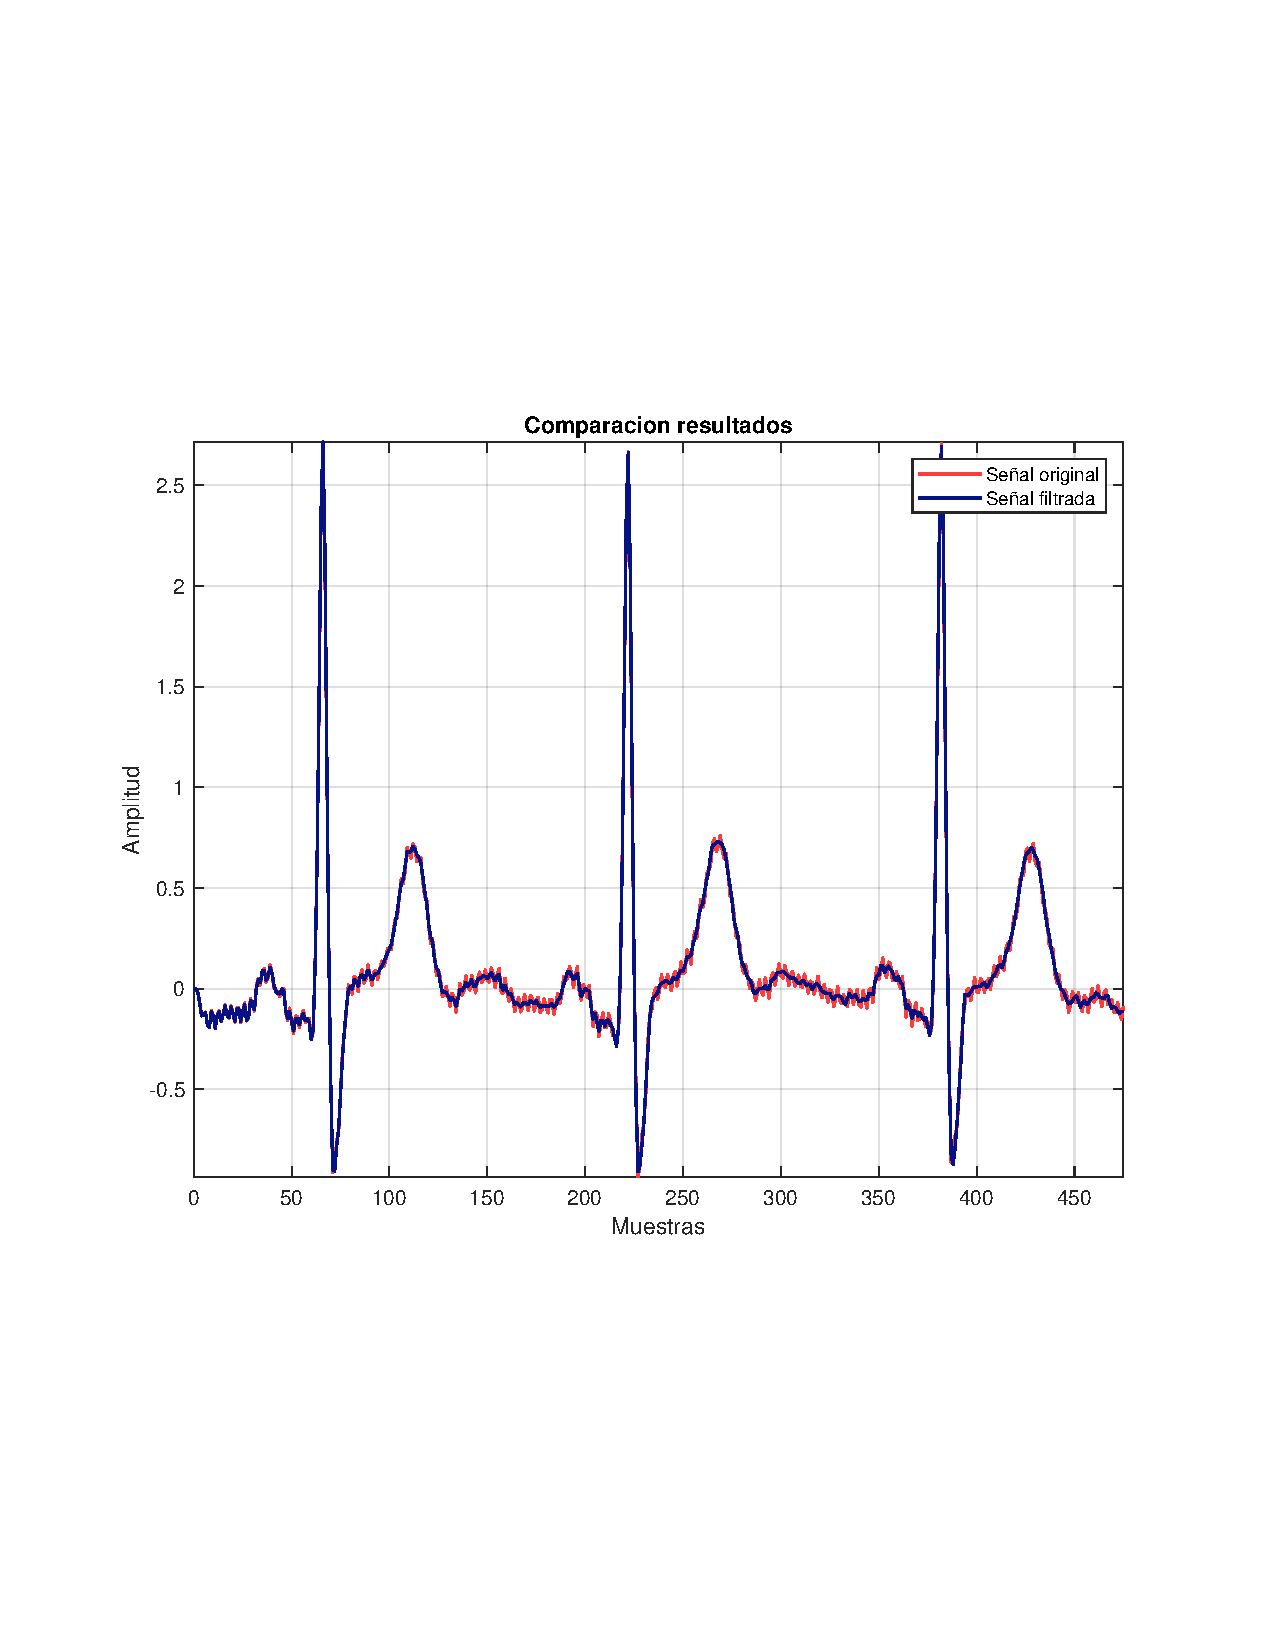
\includegraphics[width=0.6\textwidth,clip, trim = {1.9cm 6.8cm 2.3cm 7cm}]{../plots/egc_f_2_comparative.pdf}
			\caption{Resultado de filtraje, para r = 0.99}
			\label{fig:ecg_filter_r_099_result}
		\end{figure}
		
		A partir de esto, se puede comprobar, que se tiene un mejor filtrado de la señal, y que el efecto causado por la fase no lineal, no es apreciable. La respuesta más plana en frecuencia, permite que el filtro siga de manera más cercana la señal original, sin tener efectos de amplificación, como en el caso de polos en cero. Por lo que para esta aplicación el filtro diseñado para $r = 0.99$ es una buena solución. 
		
	\subsection{Filtrado de ECG con variación DC}
		A partir de la señal \texttt{ecg\_lfn}, se deben construir filtros de orden $n = \{2,8 \}$ con frecuencias $f = \{0.5 \quad 5\}$~Hz. Se procede a implementar los filtros pedidos y analizar su respuesta en frecuencia:
		
		\begin{figure}[H]
			\center
			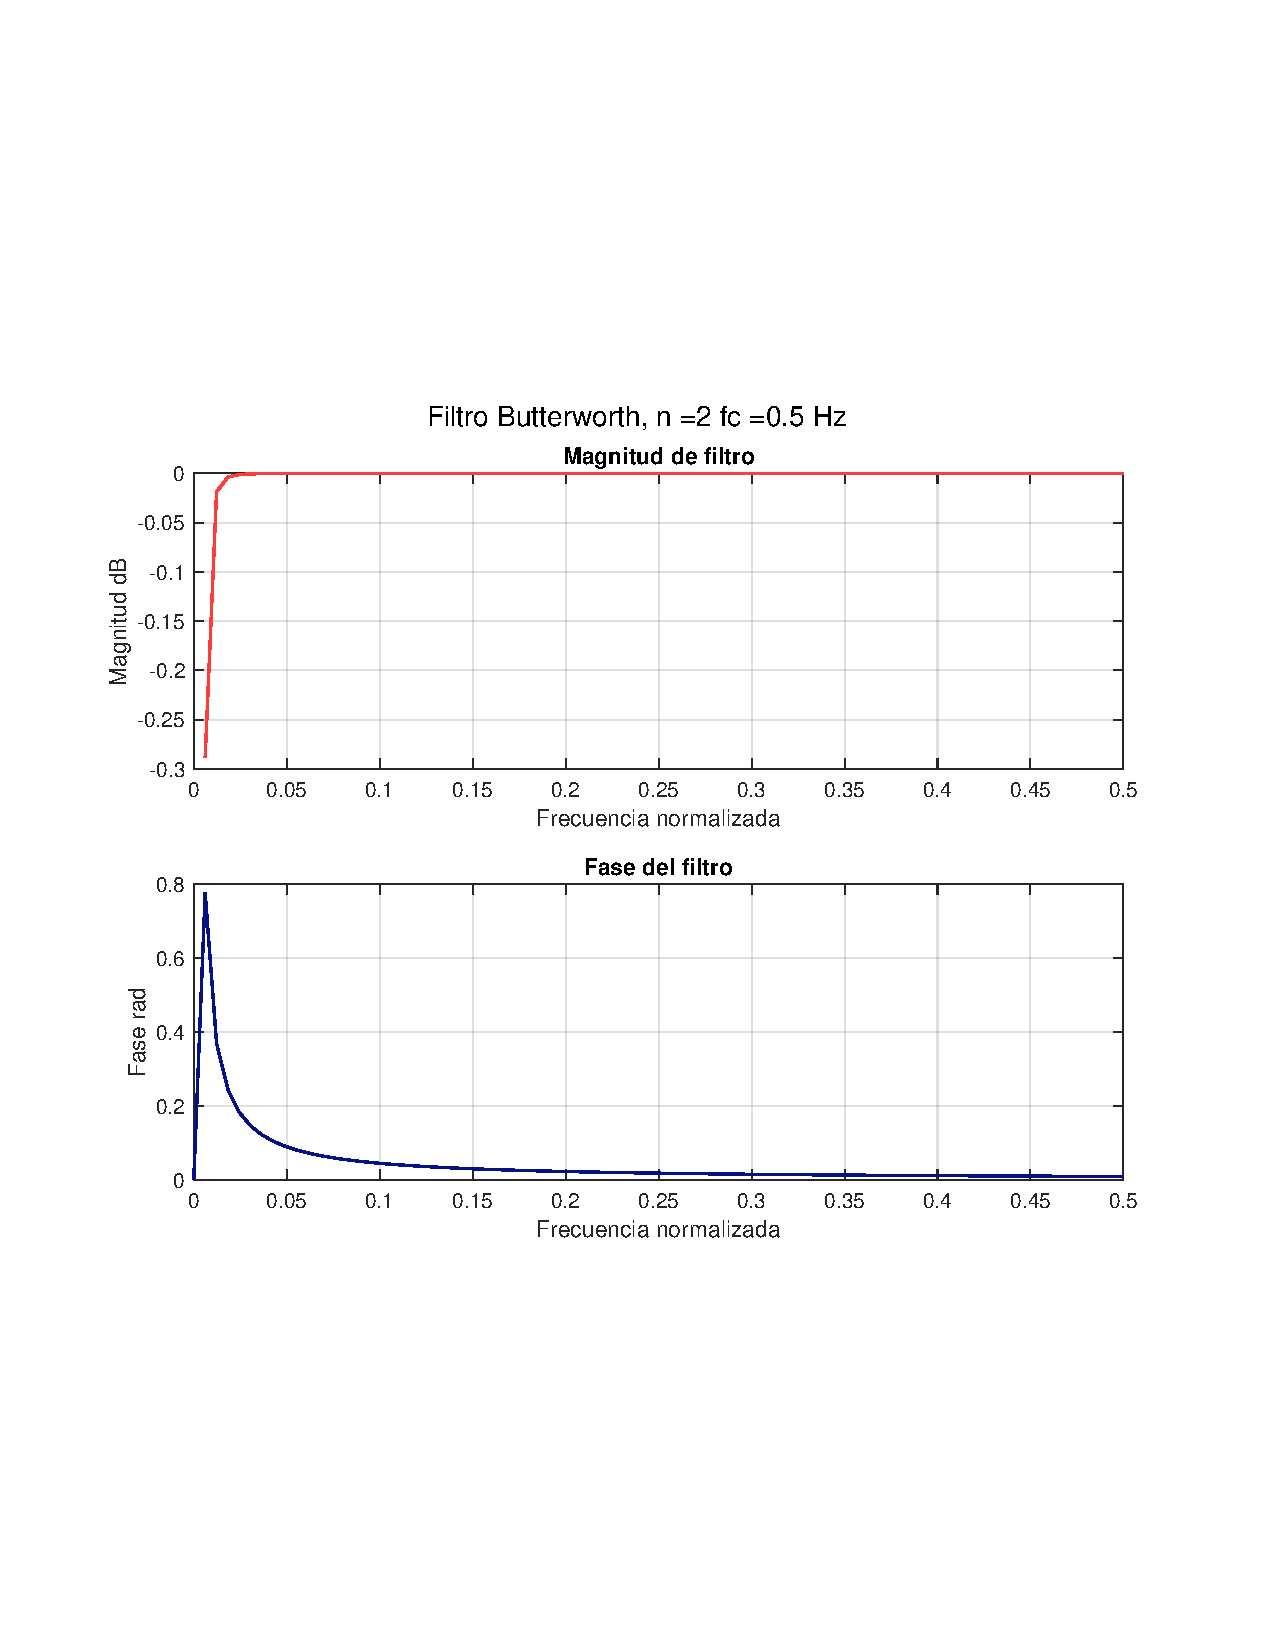
\includegraphics[width=0.6\textwidth,clip, trim = {1.9cm 6.8cm 2.3cm 7cm}]{../plots/1_c_filter_butter_2_freq_05.pdf}
			\caption{Respuesta en frecuencia de filtro de orden n = 2, fc = 0.5}
			\label{fig:1_c_n2_fc_05}
		\end{figure}

		\begin{figure}[H]
			\center
			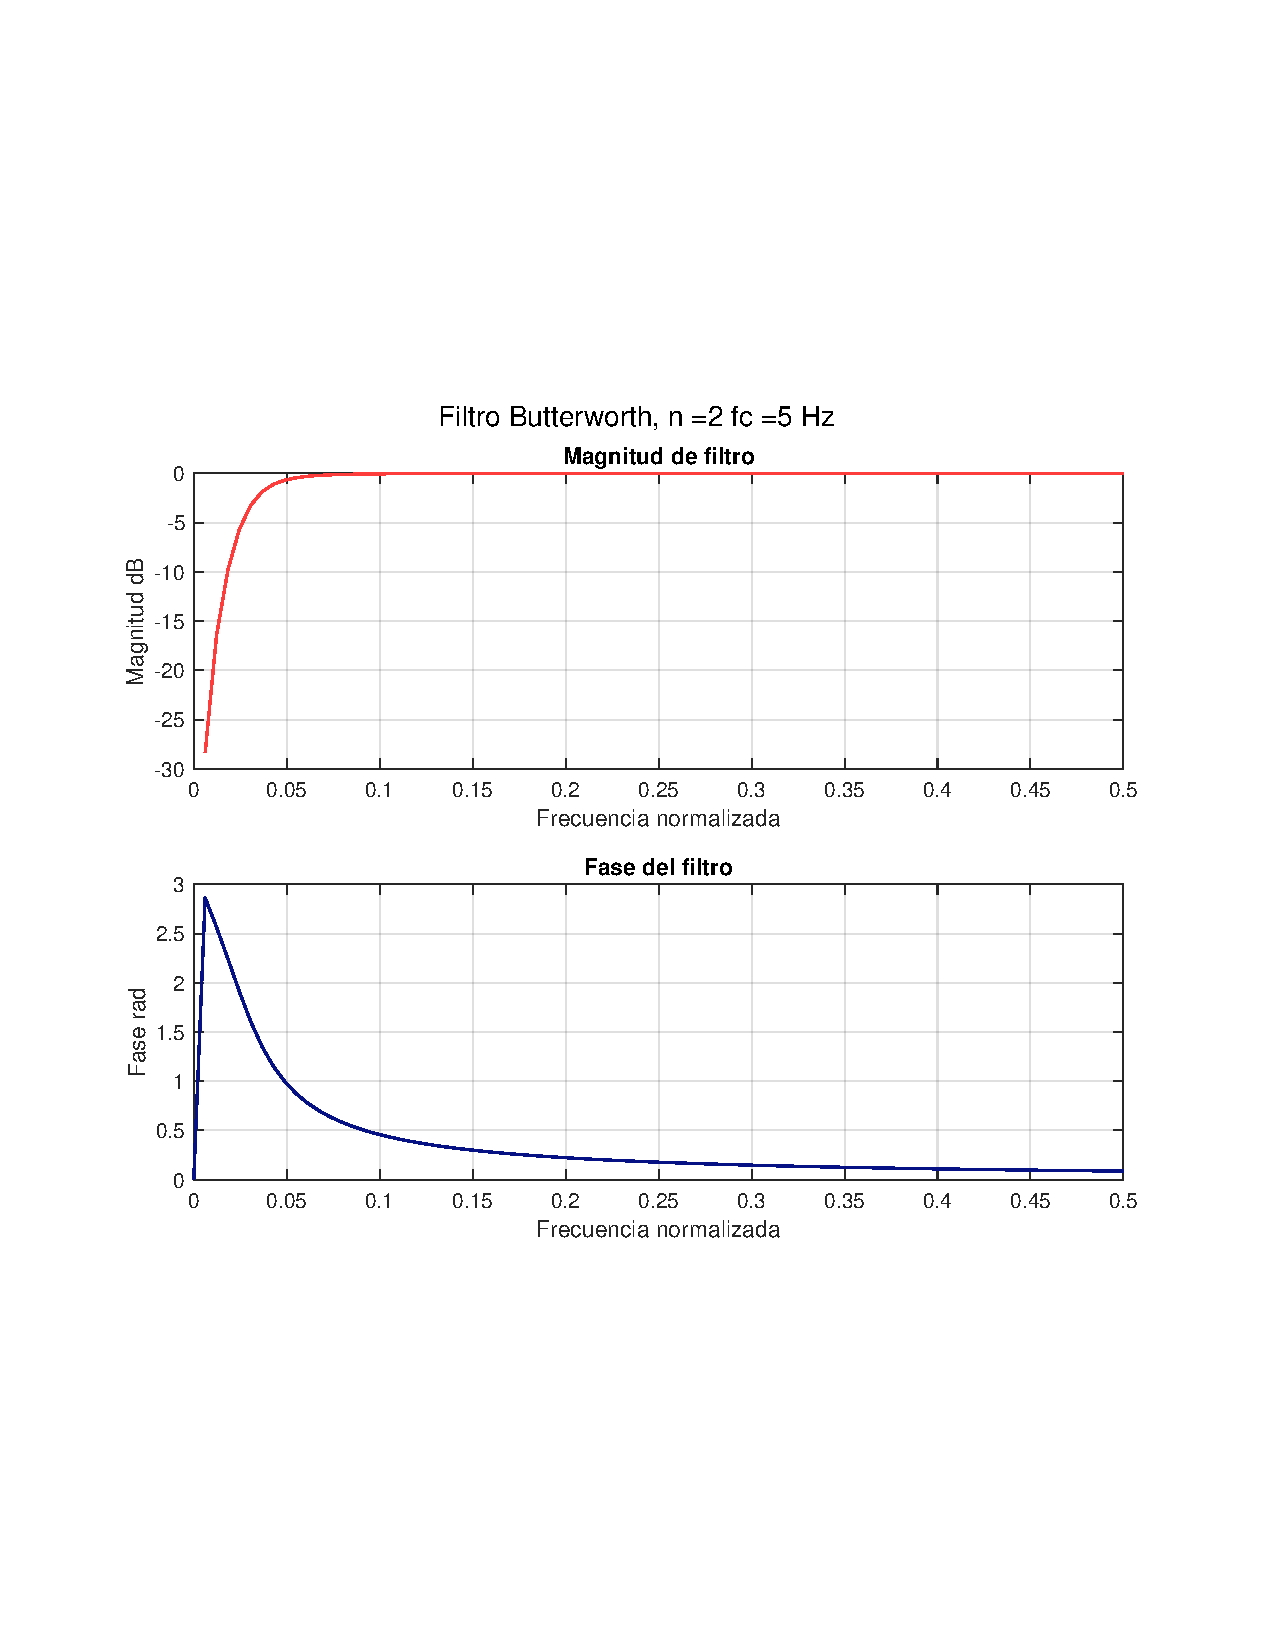
\includegraphics[width=0.6\textwidth,clip, trim = {1.9cm 6.8cm 2.3cm 7cm}]{../plots/1_c_filter_butter_2_freq_5.pdf}
			\caption{Respuesta en frecuencia de filtro de orden n = 2, fc = 5}
			\label{fig:1_c_n2_fc_5}
		\end{figure}	

		\begin{figure}[H]
			\center
			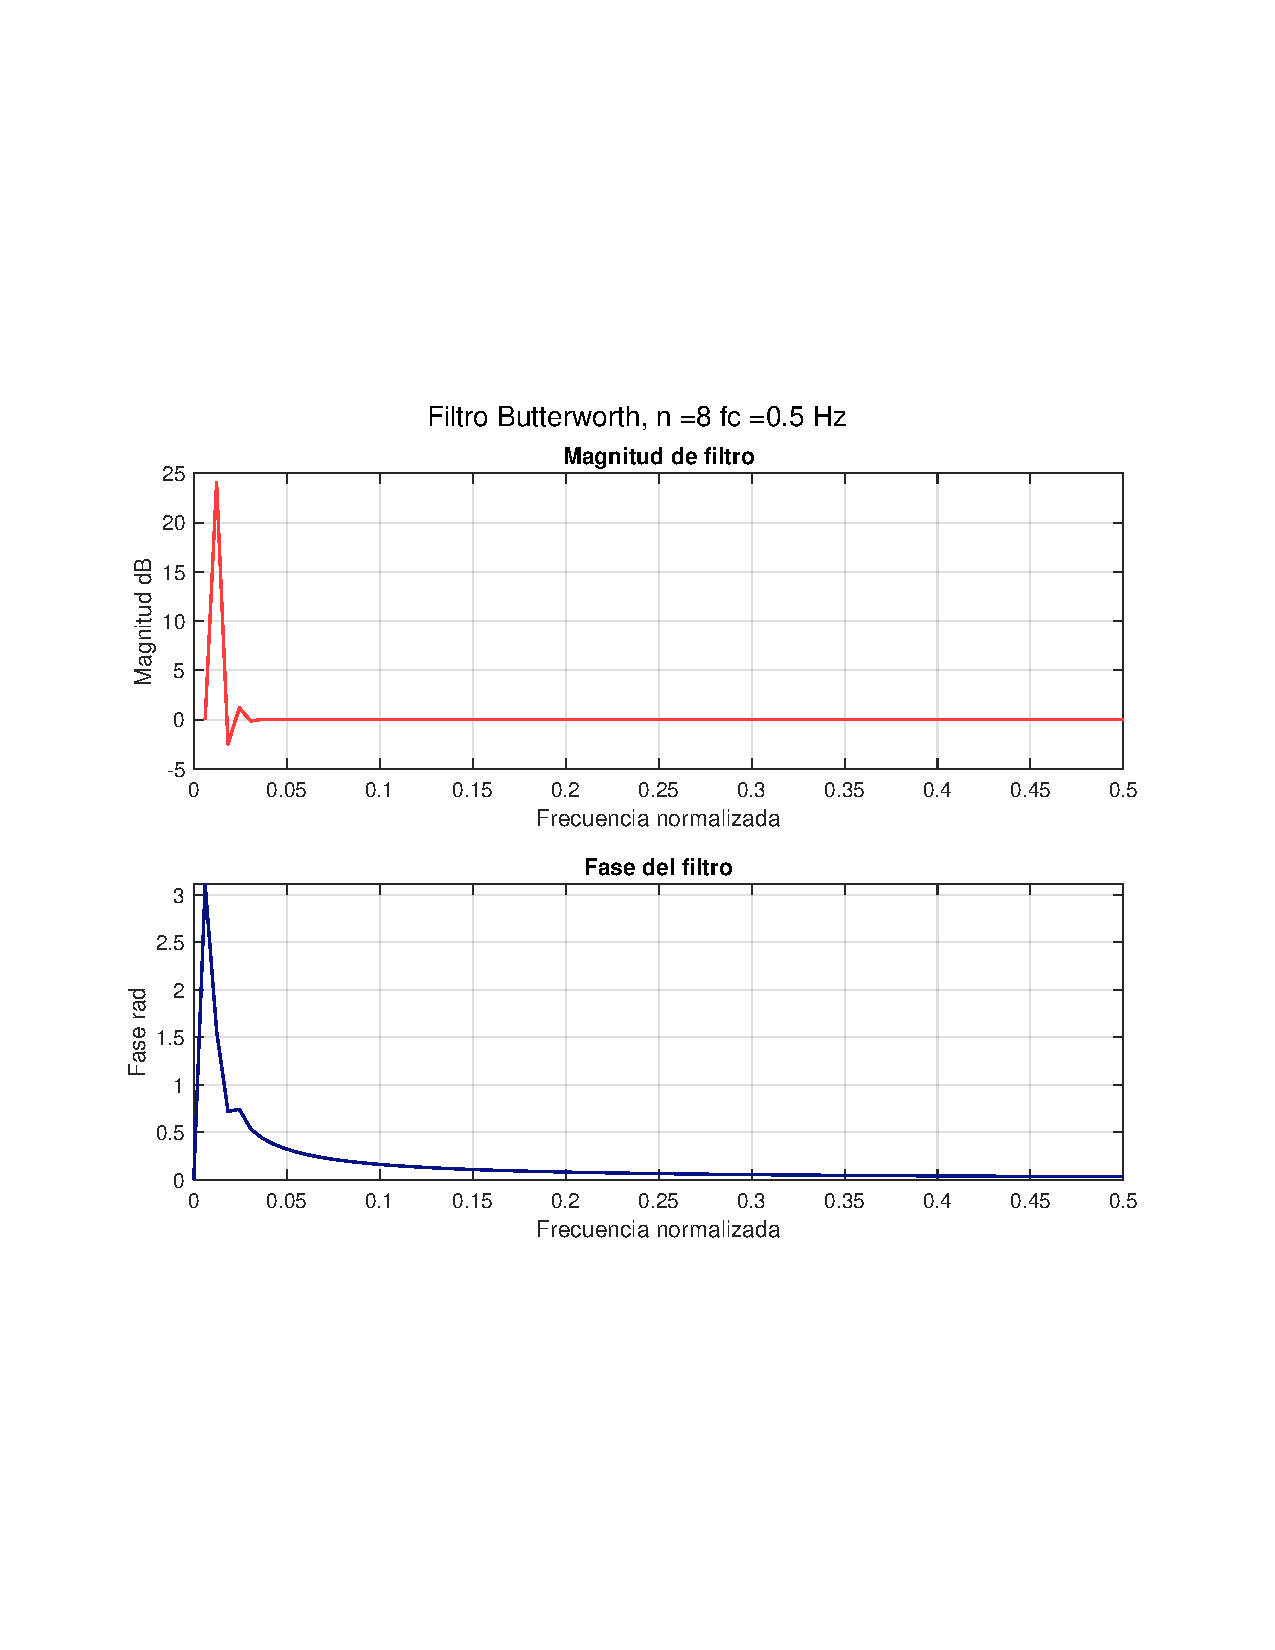
\includegraphics[width=0.6\textwidth,clip, trim = {1.9cm 6.8cm 2.3cm 7cm}]{../plots/1_c_filter_butter_8_freq_05.pdf}
			\caption{Respuesta en frecuencia de filtro de orden n = 8, fc = 0.5}
			\label{fig:1_c_n8_fc_05}
		\end{figure}
		
		\begin{figure}[H]
			\center
			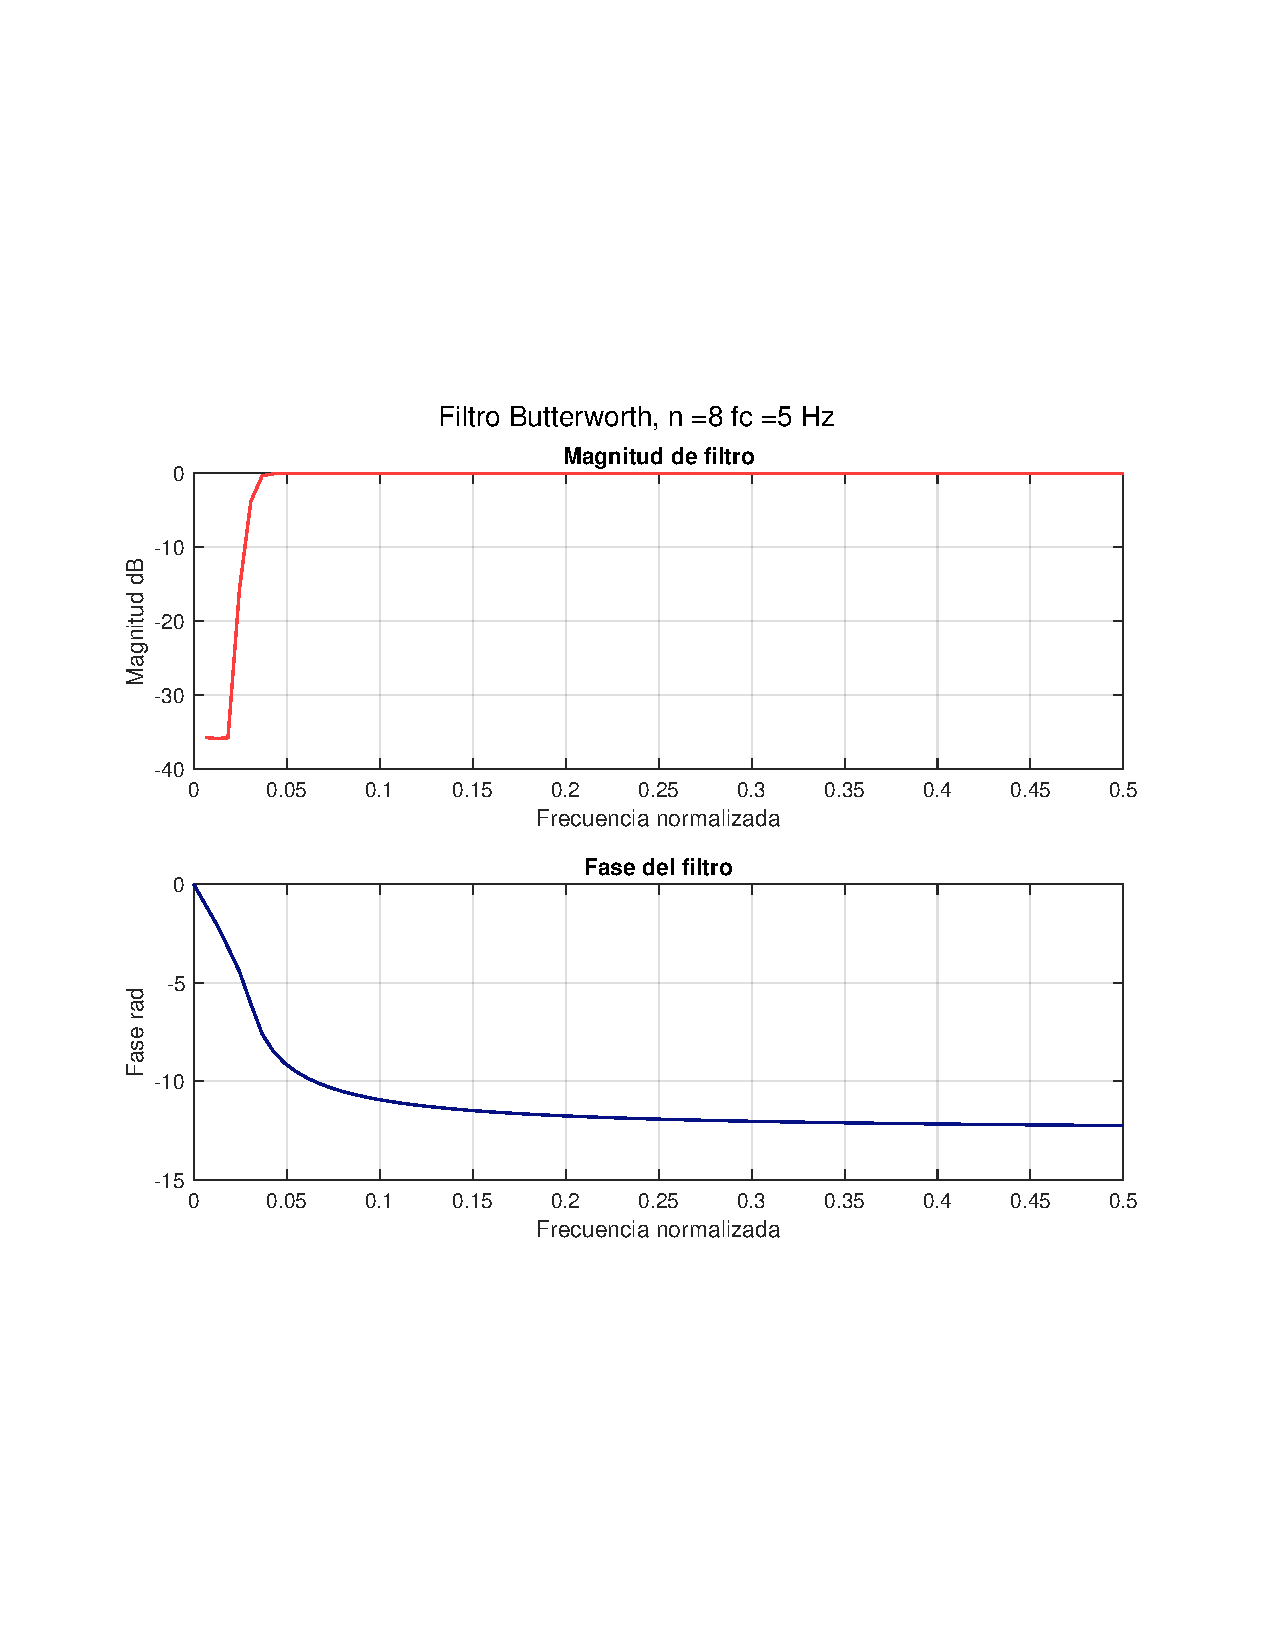
\includegraphics[width=0.6\textwidth,clip, trim = {1.9cm 6.8cm 2.3cm 7cm}]{../plots/1_c_filter_butter_8_freq_5.pdf}
			\caption{Respuesta en frecuencia de filtro de orden n = 8, fc = 5}
			\label{fig:1_c_n8_fc_5}
		\end{figure}
		
		Con la respuesta de los filtros, se puede identificar que para orden pequeño $n = 2$, mover la frecuencia de corte más cerca o lejos de cero, impacta en la capacidad del filtro de rechazar la banda DC, para el caso de $fc = 0.5$, la respuesta es muy similar a un filtro \textit{notch} figura \ref{fig:1_c_n2_fc_05}, sin embargo, la atenuación alcanza aproximadamente 0.3 \textit{dB}, lo cual no es un rechazo considerable. Al mover la frecuencia a $fc = 5$, el filtro es más capaz de rechazar la banda DC figura \ref{fig:1_c_n2_fc_5}, alcanzando un rechazo de 30 \textit{dB}, aproximadamente 100 veces mejor que en el primer caso. Esto, a su vez, trae consigo que la curva de desfase, se extienda, por lo que el filtro con $fc = 5$ tiene un sector de fase no lineal mayor que en el caso de $fc = 0.5$. Para orden mayor, $n = 8$, cuando la frecuencia de corte, es muy cercana a la banda de rechazo, $fc = 0.5$, se tiene que el filtro se vuelve inestable, teniendo una respuesta la cual no es de un filtro rechaza banda, como se ve en la figura \ref{fig:1_c_n8_fc_05}, donde se puede ver que la respuesta del filtro es un overshoot del espectro en una banda cercana a los 0 Hz. Para una frecuencia mayor, $fc =5$, se tiene que la respuesta es muy similar que el filtro de orden n = 2 y $fc=05$, sin embargo, este tiene la ventaja de tener una zona de fase no lineal con una pendiente mas suave, lo que implicaría cambios menos abruptos en la fase para las bandas cercanas a la de rechazo, como se ve en la figura \ref{fig:1_c_n8_fc_5}. Analizando los resultados de filtrado para cada filtro:
		
		\begin{figure}[H]
			\center
			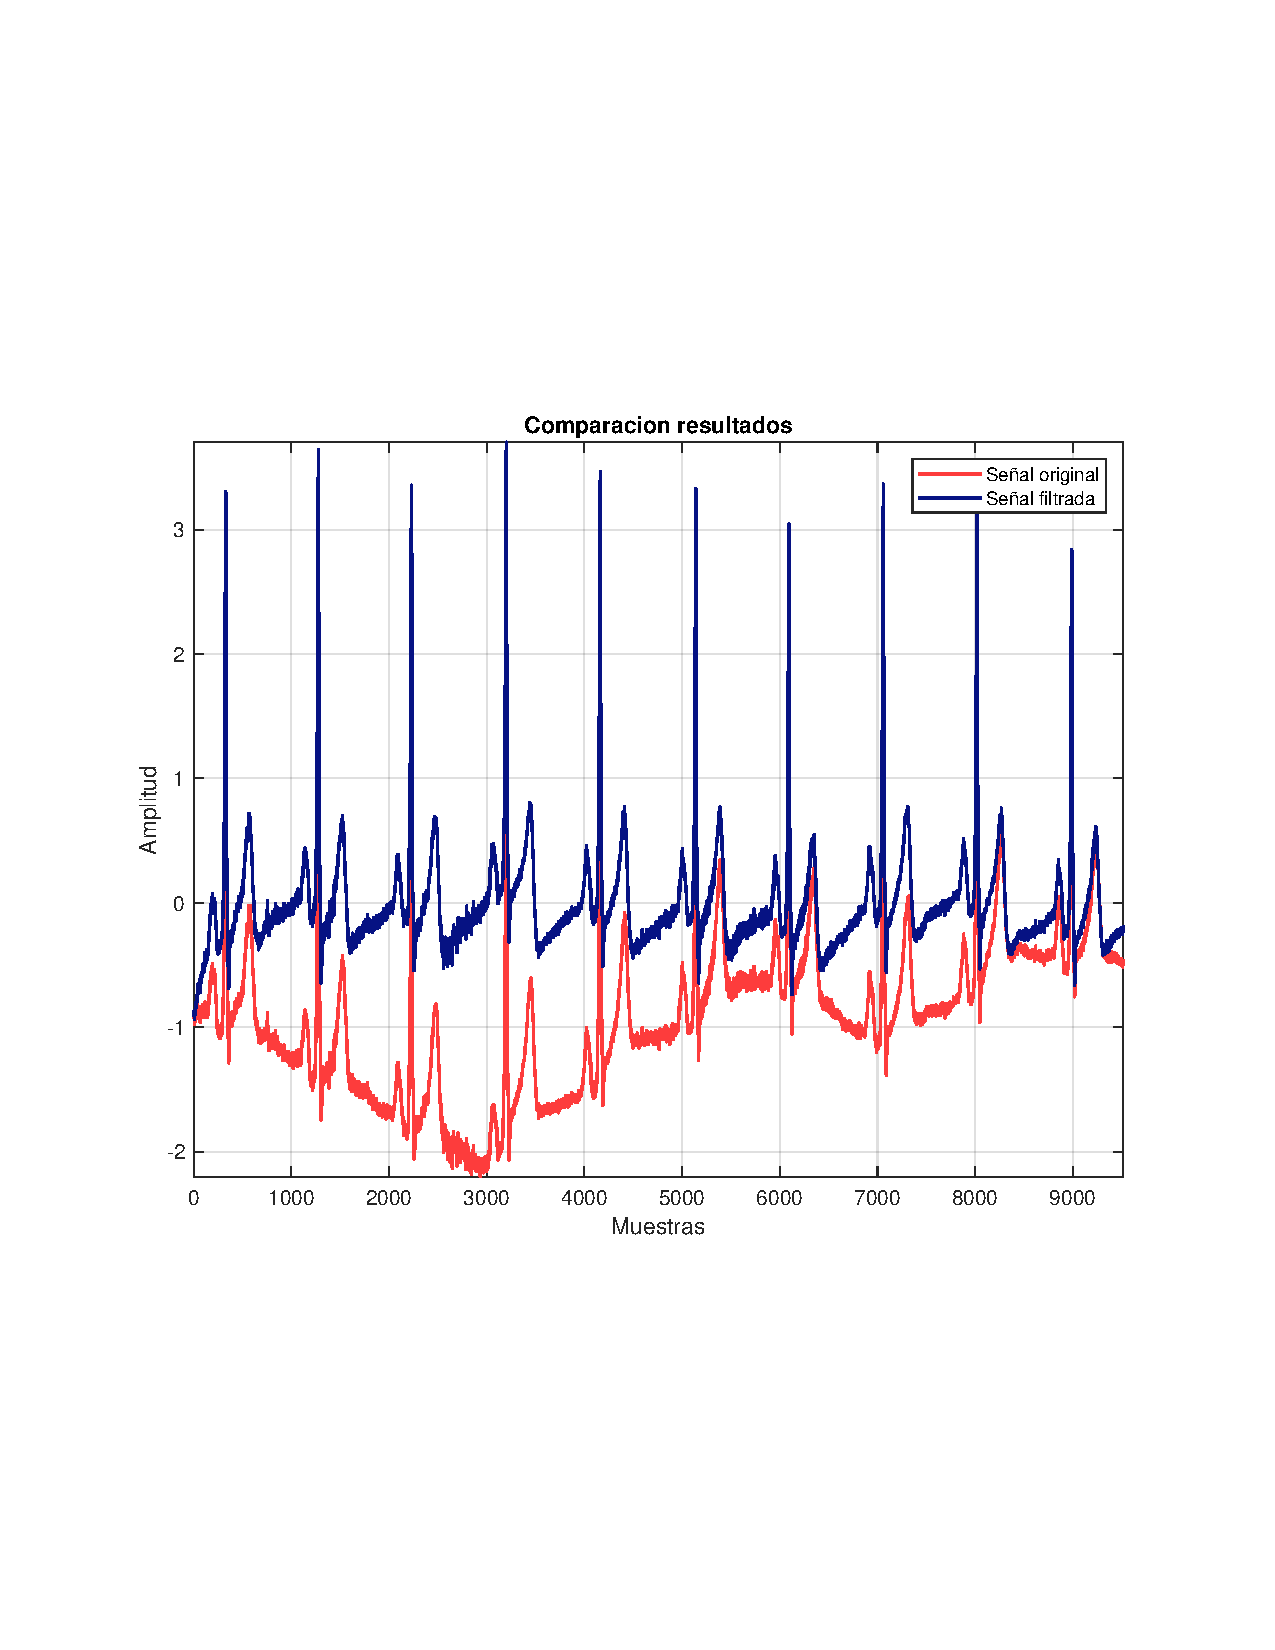
\includegraphics[width=0.6\textwidth,clip, trim = {1.9cm 6.8cm 2.3cm 7cm}]{../plots/1_c_ecg_filtered_2_freq_05.pdf}
			\caption{Resultado para filtro de orden n = 2, fc = 0.5}
			\label{fig:1_c_filter_n2_fc_05}
		\end{figure}
		
		\begin{figure}[H]
			\center
			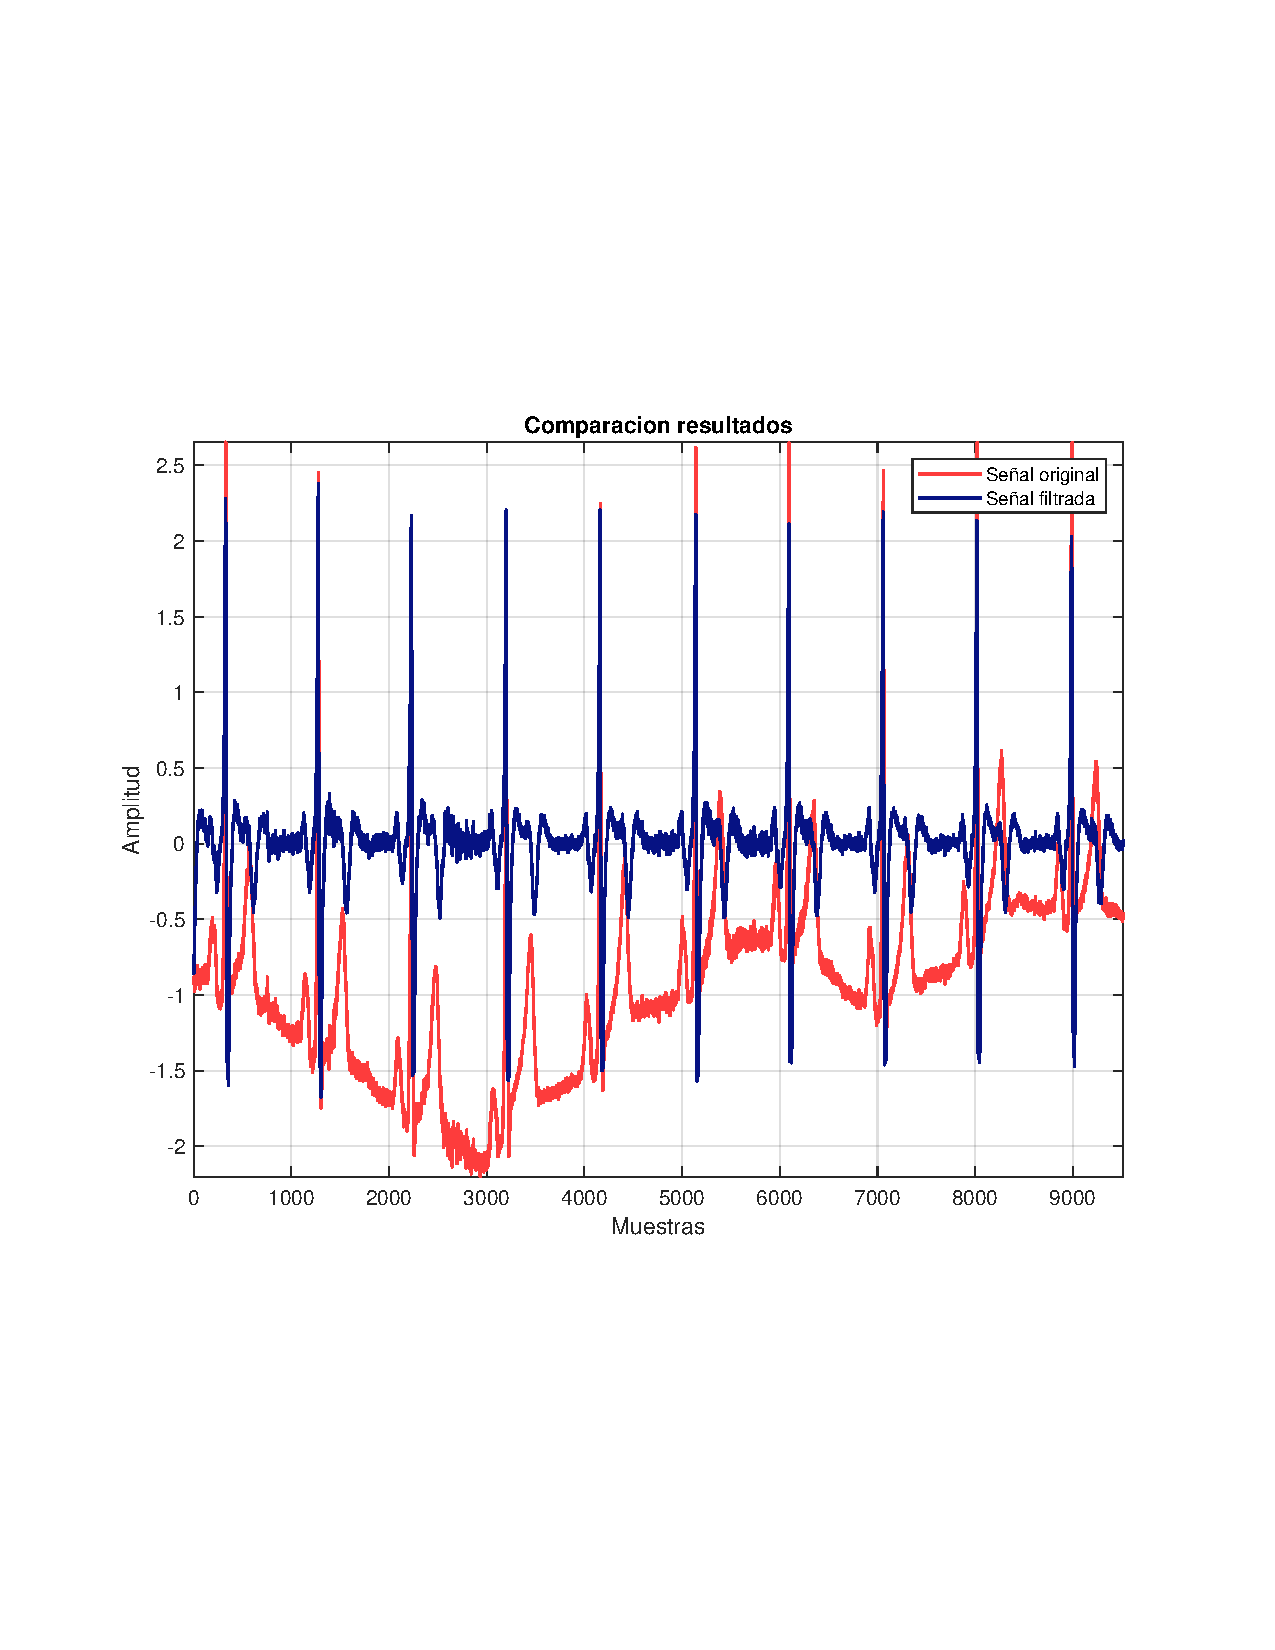
\includegraphics[width=0.6\textwidth,clip, trim = {1.9cm 6.8cm 2.3cm 7cm}]{../plots/1_c_ecg_filtered_2_freq_5.pdf}
			\caption{Resultado para filtro de orden n = 2, fc = 5}
			\label{fig:1_c_filter_n2_fc_5}
		\end{figure}
		
		\begin{figure}[H]
			\center
			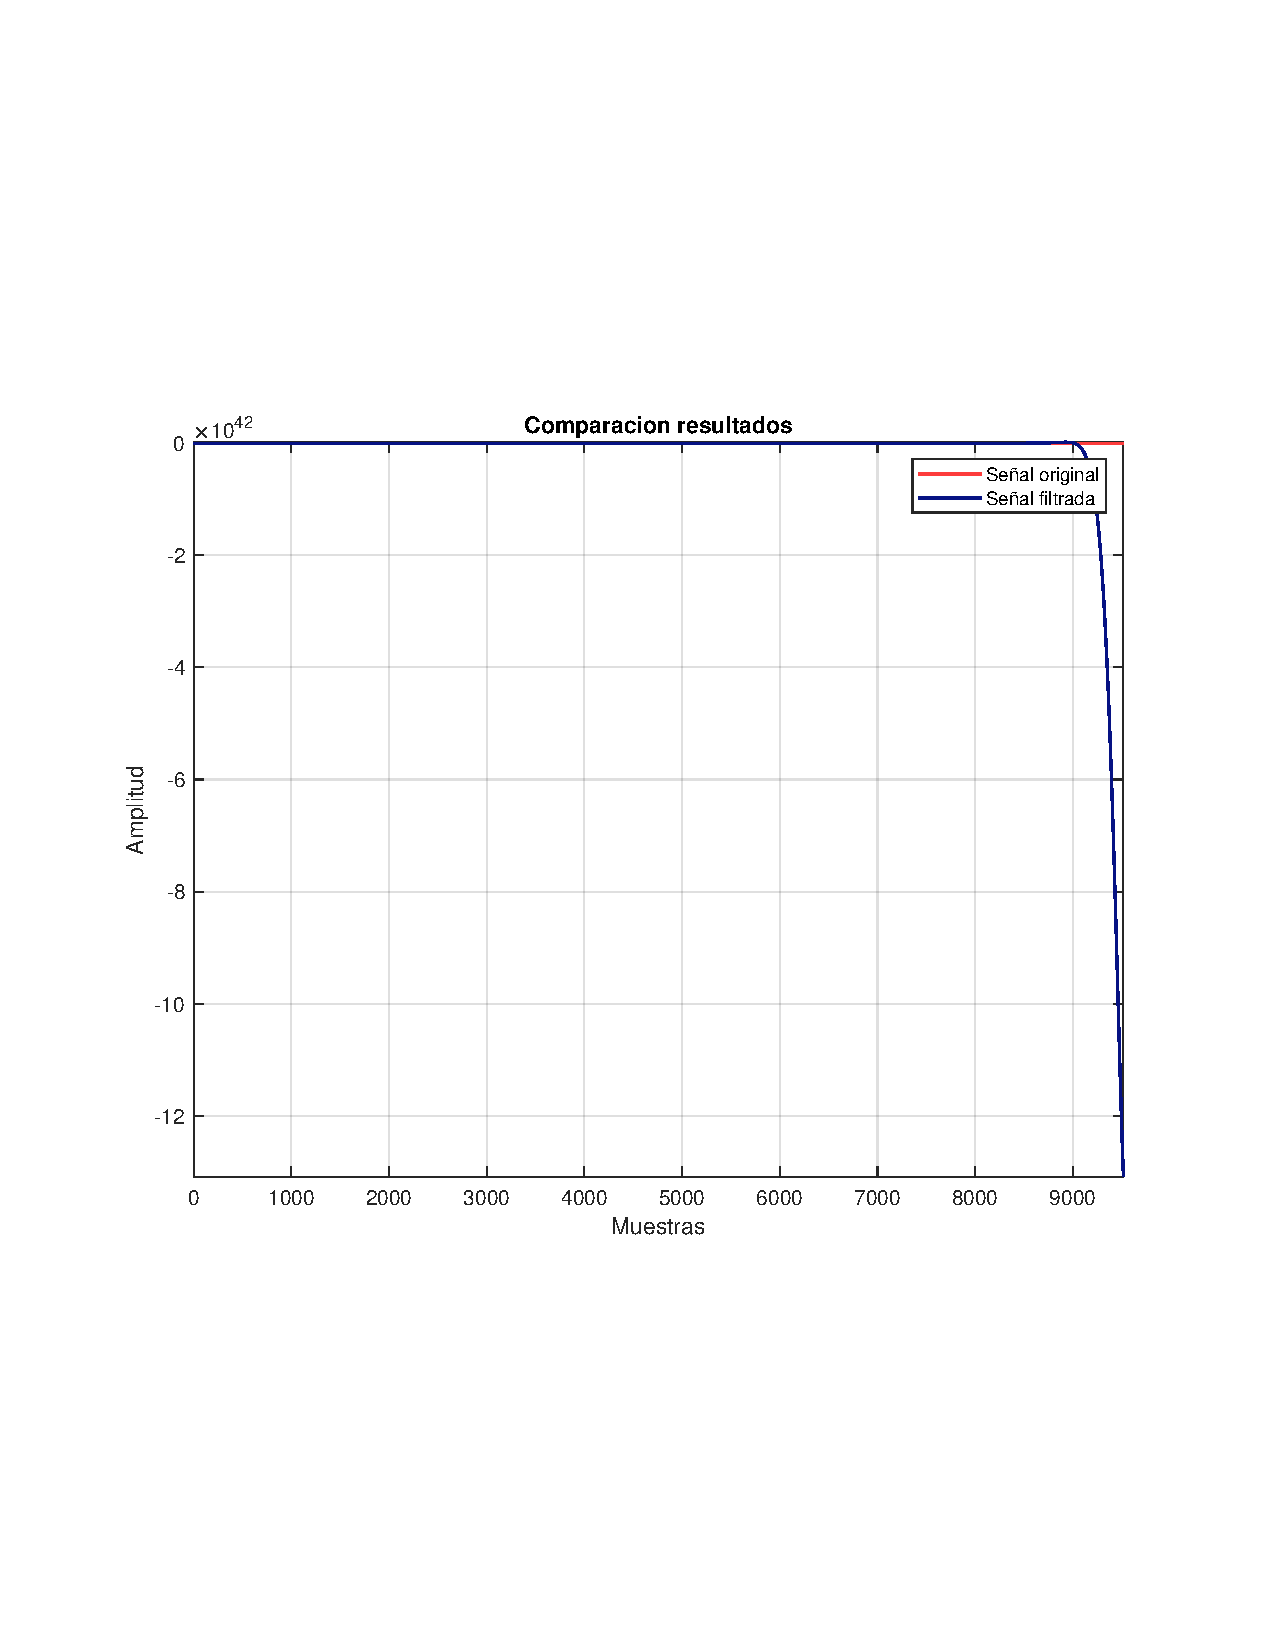
\includegraphics[width=0.6\textwidth,clip, trim = {1.9cm 6.8cm 2.3cm 7cm}]{../plots/1_c_ecg_filtered_8_freq_05.pdf}
			\caption{Resultado para filtro de orden n = 8, fc = 0.5}
			\label{fig:1_c_filter_n8_fc_05}
		\end{figure}
		
		\begin{figure}[H]
			\center
			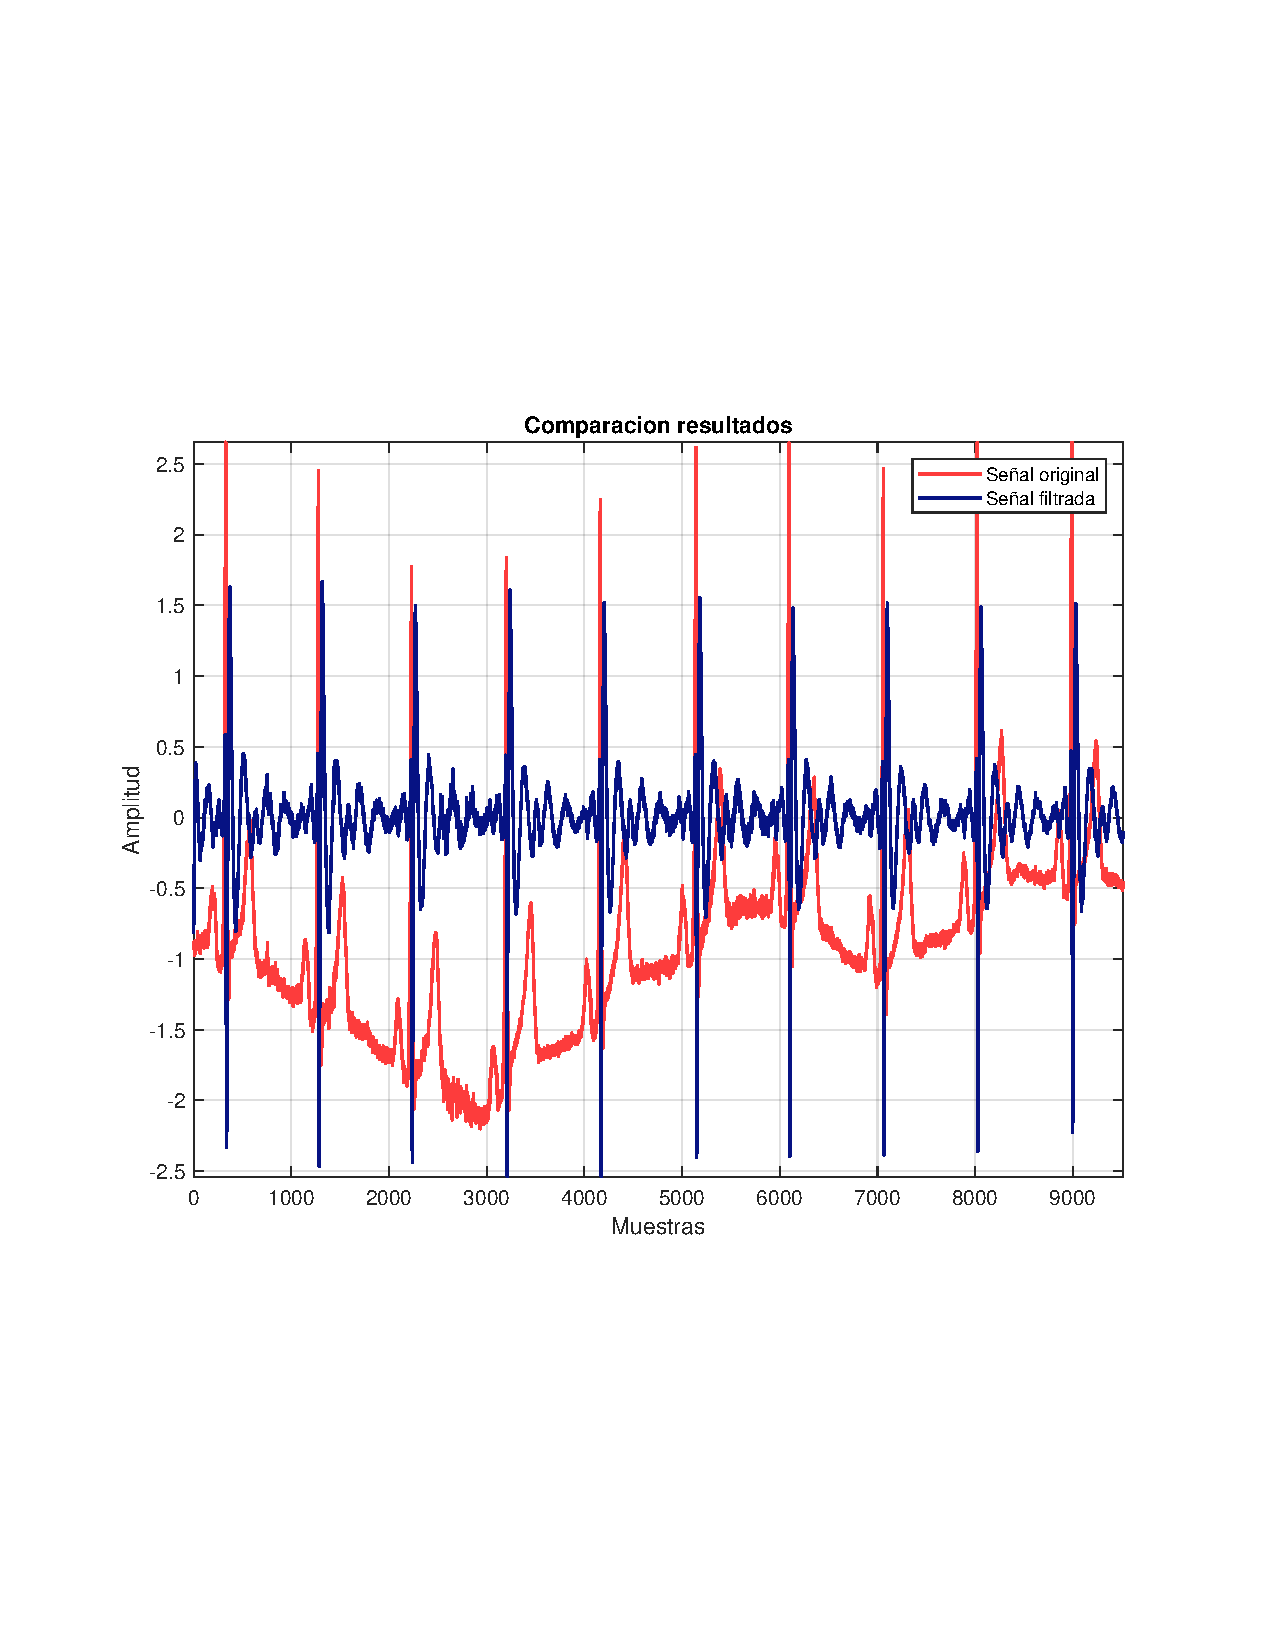
\includegraphics[width=0.6\textwidth,clip, trim = {1.9cm 6.8cm 2.3cm 7cm}]{../plots/1_c_ecg_filtered_8_freq_5.pdf}
			\caption{Resultado para filtro de orden n = 8, fc = 5}
			\label{fig:1_c_filter_n8_fc_5}
		\end{figure}
		
		A partir de estos resultados, se puede confirmar lo expuesto anteriormente el mejor resultado de filtrado, se obtiene para $n= 2$, y $fc = 0.5$, como se ve en la figura \ref{fig:1_c_filter_n2_fc_05}, dado que es el que mejor permite recuperar la señal sin causar distorsión evidente a la señal. Si bien el resultado obtenido en la figura \ref{fig:1_c_filter_n8_fc_5}, pareciera ser bueno, el segundo peak esperado para la señal ECG, se ve bastante atenuado en comparación a la señal original. Para el caso de la figura \ref{fig:1_c_filter_n2_fc_5}, se puede ver una evidente distorsión del segundo peak de la señal. Finalmente como se esperaba, para el filtro $n=8$ y $fc = 0.5$, hay completa destrucción de la señal, figura \ref{fig:1_c_filter_n8_fc_05}. Por lo que podemos concluir que para esta señal, lo más importante es preservar la fase de la señal original, y no tanto la atenuación de la banda DC, lo que concuerda con el filtro, de la figura \ref{fig:1_c_filter_n2_fc_05}. 
\newpage
\section{Identificación de vocales}
	\subsection{Análisis de DFT de las vocales}
	Calculando la \texttt{FFT} de las vocales, se procede a graficar la magnitud en \textit{dB}, para el intervalo $\left[ 0, 4000 \right]$~Hz. Se considera dos casos, uno donde la \texttt{FFT} se calcula con todos los valores de la señal y otro donde se calcula para el intervalo de muestras donde se encuentra la información de la vocal: 
	\begin{figure}[H]
		\center
		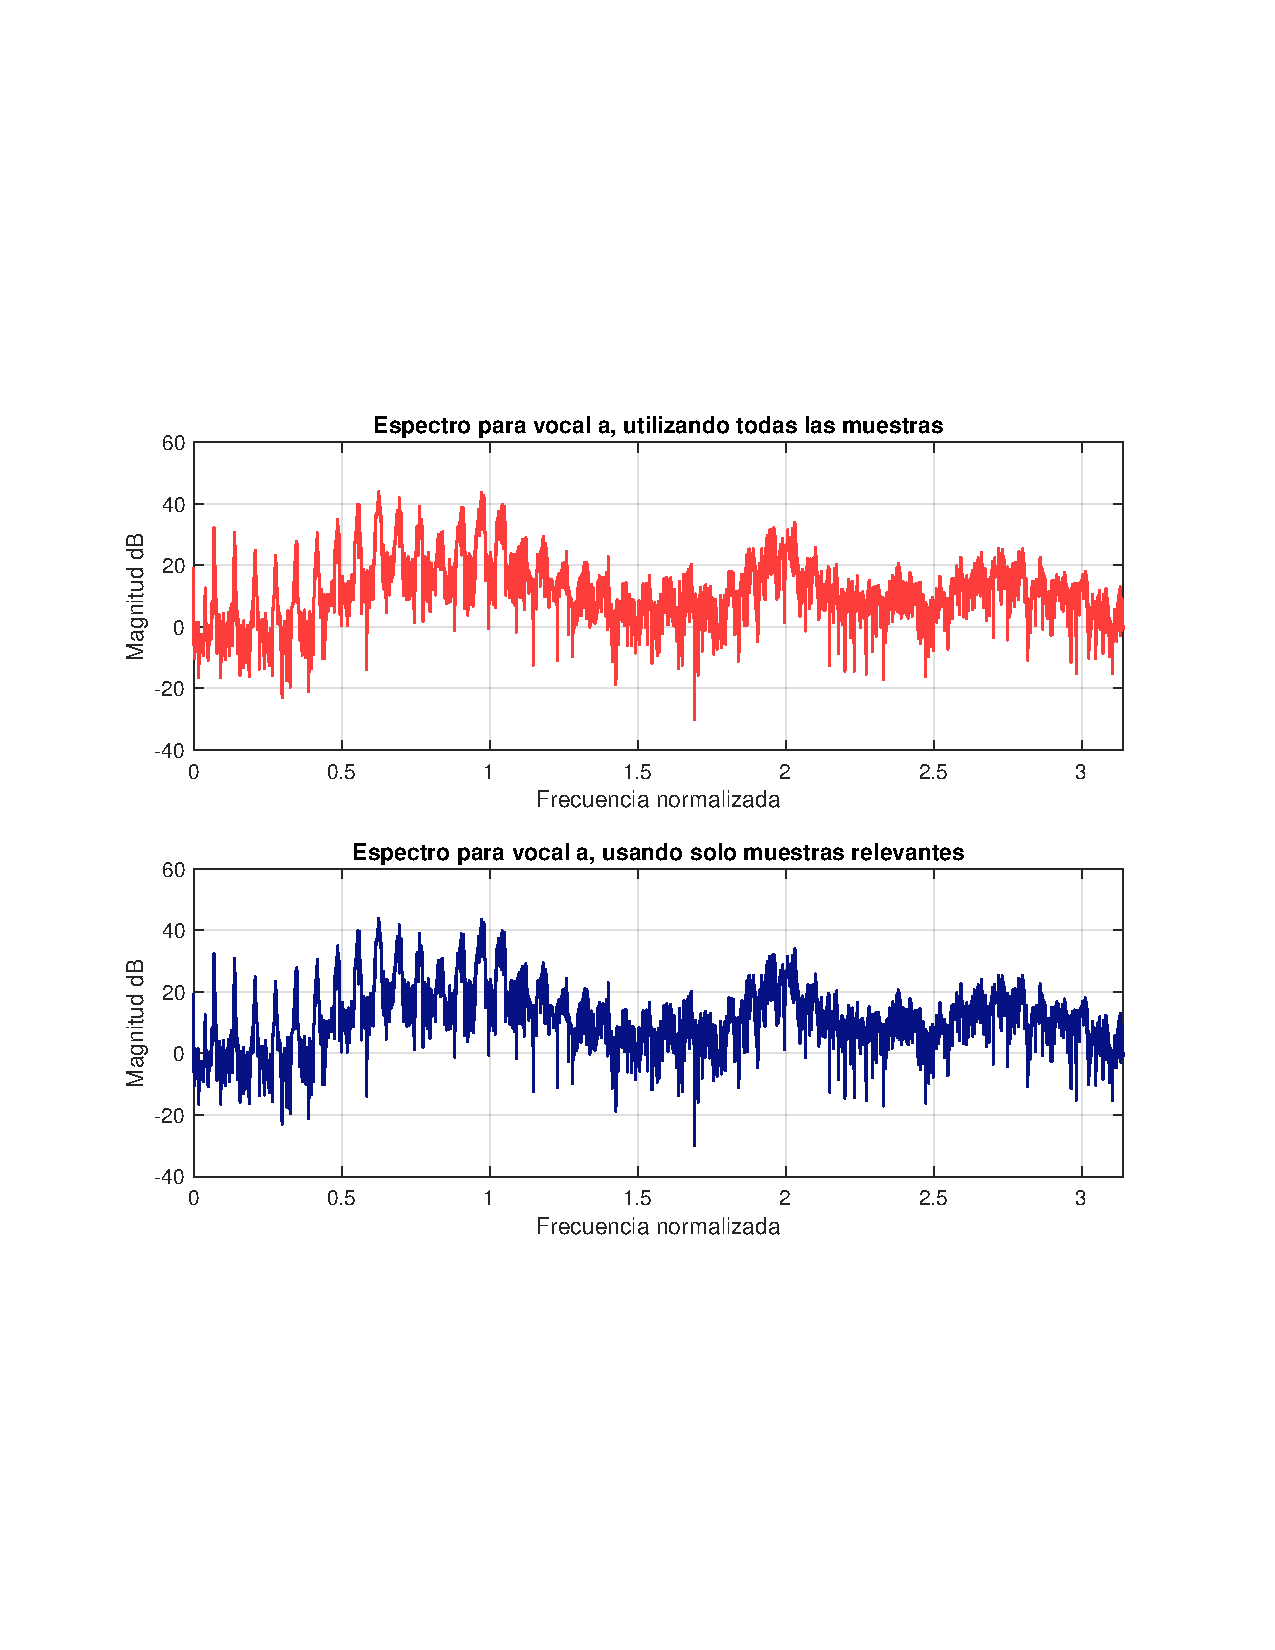
\includegraphics[width=0.6\textwidth,clip, trim = {1.9cm 6.8cm 2.3cm 7cm}]{../plots/a_fft.pdf}
		\caption{FFT para vocal a}
		\label{fig:a_fft}
	\end{figure}
	
	\begin{figure}[H]
		\center
		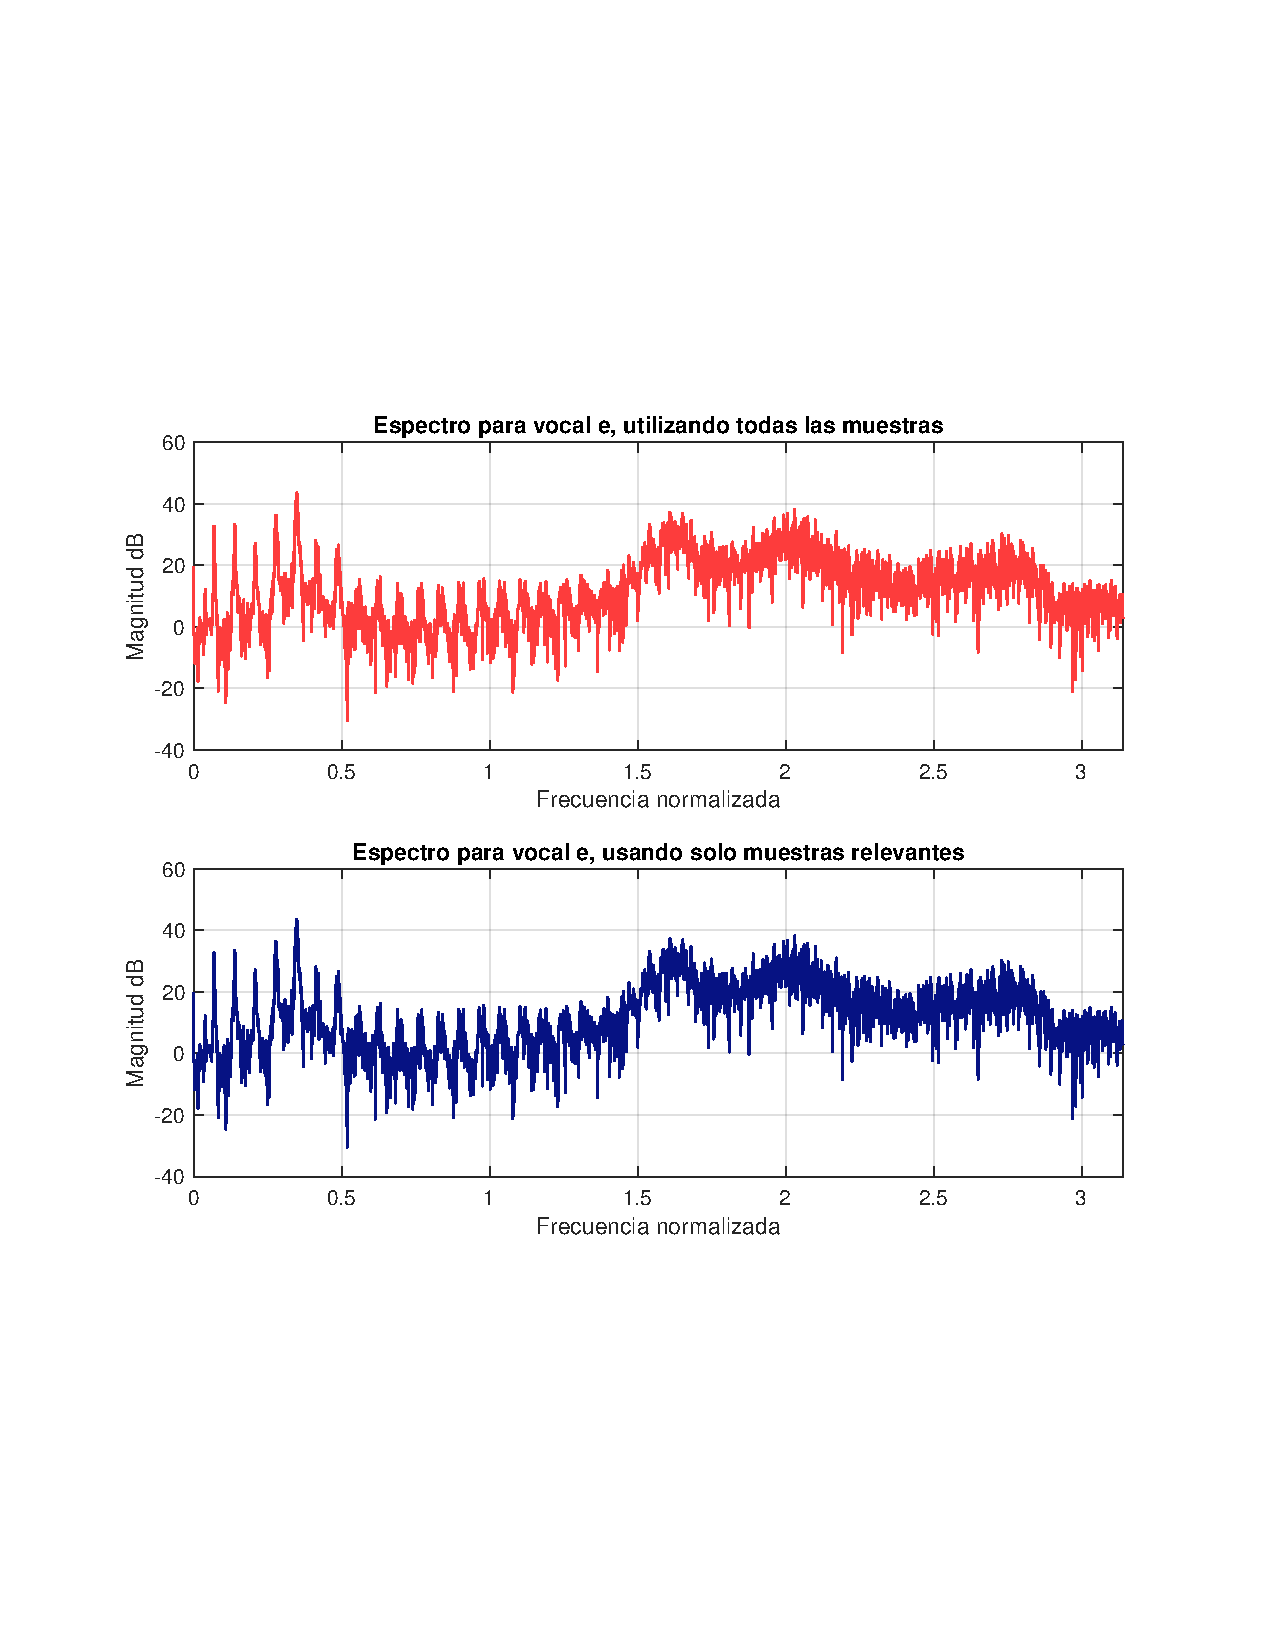
\includegraphics[width=0.6\textwidth,clip, trim = {1.9cm 6.8cm 2.3cm 7cm}]{../plots/e_fft.pdf}
		\caption{FFT para vocal e}
		\label{fig:e_fft}
	\end{figure}
	
	
	\begin{figure}[H]
		\center
		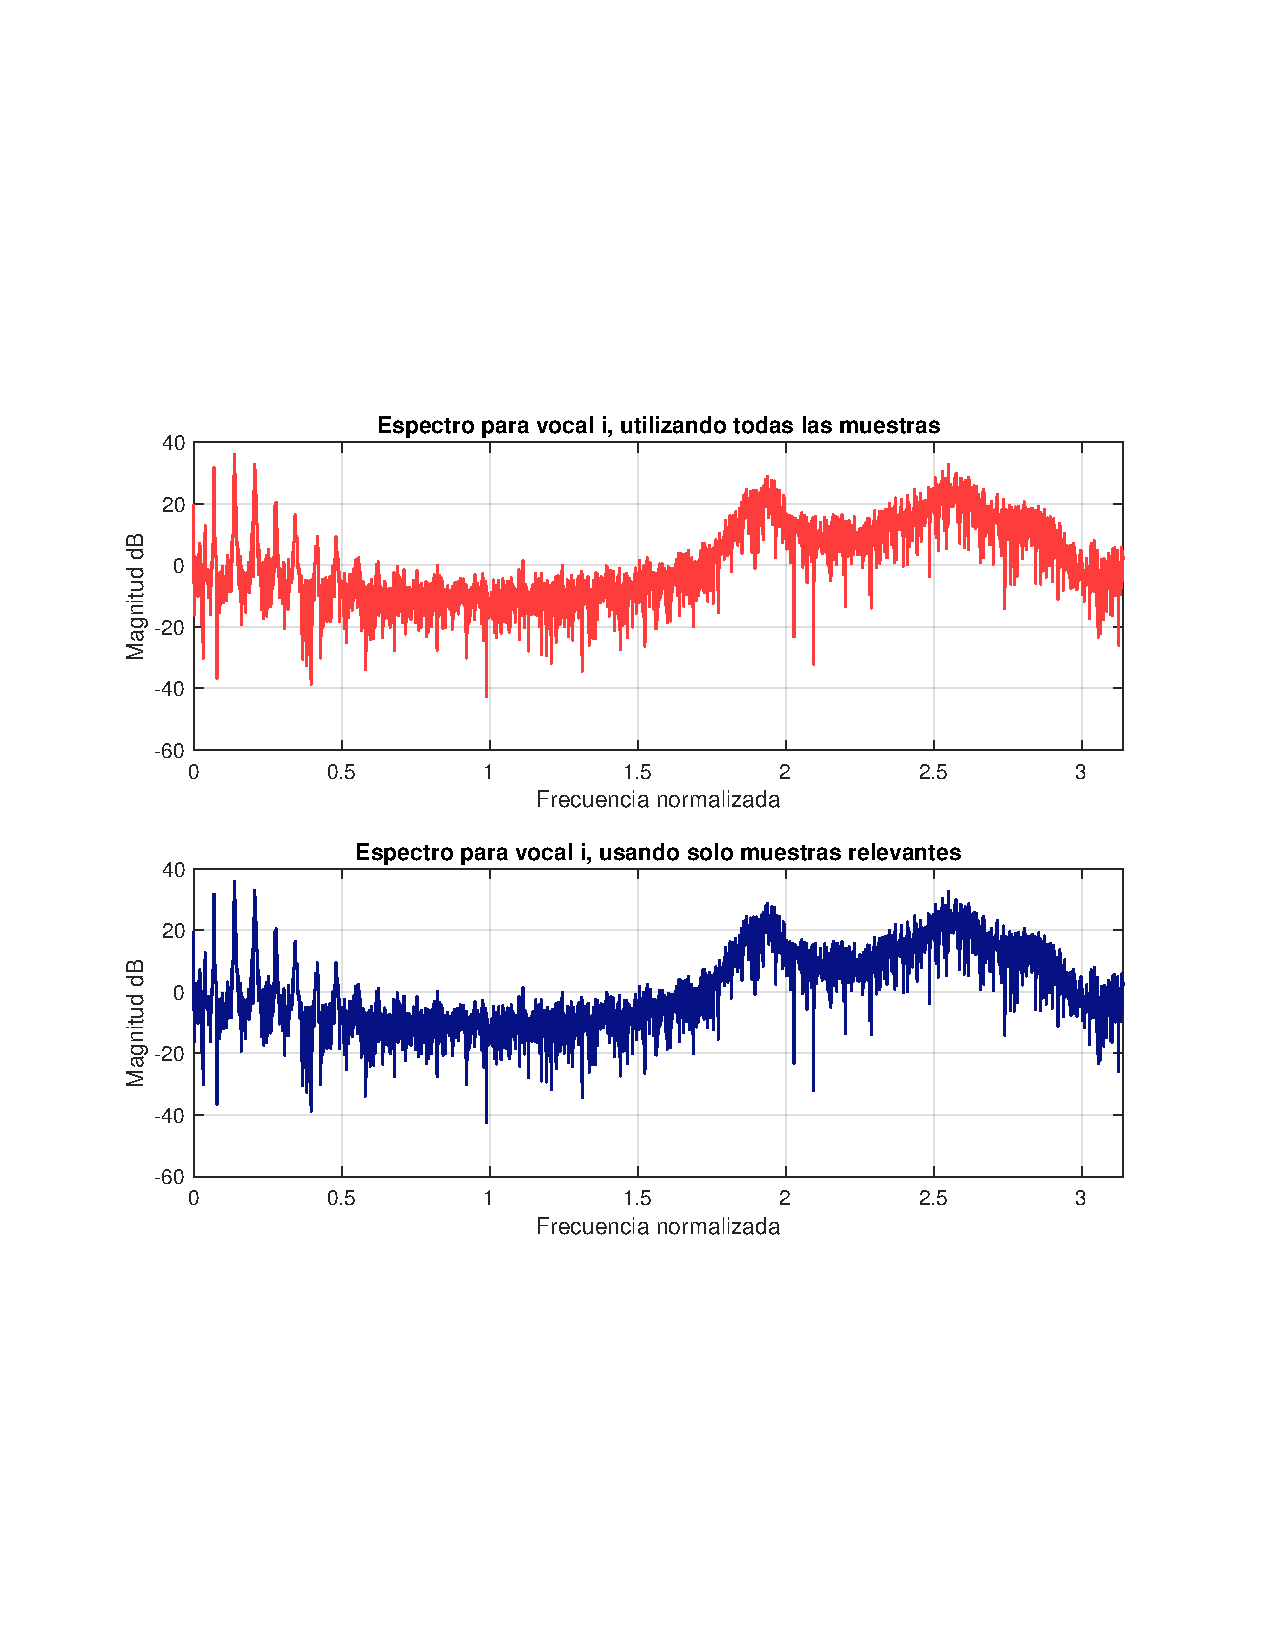
\includegraphics[width=0.6\textwidth,clip, trim = {1.9cm 6.8cm 2.3cm 7cm}]{../plots/i_fft.pdf}
		\caption{FFT para vocal i}
		\label{fig:i_fft}
	\end{figure}
	
	\begin{figure}[H]
		\center
		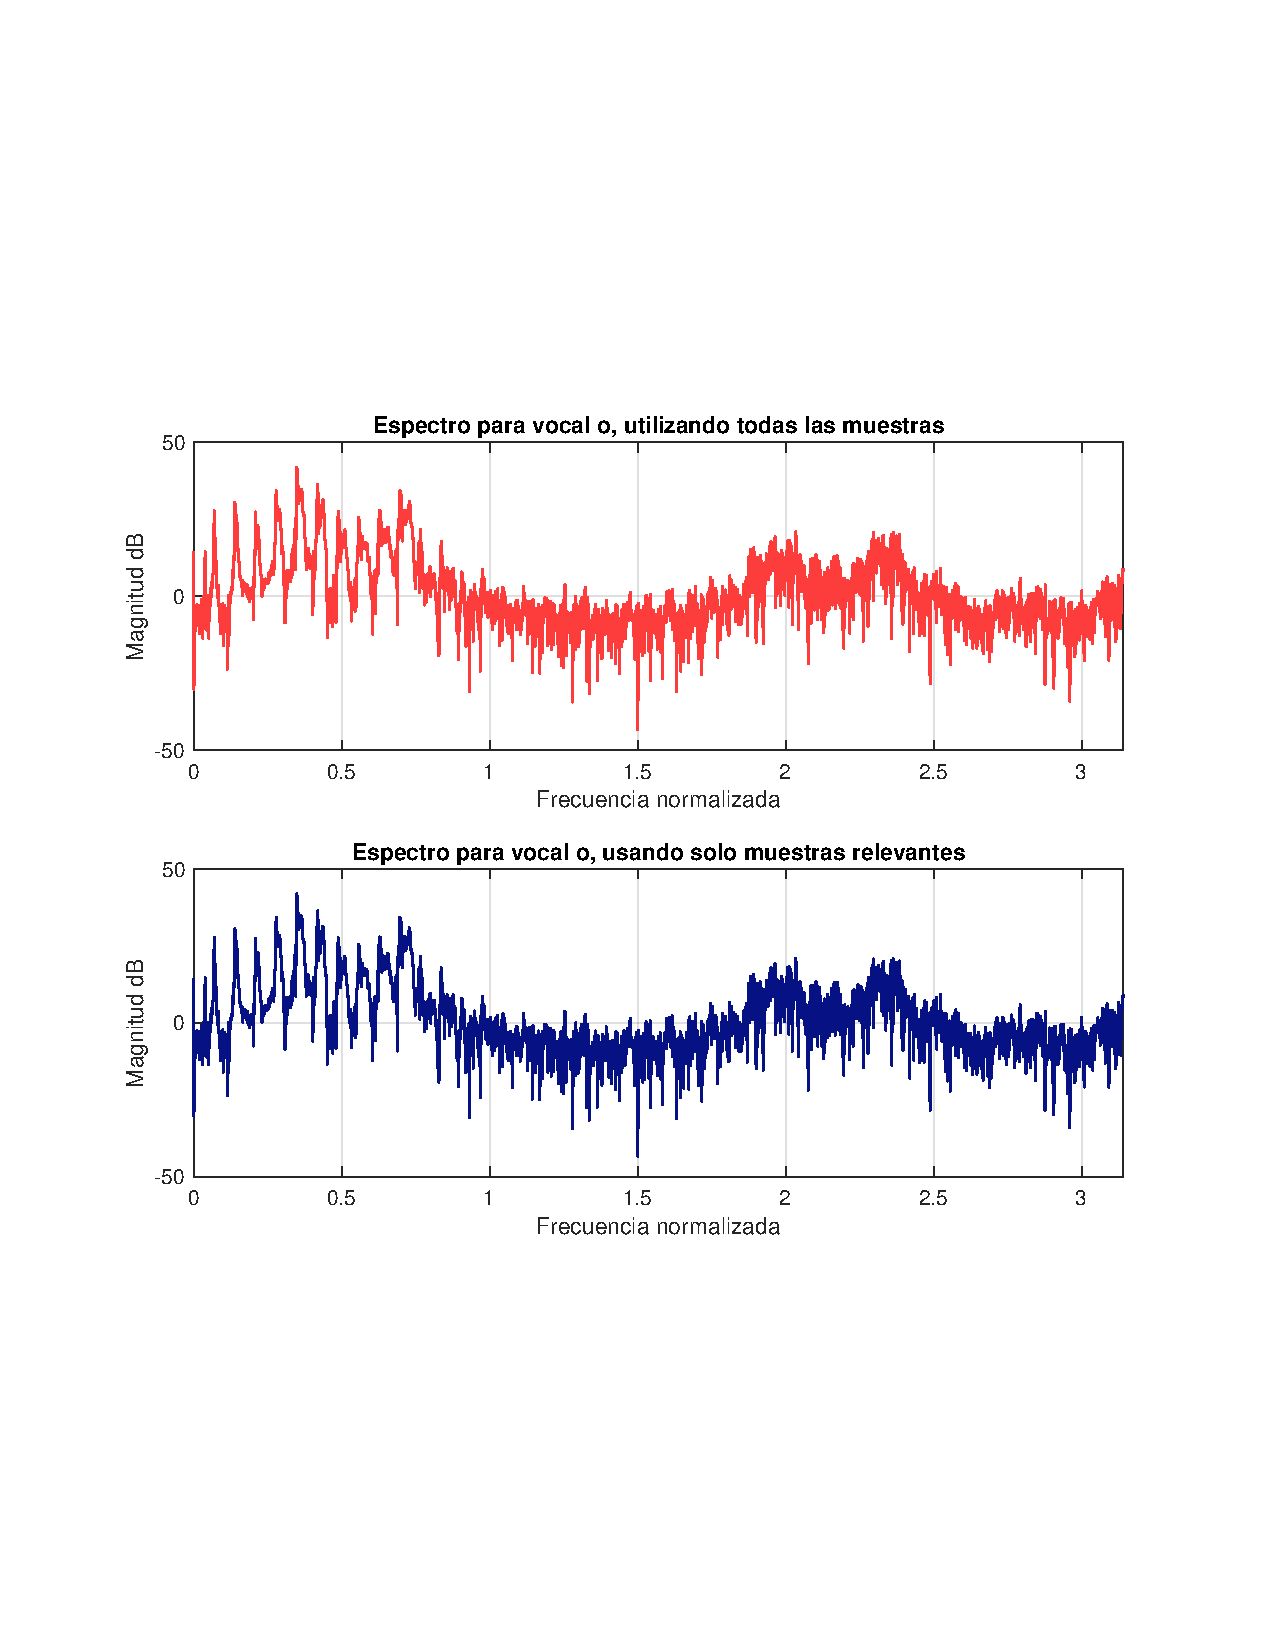
\includegraphics[width=0.6\textwidth,clip, trim = {1.9cm 6.8cm 2.3cm 7cm}]{../plots/o_fft.pdf}
		\caption{FFT para vocal o}
		\label{fig:o_fft}
	\end{figure}
	
	\begin{figure}[H]
		\center
		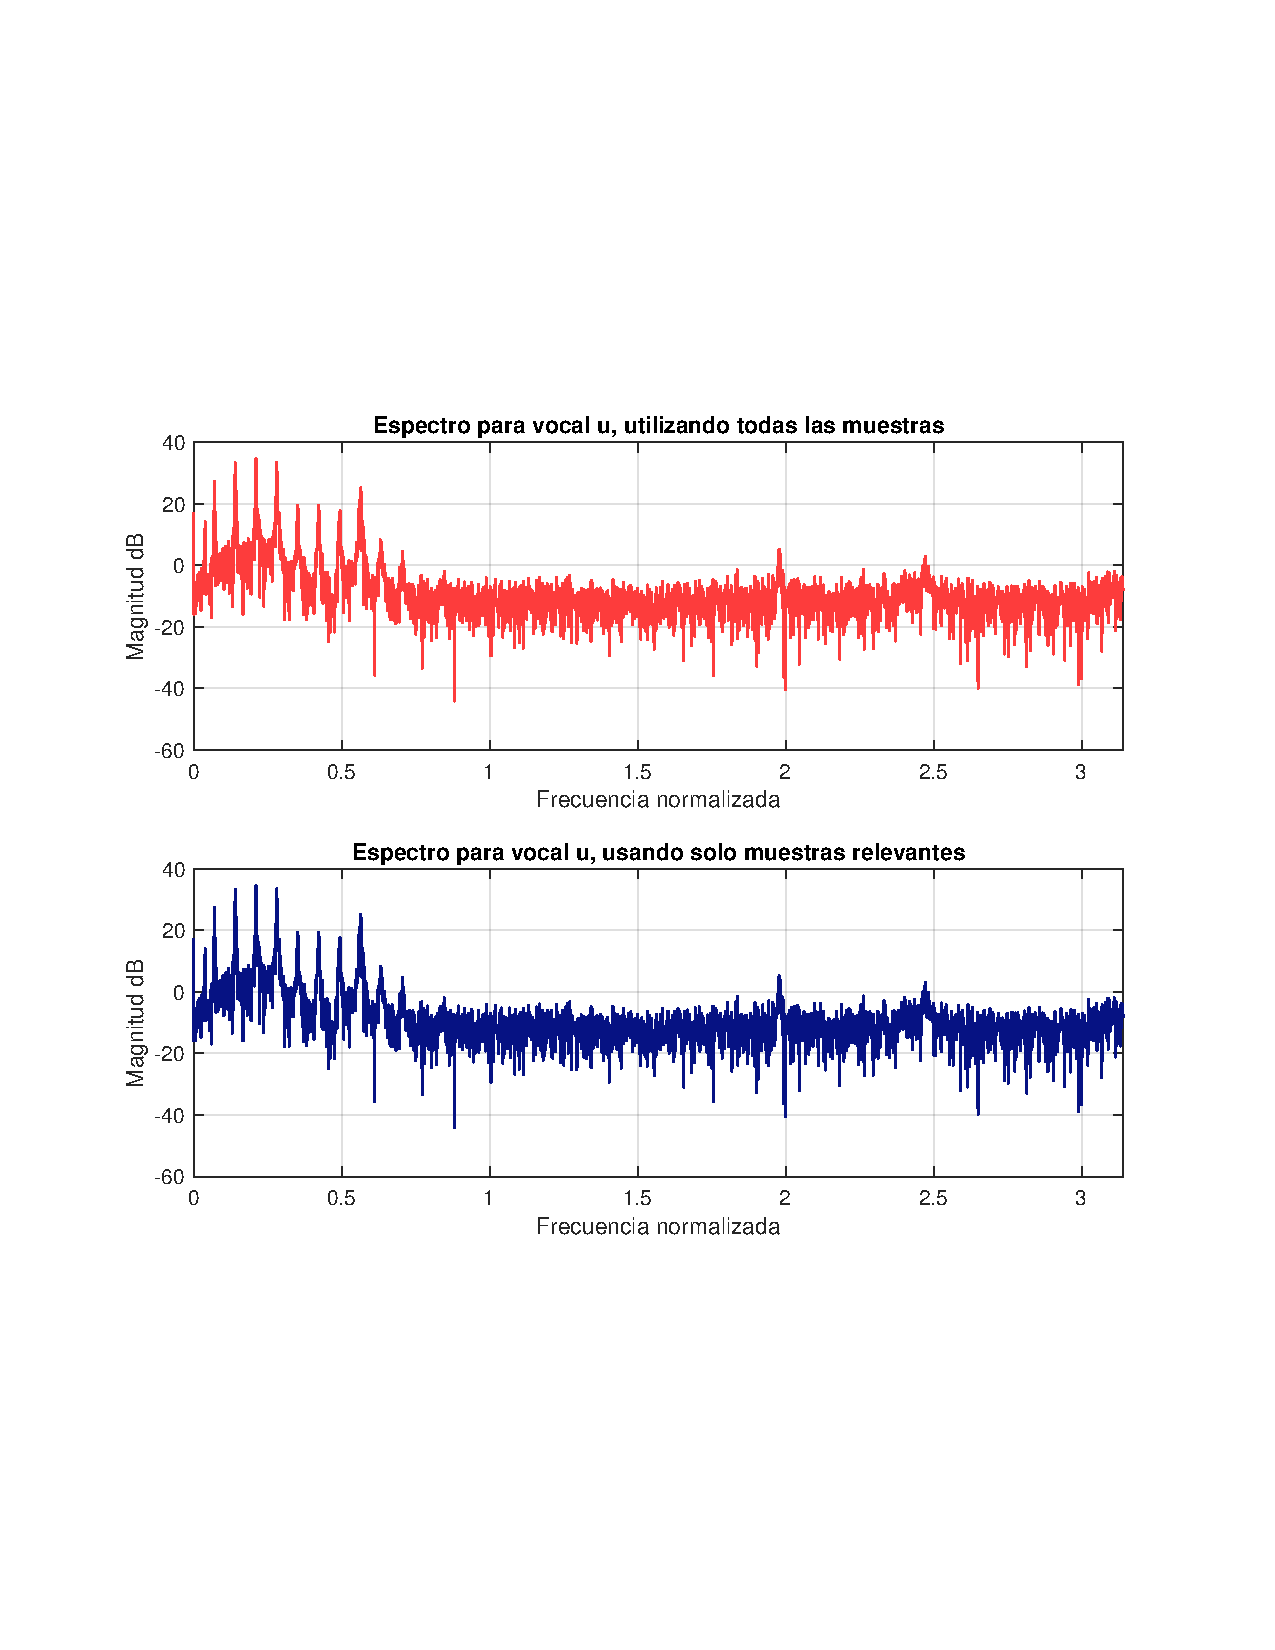
\includegraphics[width=0.6\textwidth,clip, trim = {1.9cm 6.8cm 2.3cm 7cm}]{../plots/u_fft.pdf}
		\caption{FFT para vocal u}
		\label{fig:u_fft}
	\end{figure}
	
	
	Analizando los resultados, se puede ver que, de manera visual, los espectros donde se consideró únicamente la porción que contenía información de la señal, se ve menos saturado, que para los que se consideró la señal completa. Esto se puede explicar, principalmente debido a que para las secciones donde la información de la vocal no se encuentra presente, no se tiene una situación de tipo \textit{zero-padding}, sino que se tiene ruido asociado al equipo de grabación. Por lo que al seleccionar únicamente la información de la señal, estamos limitando el ruido que se introduce al espectro. Es por esto, que se recomienda trabajar con la porción con información, dejando fuera los instantes donde solo hay \textit{ruido de background}.
	
	\subsection{Análisis de formantes}
	
	A partir de los gráficos obtenidos en el punto anterior, se procede a obtener la frecuencia fundamental de las vocales, además de sus primeras dos formantes, los resultados se entregan en la siguiente tabla:
	
	\begin{table}[H]
		\center
		\begin{tabular}{|c|c|c|c|}
			\hline
			\textbf{Vocal} & \textbf{Fundamental Hz} & \textbf{F1 Hz} & \textbf{F2 Hz} \\
			\hline 
			A & 87 & 796 & 1239 \\
			\hline
			E & 87 & 444 & 2037 \\
			\hline
			I & 87 & 175 & 2468 \\
			\hline
			O & 89 & 444 & 886 \\
			\hline
			U & 89 & 267 & 719 \\
			\hline
		\end{tabular}
		\caption{Tabla de frecuencia fundamental y formantes, para las distintas vocales}
		\label{tab:formantes-freq}
	\end{table}
	
	Graficando F1 v/s F2, para generar el triángulo vocálico:

	\begin{figure}[H]
		\center
		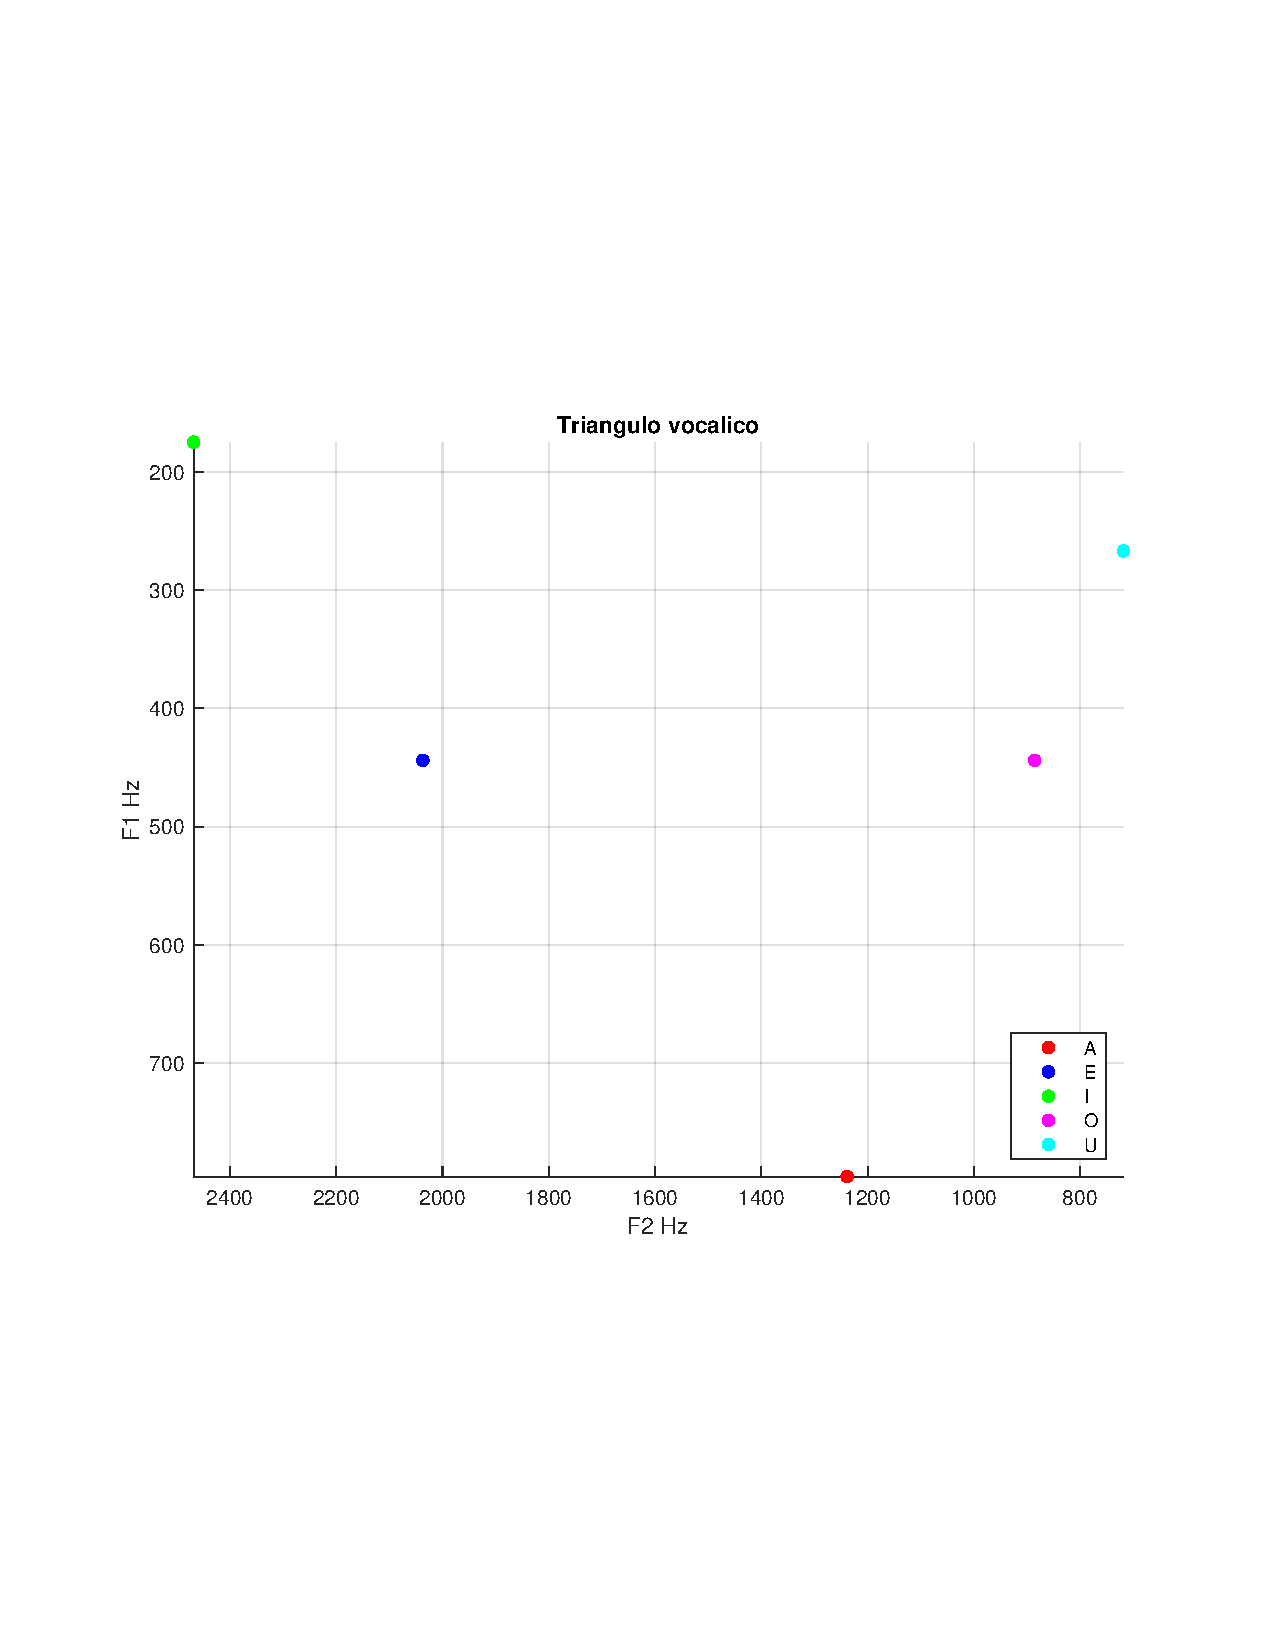
\includegraphics[width=0.6\textwidth,clip, trim = {1.9cm 6.8cm 2.3cm 7cm}]{../plots/vocalic_triang.pdf}
		\caption{Triángulo vocálico obtenido}
		\label{fig:vocal_triang}
	\end{figure}
	
	Note que para generarlo, se tiene que invertir la dirección de los ejes, dado que se define el origen en la esquina superior derecha. Comparando este resultado con el esperado de forma teórica, se puede ver que se comporta de manera similar:
	\begin{figure}[H]
		\center
		
\includegraphics[width = 0.6\linewidth]{../plots/1280px-Spanish_vowel_chart.png}
		\caption{Triángulo vocálico teórico. Cortesía de Wikipedia}
		\label{fig:triang_vocal_teorico}
	\end{figure}
	
	
	\subsection{LPC}
		Utilizando la función \texttt{lpc(x,p)} de \textsc{Matlab} se procede a obtener los filtros IIR asociados a cada vocal. Graficando la magnitud de su respuesta en frecuencia y comparando con el espectro de la vocal se obtiene:
		
	
	\begin{figure}[H]
		\center
		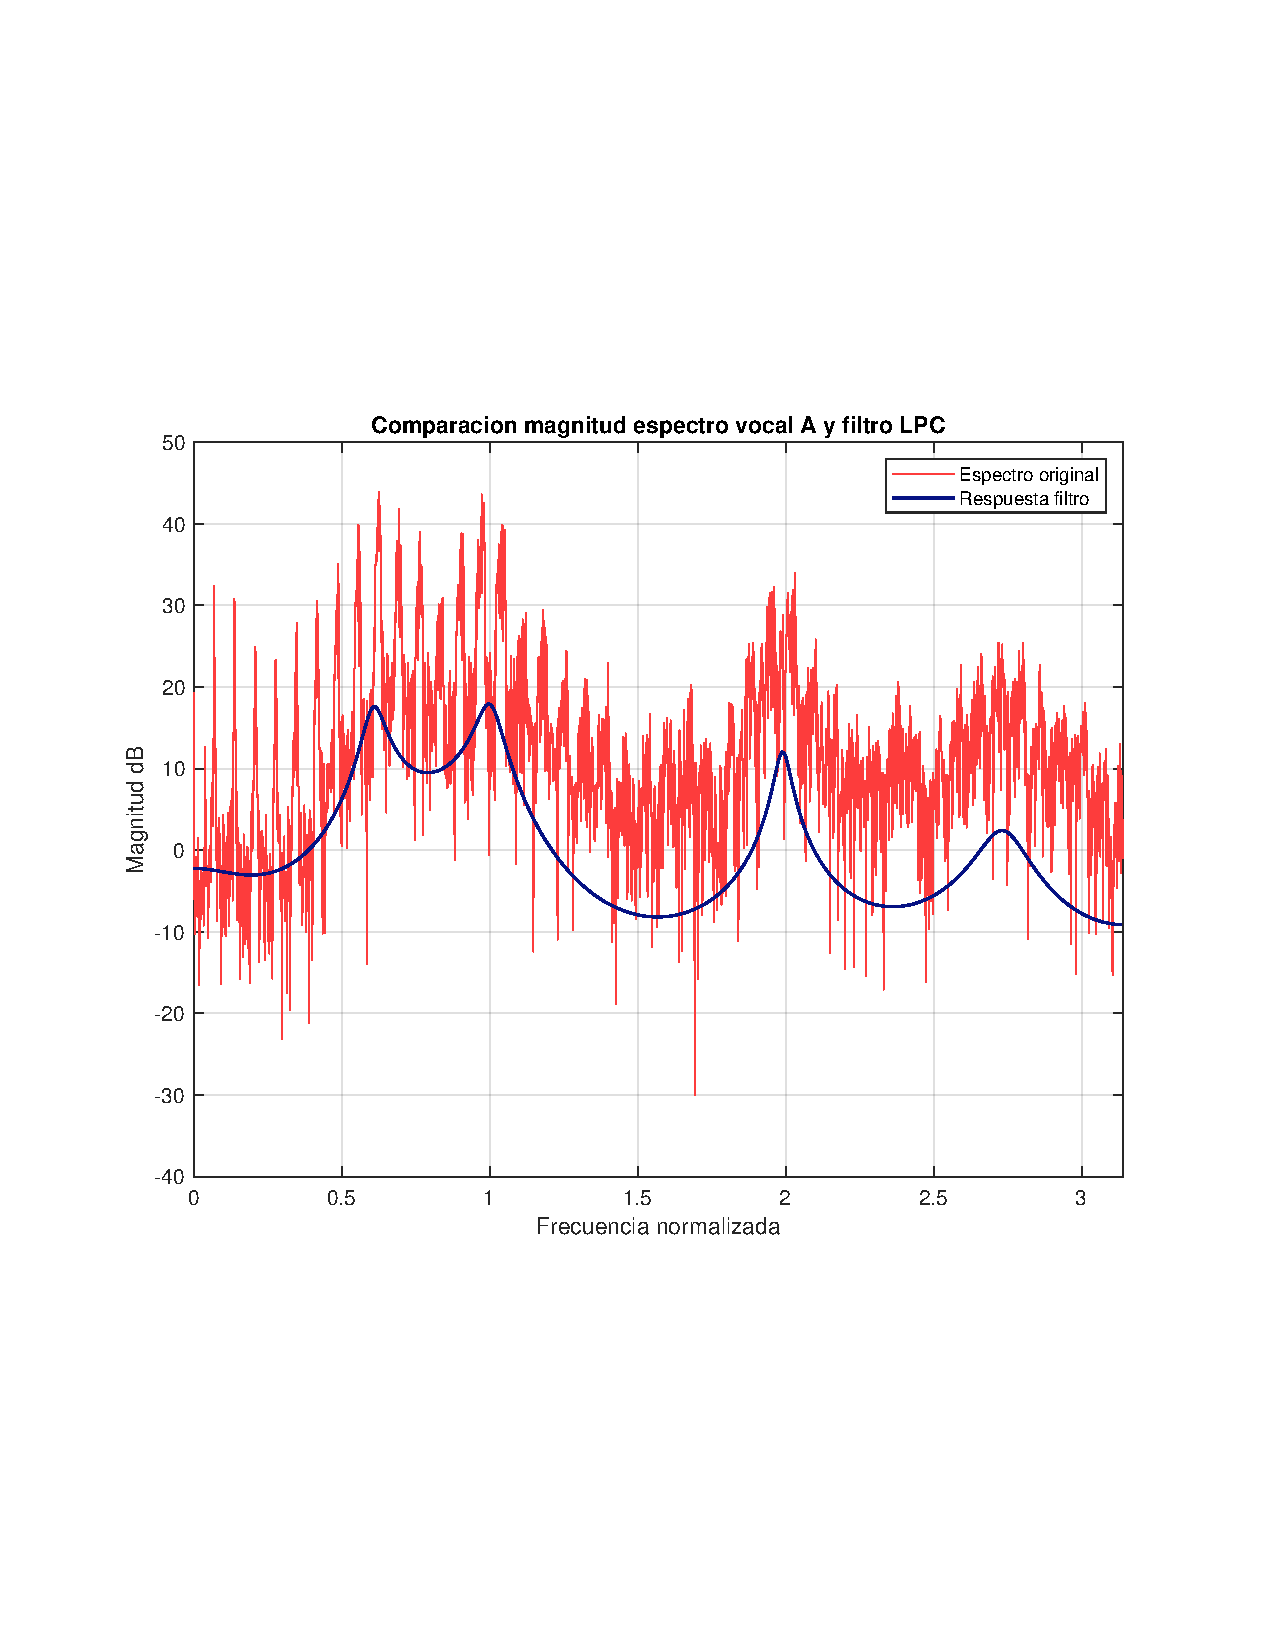
\includegraphics[width=0.6\textwidth,clip, trim = {1.9cm 6.8cm 2.3cm 7cm}]{../plots/A_lpc.pdf}
		\caption{Comparación espectro y filtro LPC: A}
		\label{fig:LPC_A}
	\end{figure}

	\begin{figure}[H]
		\center
		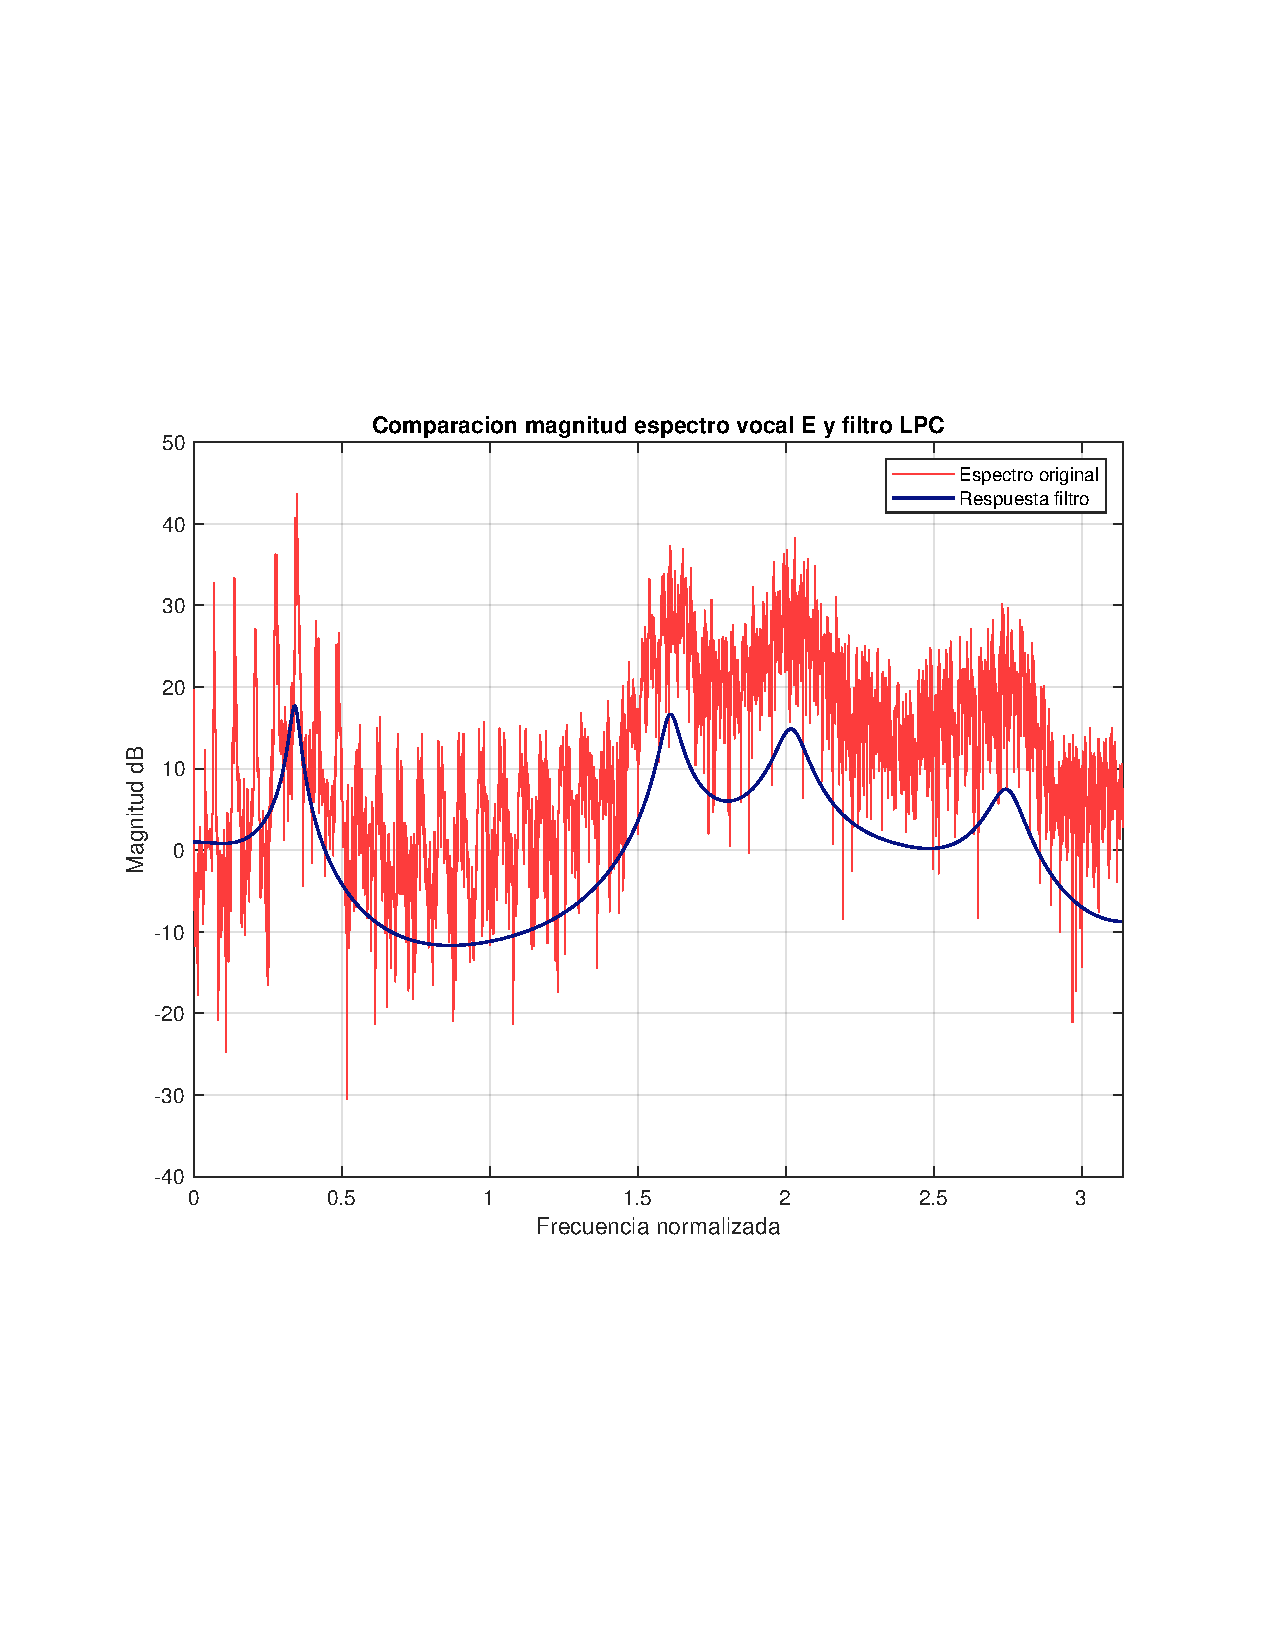
\includegraphics[width=0.6\textwidth,clip, trim = {1.9cm 6.8cm 2.3cm 7cm}]{../plots/E_lpc.pdf}
		\caption{Comparación espectro y filtro LPC: E}
		\label{fig:LPC_E}
	\end{figure}

	\begin{figure}[H]
		\center
		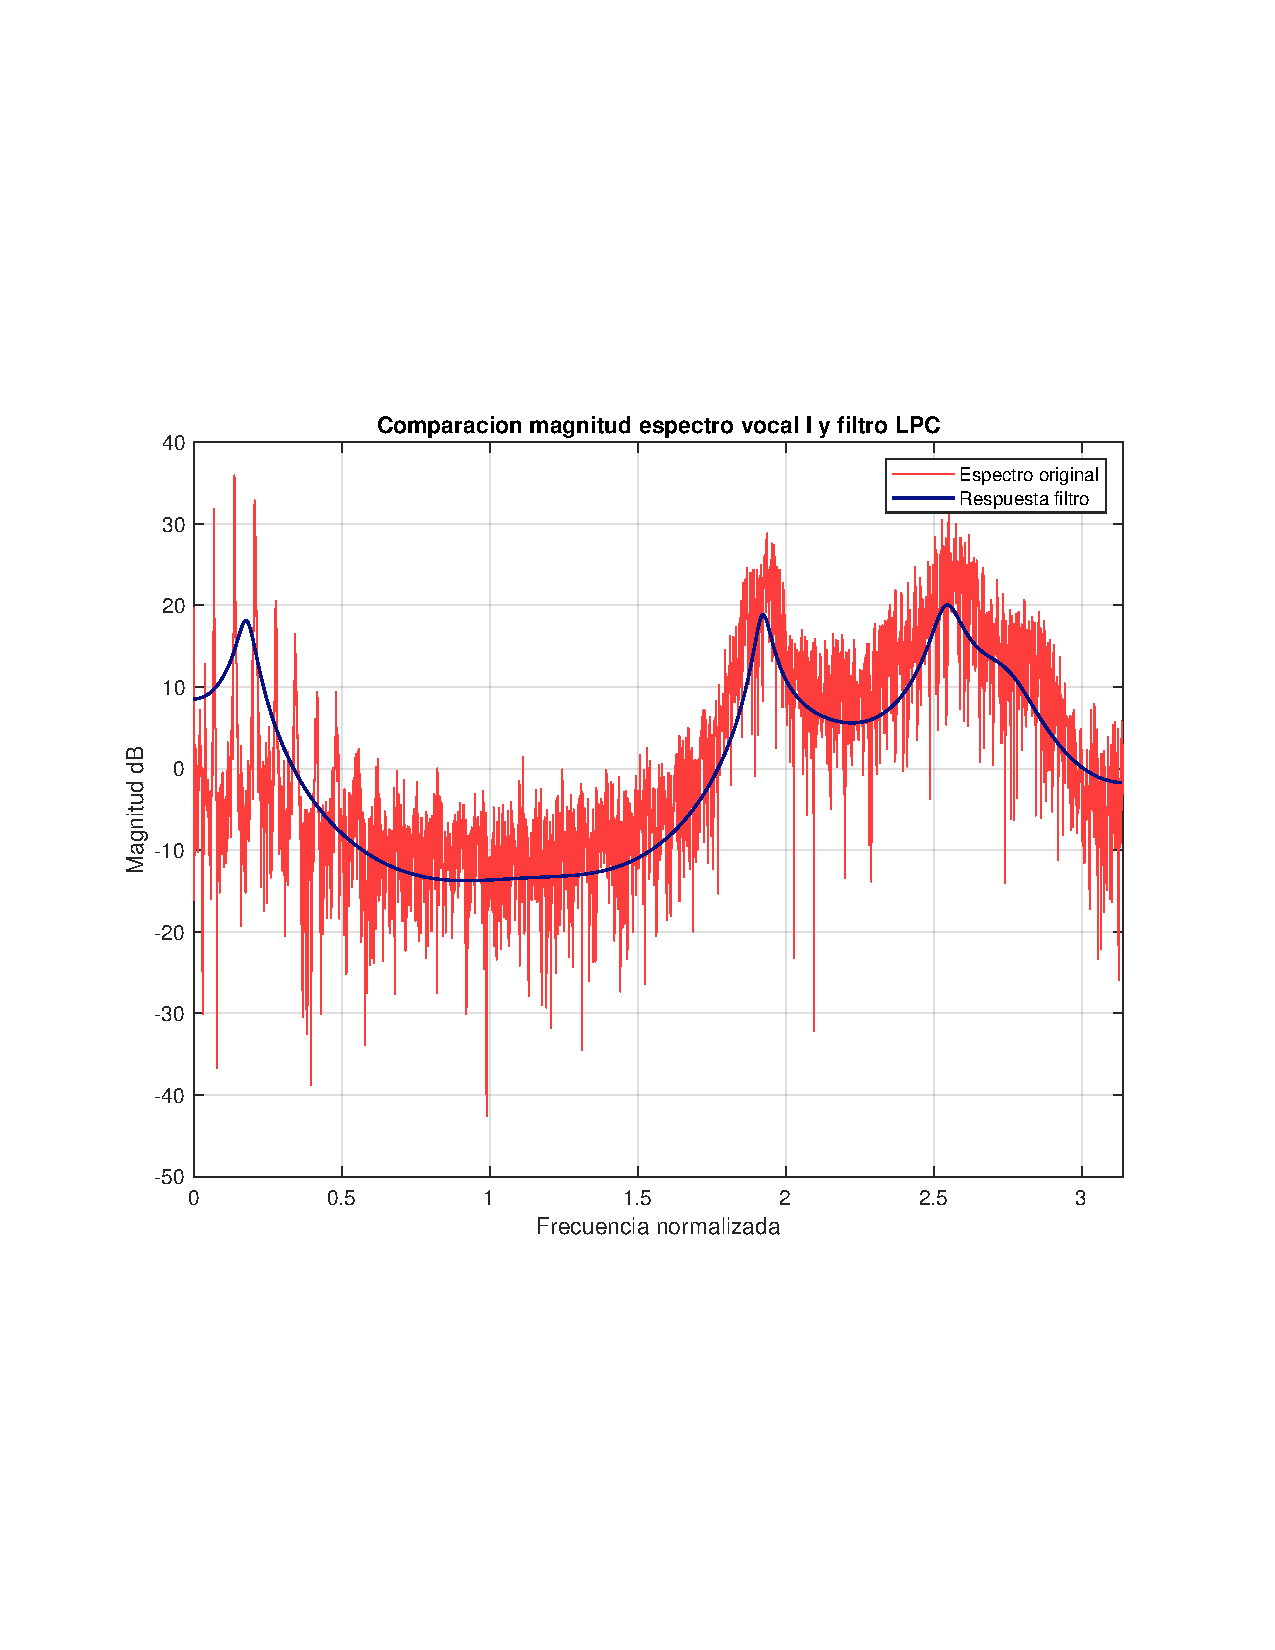
\includegraphics[width=0.6\textwidth,clip, trim = {1.9cm 6.8cm 2.3cm 7cm}]{../plots/I_lpc.pdf}
		\caption{Comparación espectro y filtro LPC: I}
		\label{fig:LPC_I}
	\end{figure}

	\begin{figure}[H]
		\center
		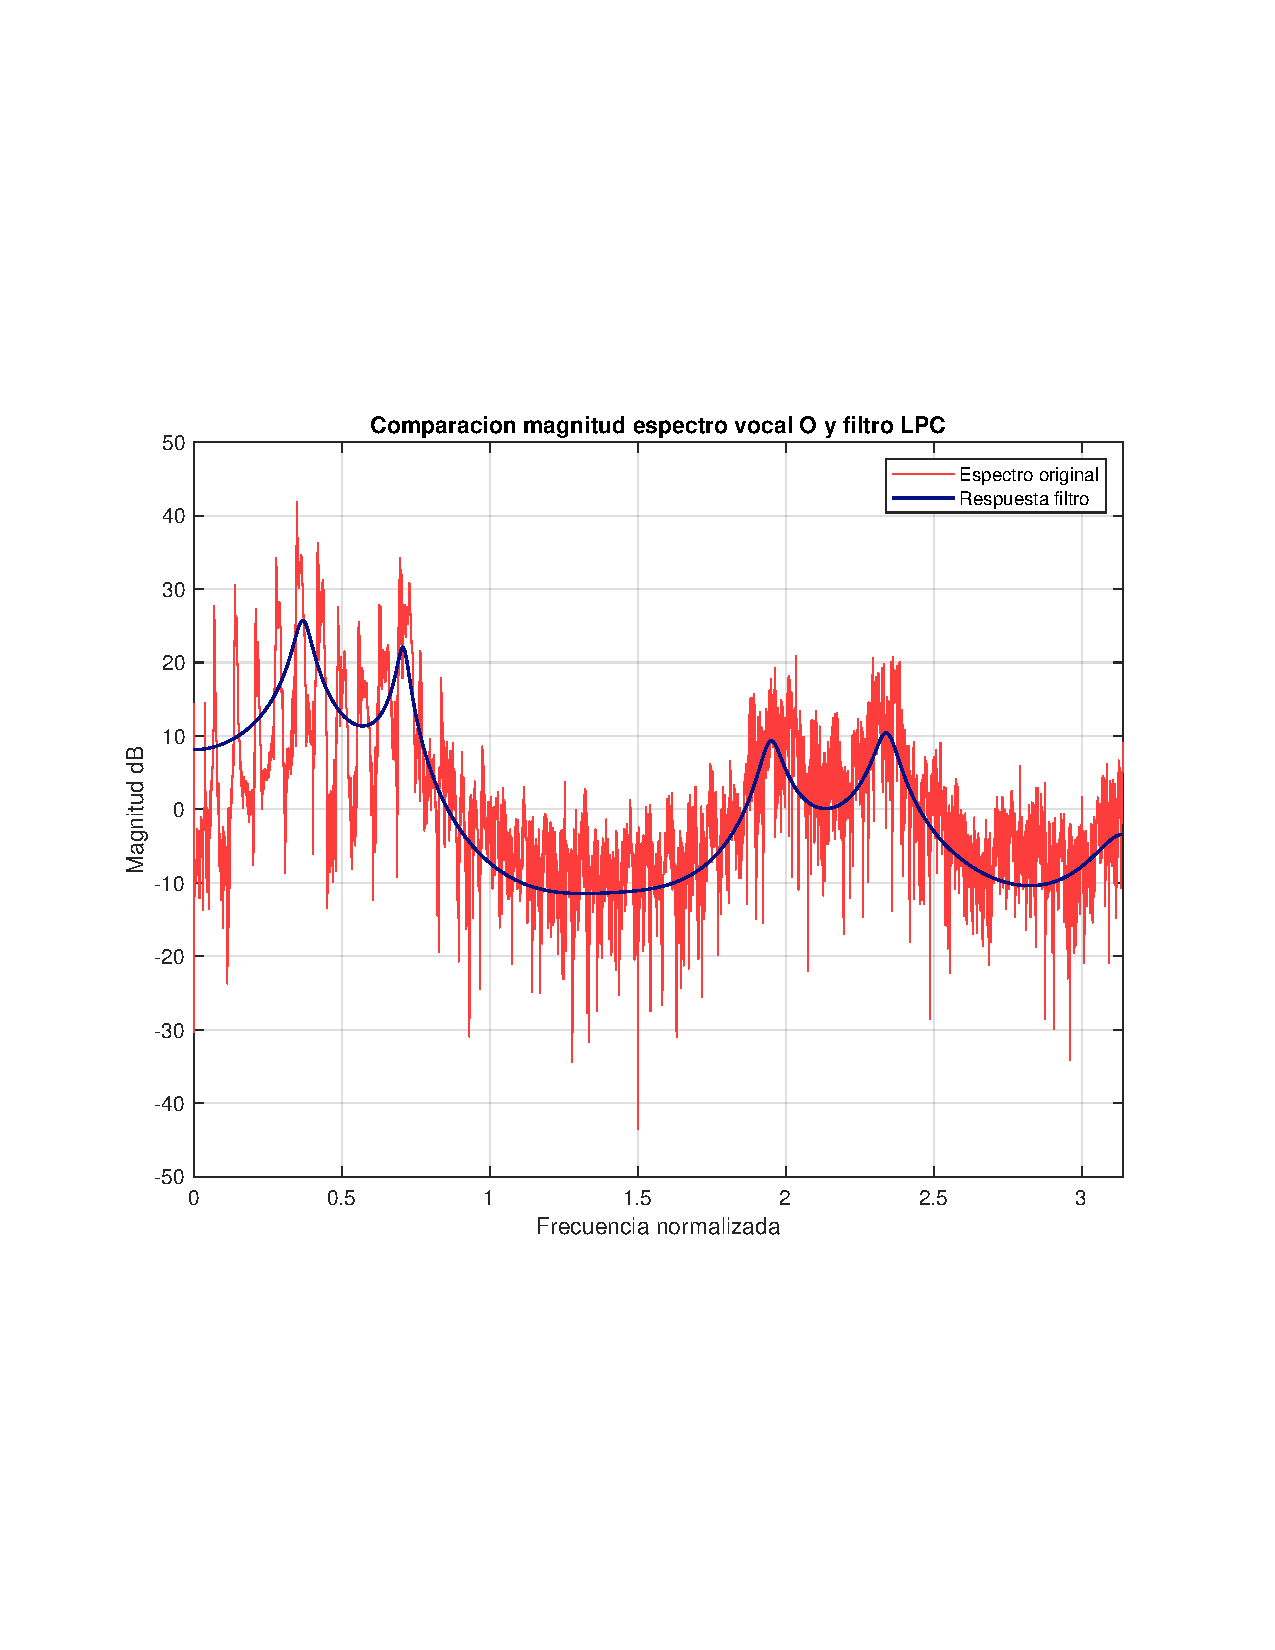
\includegraphics[width=0.6\textwidth,clip, trim = {1.9cm 6.8cm 2.3cm 7cm}]{../plots/O_lpc.pdf}
		\caption{Comparación espectro y filtro LPC: O}
		\label{fig:LPC_O}
	\end{figure}

	\begin{figure}[H]
		\center
		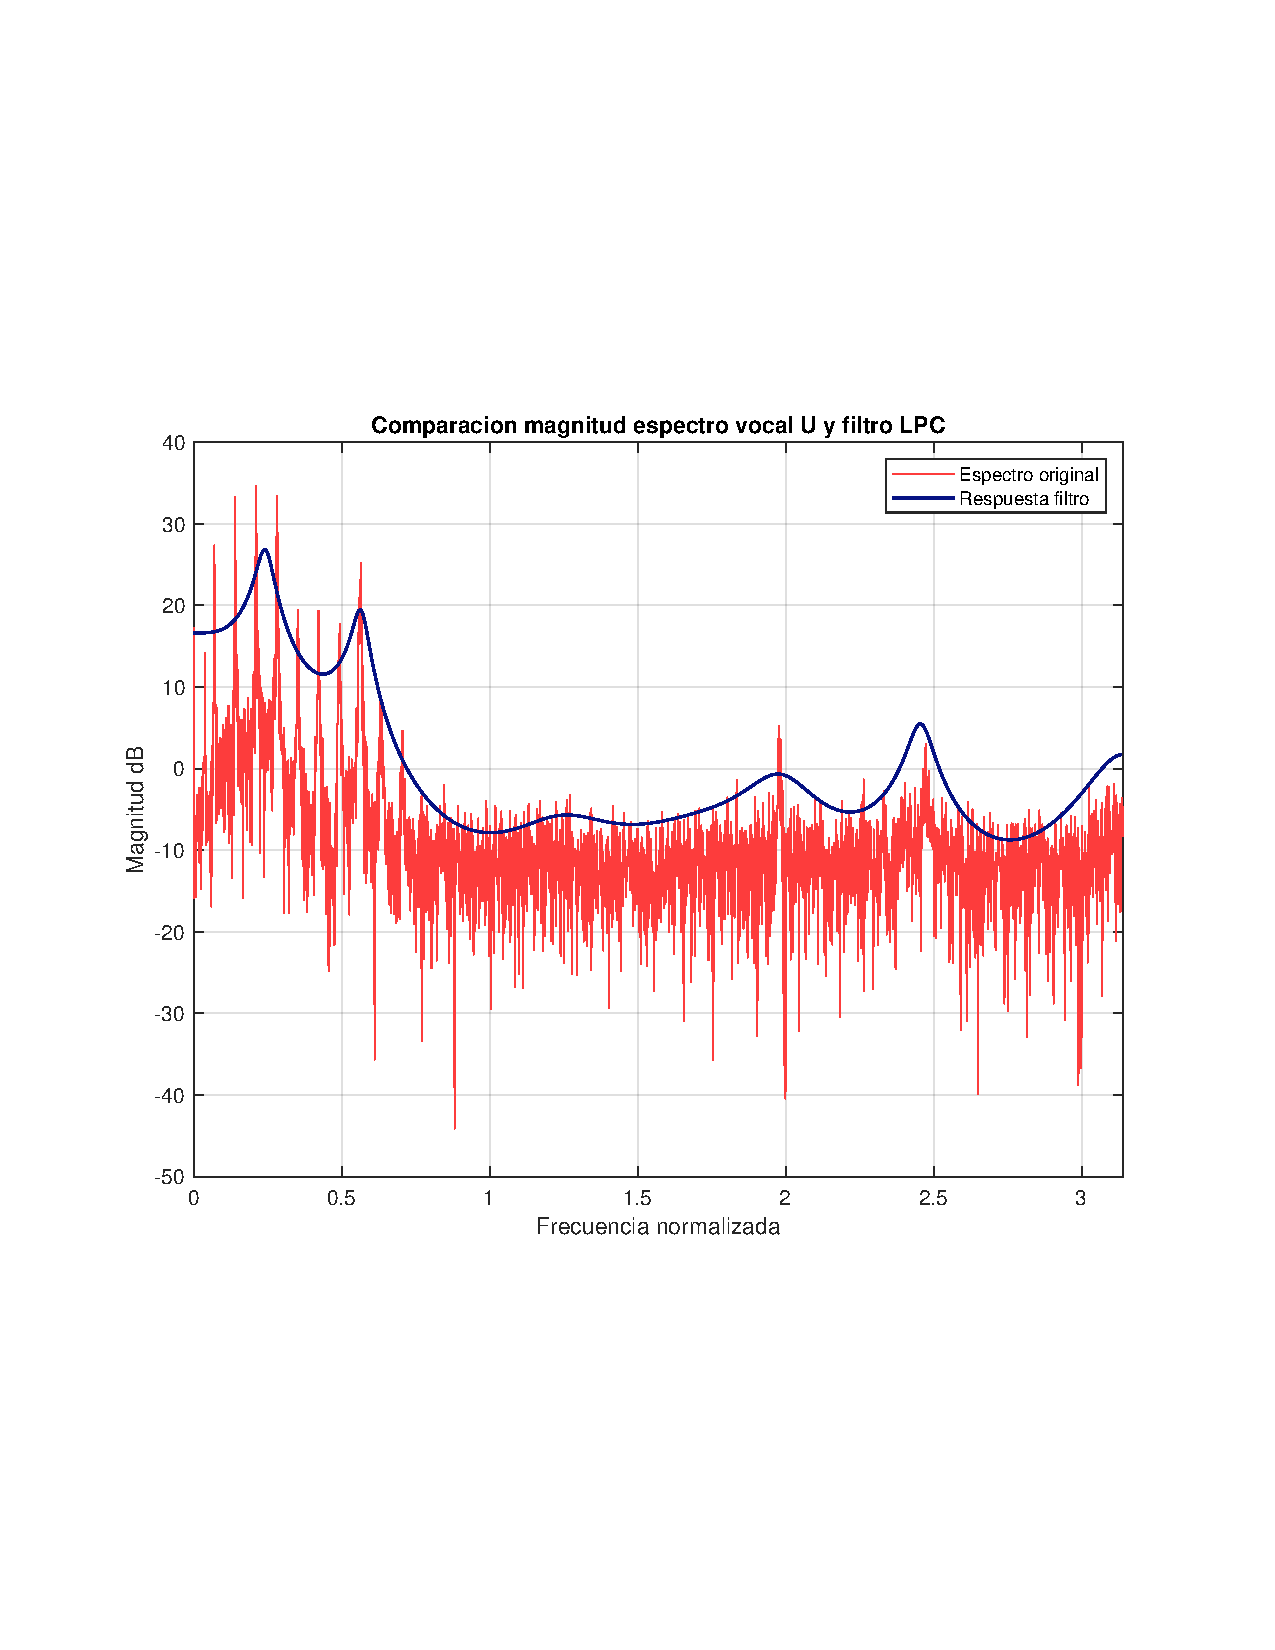
\includegraphics[width=0.6\textwidth,clip, trim = {1.9cm 6.8cm 2.3cm 7cm}]{../plots/U_lpc.pdf}
		\caption{Comparación espectro y filtro LPC: U}
		\label{fig:LPC_U}
	\end{figure}
	
	Se puede ver, que el resultado del filtro obtenido mediante LPC, permite tener una respuesta similar a la envolvente de la magnitud del espectro de la vocal. A partir de esto, se vuelve a obtener las formantes para cada vocal:
	\begin{table}[H]
		\center
		\begin{tabular}{|c|c|c|}
			\hline
			\textbf{Vocal}  & \textbf{F1 Hz} & \textbf{F2 Hz} \\
			\hline 
			A & 772 & 1273 \\
			\hline
			E & 420 & 2050 \\
			\hline
			I & 225 & 2444 \\
			\hline
			O & 468 & 898 \\
			\hline
			U & 304 & 718\\
			\hline
		\end{tabular}
		\caption{Tabla de frecuencia fundamental y formantes, para las distintas vocales, obtenidas mediante LPC}
		\label{tab:formantes-freq_lpc}
	\end{table}
	
	Comparando con lo obtenido en el punto anterior, tabla \ref{tab:formantes-freq}, se puede ver que los valores se mantuvieron aproximadamente constantes, graficando un nuevo triangulo vocálico:
	\begin{figure}[H]
		\center
		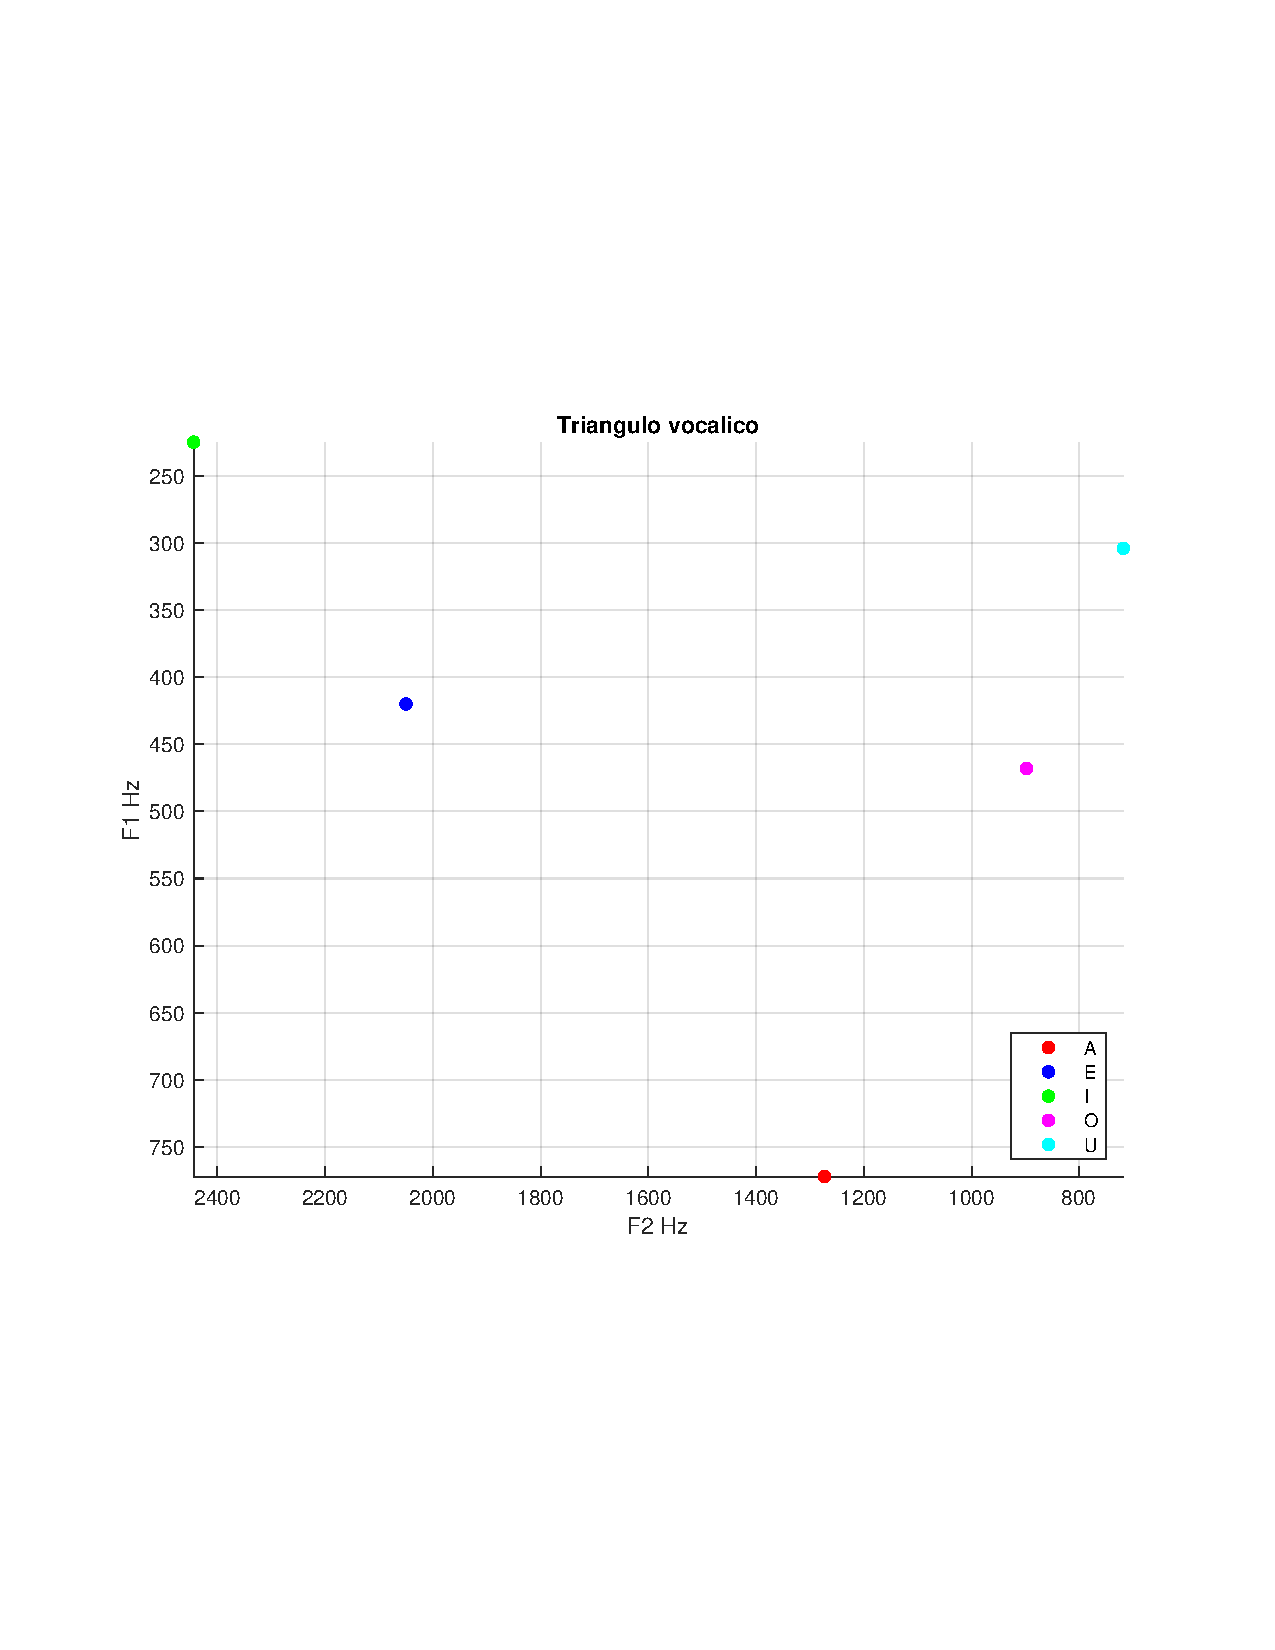
\includegraphics[width=0.6\textwidth,clip, trim = {1.9cm 6.8cm 2.3cm 7cm}]{../plots/vocalic_triang_2.pdf}
		\caption{Triángulo vocálico obtenido mediante LPC}
		\label{fig:vocal_triang_LPC}
	\end{figure}
	
	Realizando la comparación directa con el triangulo obtenido en figura \ref{fig:vocal_triang}:
	\begin{figure}[H]
		\center
		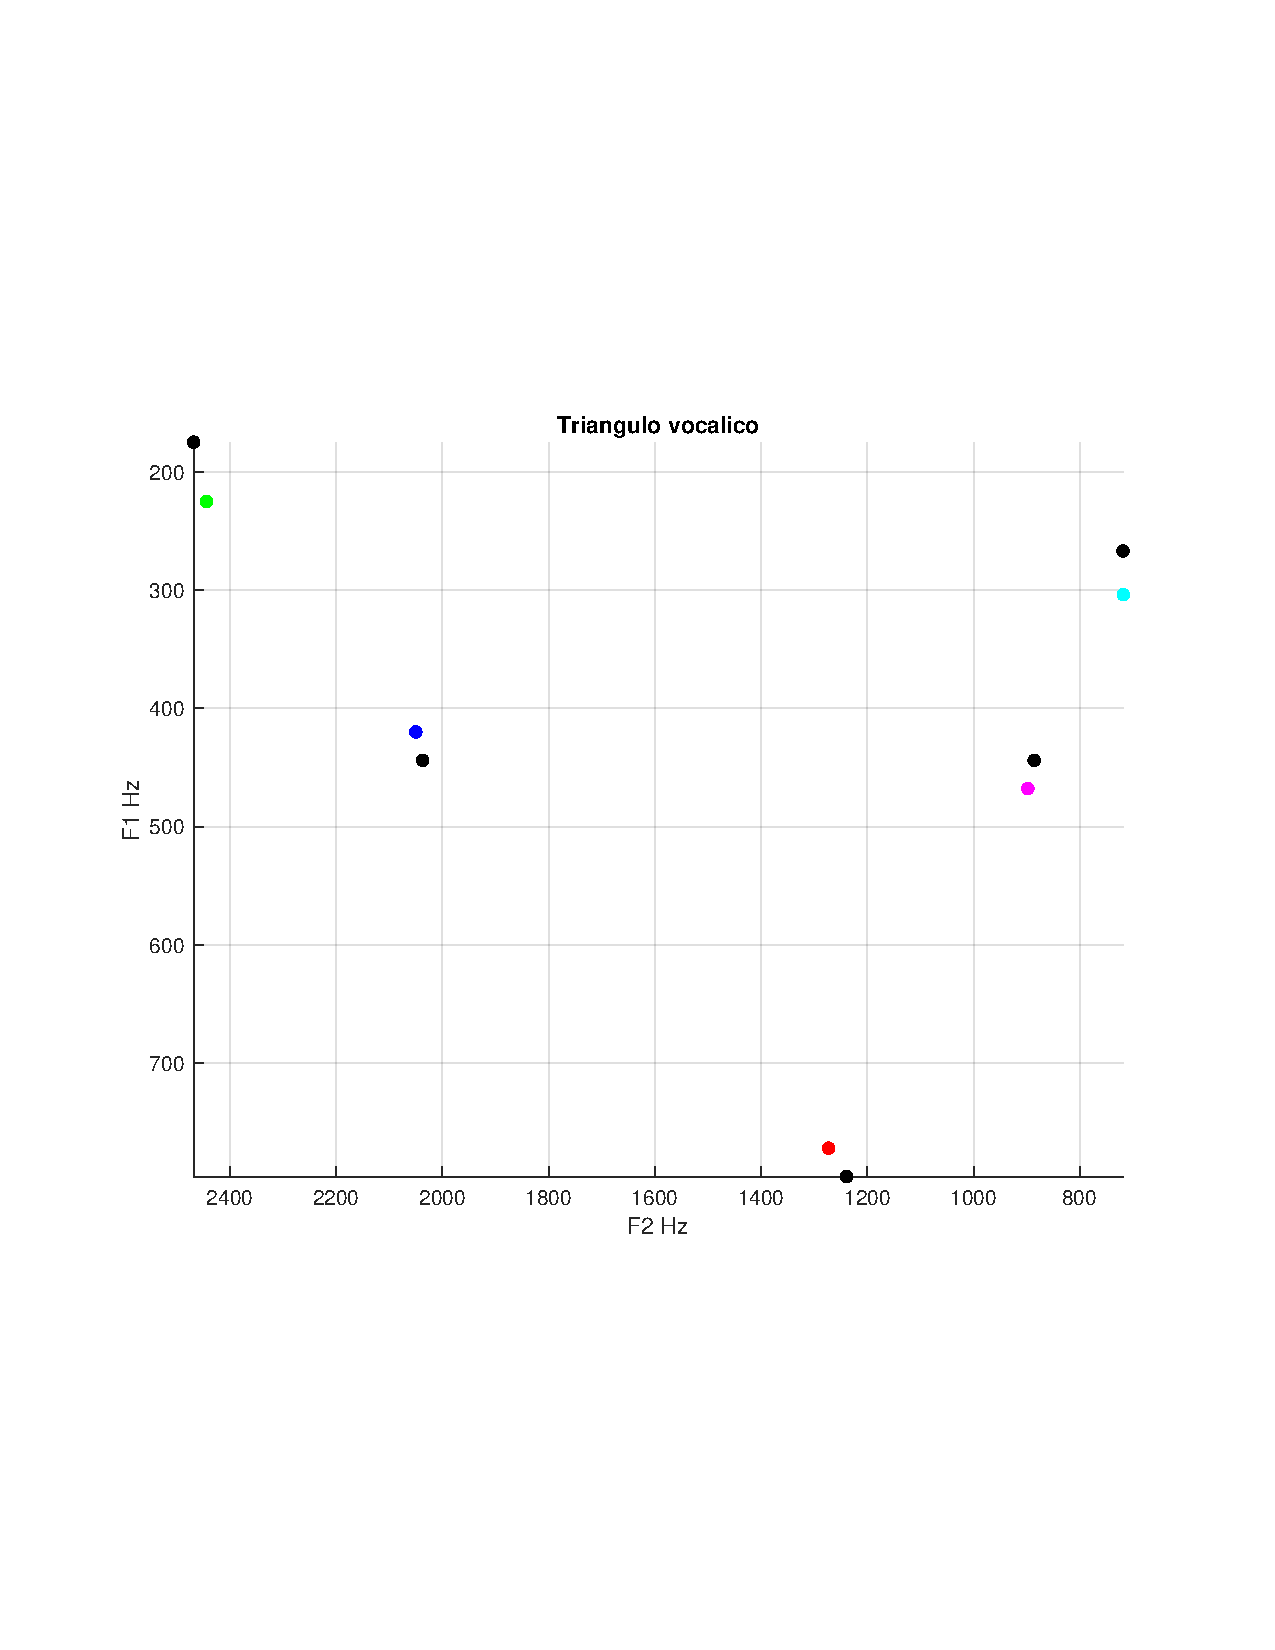
\includegraphics[width=0.6\textwidth,clip, trim = {1.9cm 6.8cm 2.3cm 7cm}]{../plots/vocalico_comp.pdf}
		\caption{Comparación triángulo vocálico obtenido mediante LPC (en colores) y comparación triangulo obtenido desde el espectro (negro).}
		\label{fig:vocal_triang_LPC_comparative}
	\end{figure}
	
	A partir de esto, se puede ver que el movimiento de las formantes, para las vocales es mínimo y siguen estando bastante cerca de las formantes obtenidas del espectro, por lo que se puede concluir que el filtro representa de manera fiel la envolvente asociada al espectro de cada vocal.
	
\section{Espectrograma}
	\subsection{Construcción de espectrogramas}
	Utilizando la función implementada \texttt{DFTwin}, se procede a calcular el espectro de la vocal \textit{a}, considerando que interesa únicamente, seis períodos de oscilación de la frecuencia fundamental:
	\begin{equation*}
		6 \cdot \frac{1}{f0} = \frac{6}{87} \approx 0.0689~\text{s}
	\end{equation*}
	
	Llevando esto a muestras:
	\begin{equation*}
		S = ceil \left( \frac{6 \cdot fs}{f0} \right) = 552~\text{muestras}
	\end{equation*}
	
	Se sabe que las señales de vocales en general comienzan en la muestra $m = 5000$. Para la resolución espectral, se escoge el mismo largo de la señal, en este caso $N = 552$. Por lo que la función utilizada queda definida como \texttt{DFTwin(a, 552,5000, 552)}. Graficando la magnitud del espectro:
	
	\begin{figure}[H]
		\center
		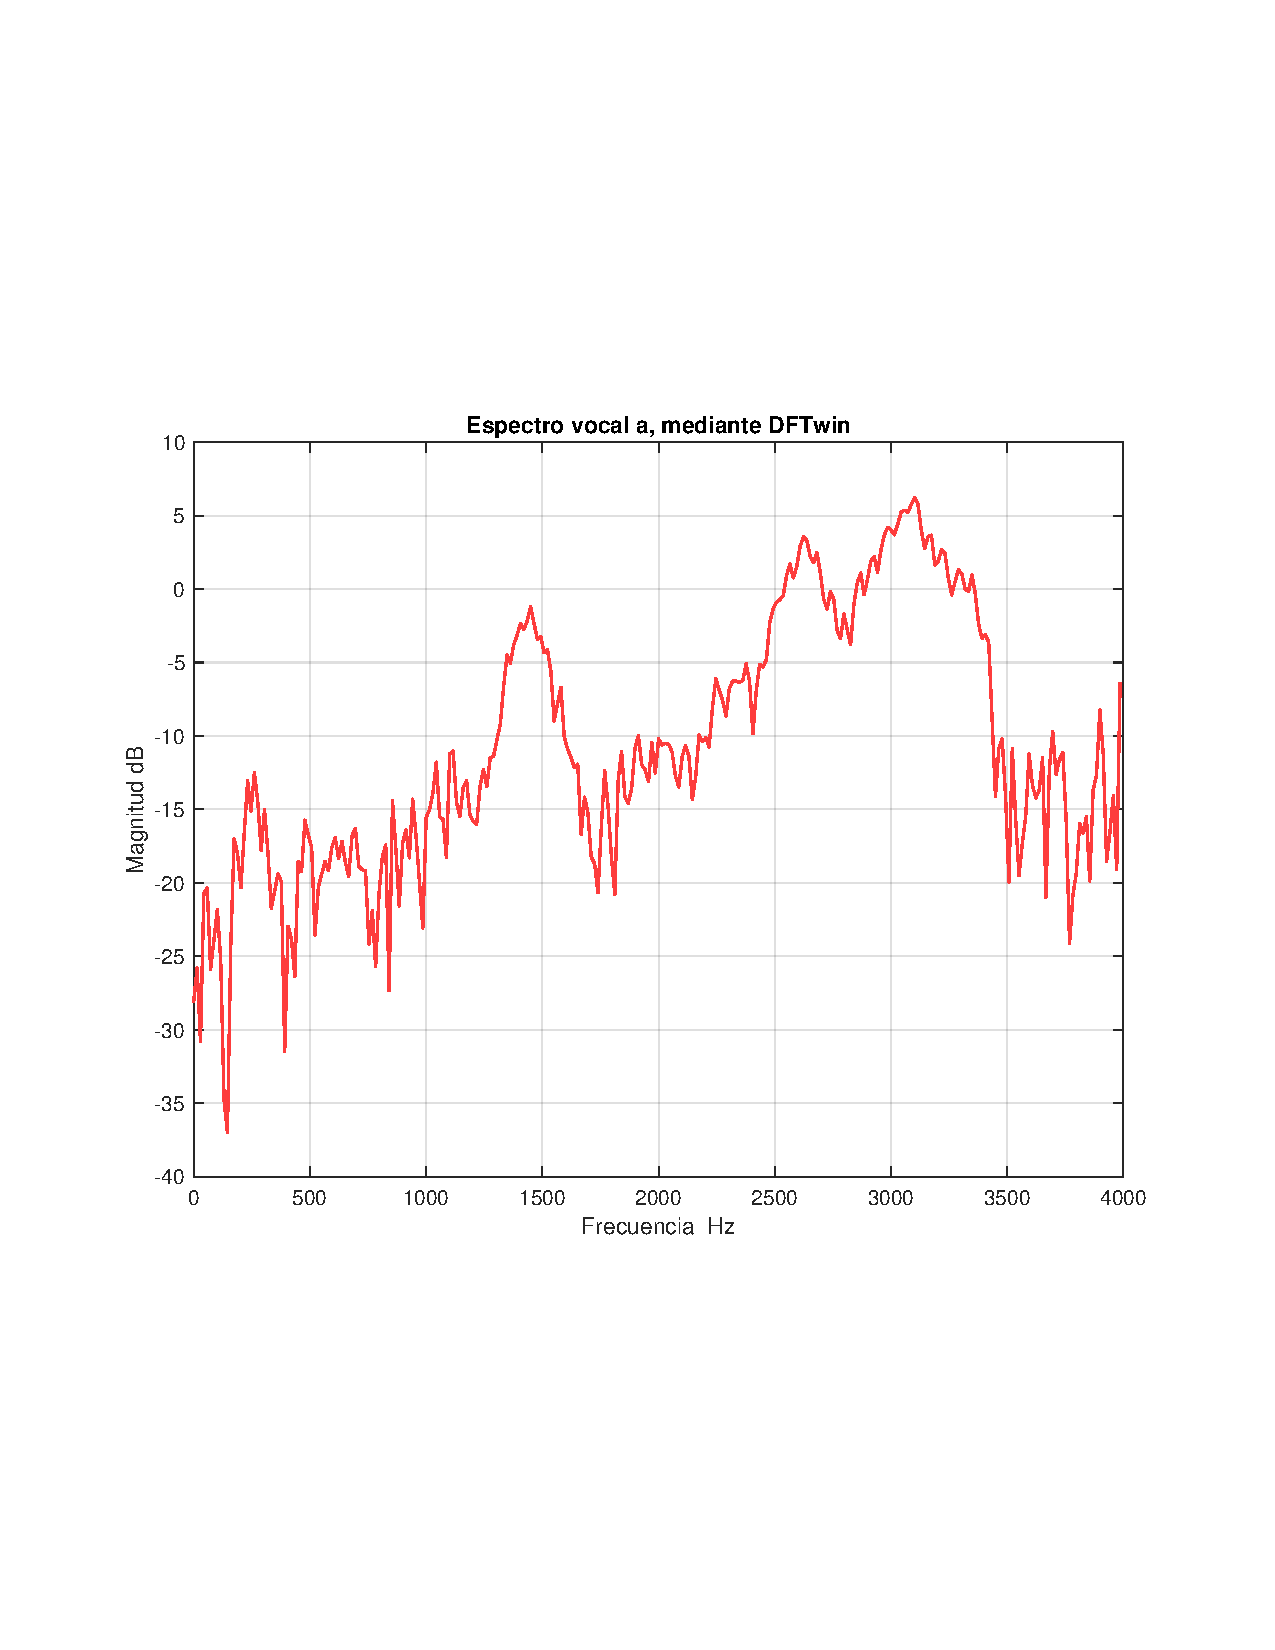
\includegraphics[width=0.6\textwidth,clip, trim = {1.9cm 6.8cm 2.3cm 7cm}]{../plots/a_dftwin.pdf}
		\caption{Espectro de la vocal a, para seis períodos de oscilación}
		\label{fig:fft_6_f0}
	\end{figure}


%\newpage
\section{Maybe later}
		 Aplicando la propiedad de la suma en el coseno, se puede descomponer esta expresión:
		 \begin{equation*}
		 	x[n] = 2 \left ( cos(\frac{\pi}{6}n) \cdot cos(\frac{pi}{4}) - sin(\frac{\pi n}{6} \cdot sin(\frac{\pi}{4} \right)
		 \end{equation*}
		 
		 Con $cos(\pi/4) = \sqrt(2)/2$:
		 \begin{equation*}
		 	x[n] = \sqrt{2} \left( cos(\frac{\pi n }{6} - sin(\frac{\pi n}{6}) \right)
		 \end{equation*}		  
		
		Note 
		

\end{document}
